\chapter{Prezentacja warstwy użytkowej projektu}

\section{Panel logowania oraz rejestracji}

Panel logowania umożliwia użytkownikowi 
uwierzytelnienie się w systemie. Formularz zawiera dwa pola: adres e-mail oraz hasło. Po 
kliknięciu przycisku Zaloguj się aplikacja weryfikuje poprawność wprowadzonych danych. Po poprawnym 
zalogowaniu użytkownik zostaje przekierowany do panelu użytkownika lub panelu administratora, w z
ależności od przypisanej roli. Użytkownik nieposiadający konta może przejść do formularza rejestracji klikając przycisk Zarejestruj się.

\begin{figure}[H]
\centering
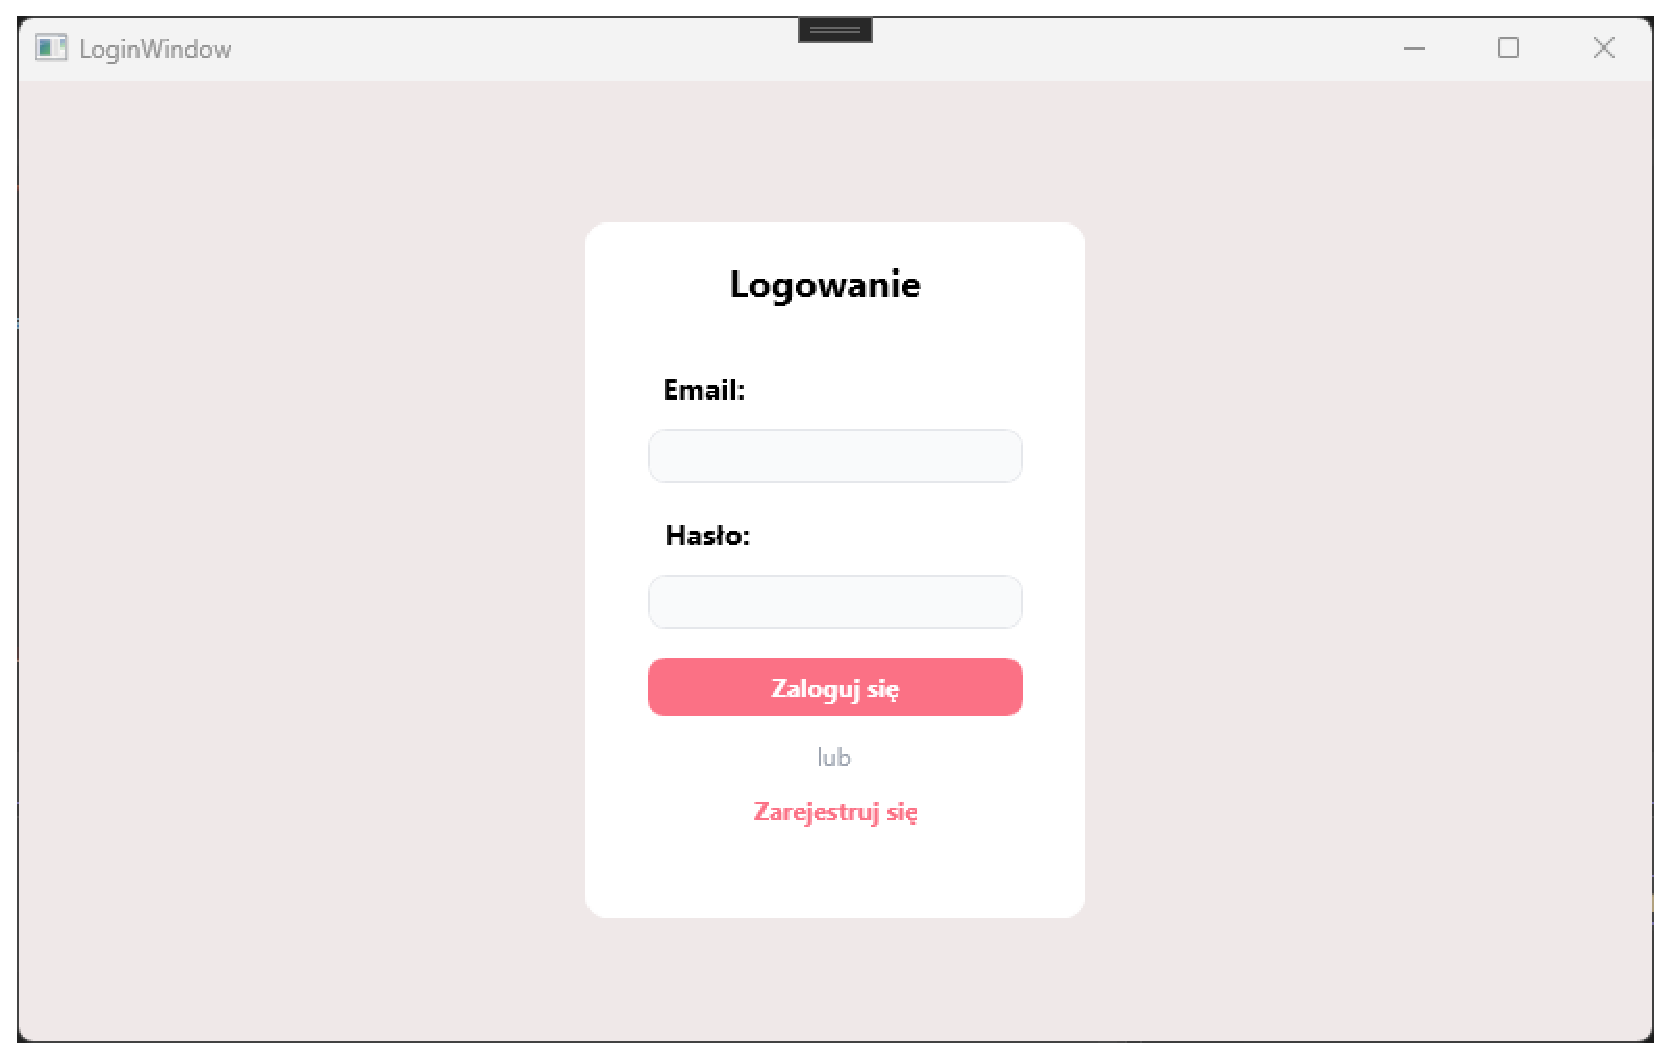
\includegraphics[width=0.8\linewidth]{figures/Logowanie/fig_005.eps}
\caption{Widok panelu logowania.\label{fig5}}
\end{figure}

W przypadku gdy użytkownik nie wypełni pól formularza lub poda błędne dane logowania, wyświetlany jest 
komunikat błędu informujący o nieprawidłowym adresie e-mail lub haśle.

\begin{figure}[H]
\centering
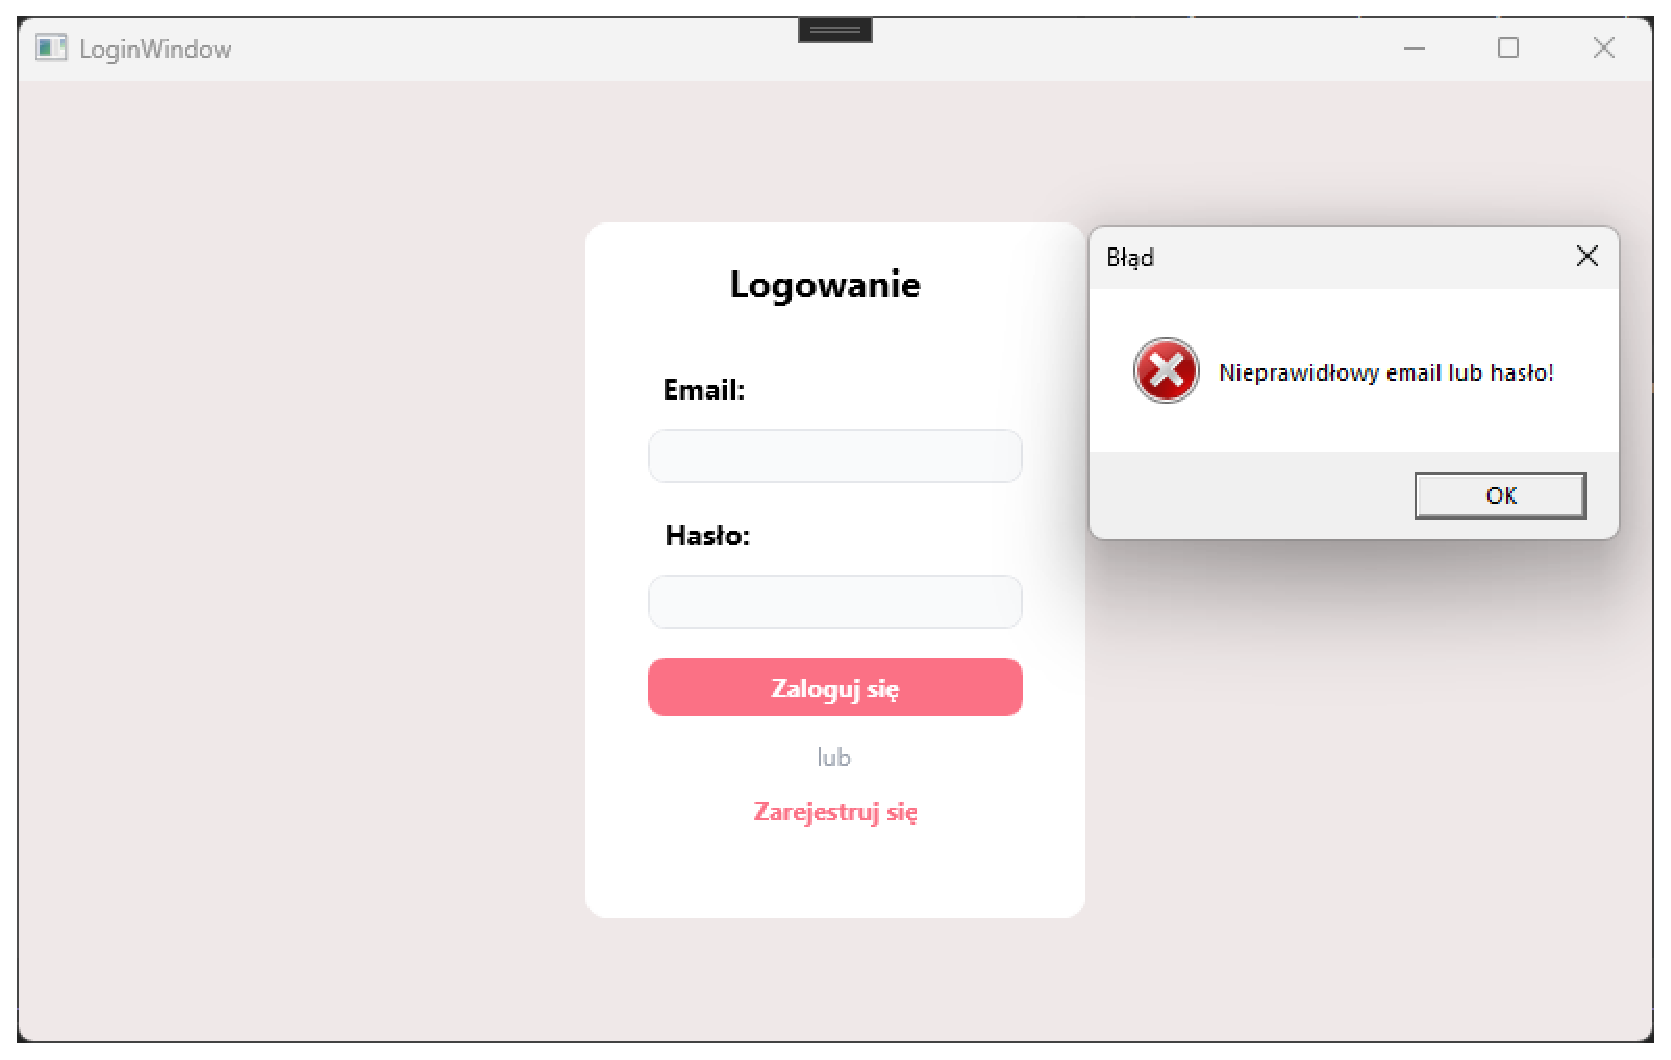
\includegraphics[width=0.8\linewidth]{figures/Logowanie/fig_006.eps}
\caption{Komunikat błędu przy nieprawidłowych danych logowania.\label{fig6}}
\end{figure}

\textbf{Panel rejestracji}

Panel rejestracji umożliwia nowemu użytkownikowi założenie konta w systemie. Formularz zawiera pola: imię, 
nazwisko, adres e-mail, numer telefonu, adres (pole opcjonalne), hasło oraz potwierdzenie hasła. 
Po wypełnieniu formularza i kliknięciu przycisku Zarejestruj się aplikacja przeprowadza 
wieloetapową walidację danych. Użytkownik posiadający już konto może powrócić do ekranu logowania klikając przycisk Powróć do logowania.

\begin{figure}[H]
\centering
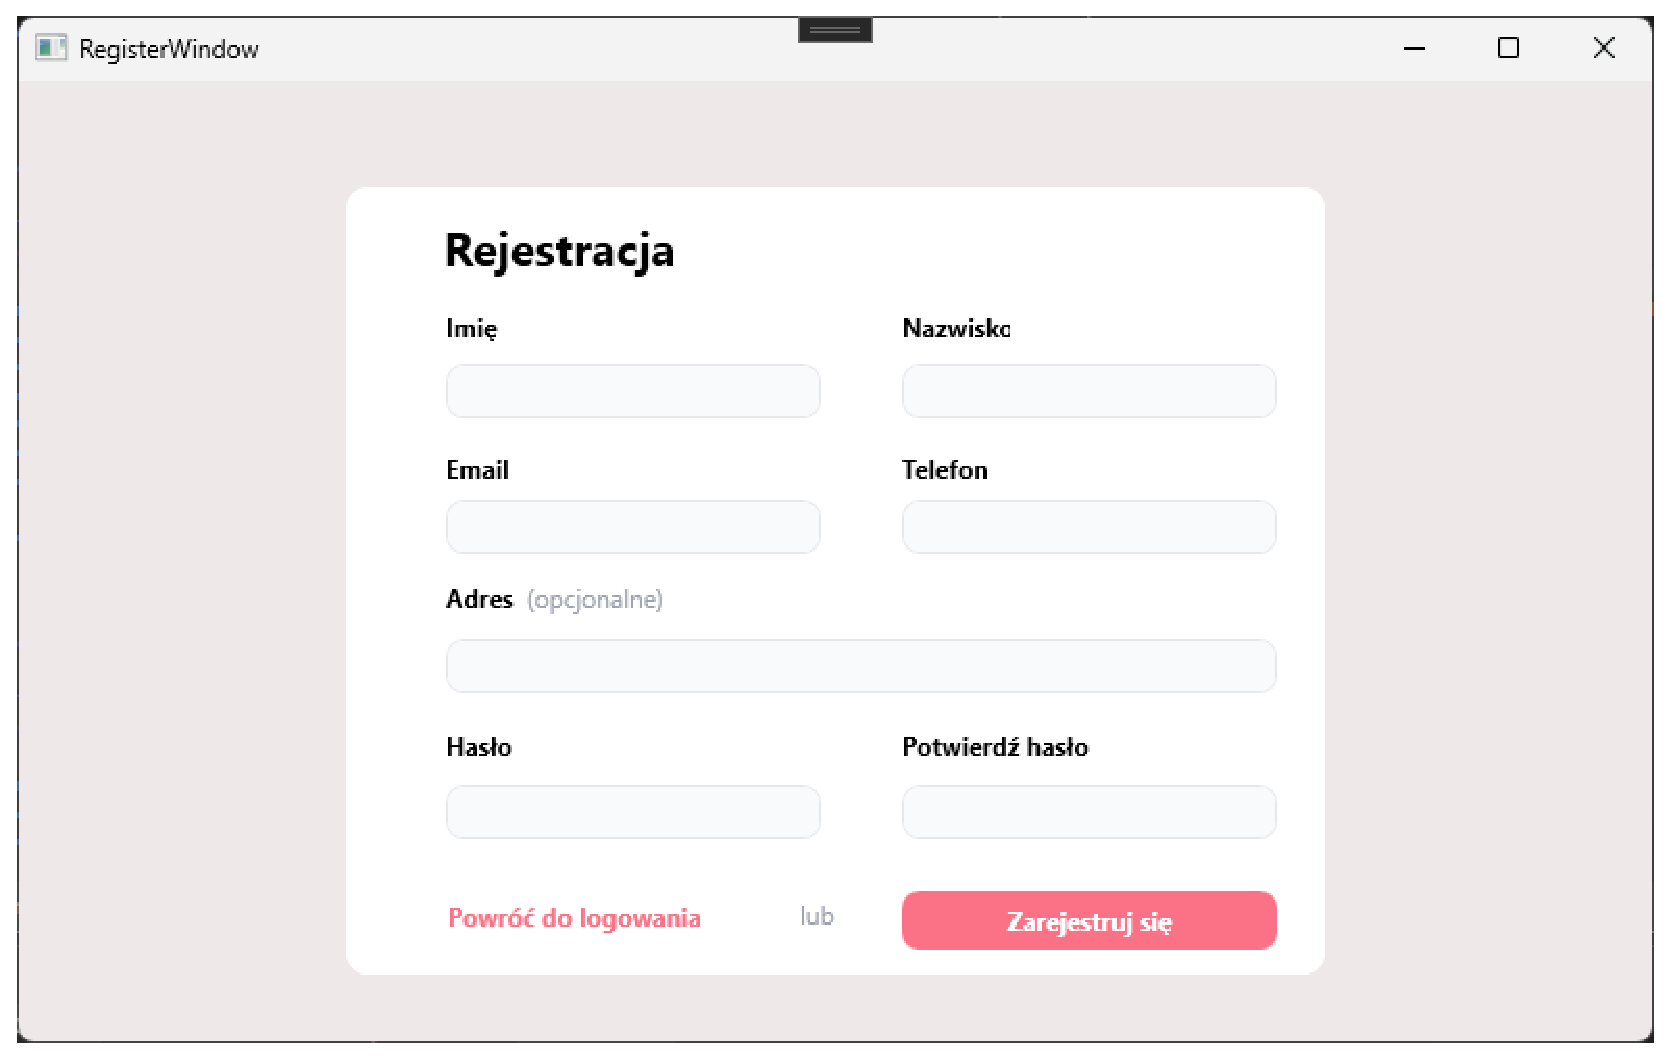
\includegraphics[width=0.8\linewidth]{figures/Rejestracja/fig_007.eps}
\caption{Widok panelu rejestracji.\label{fig7}}
\end{figure}

W przypadku gdy użytkownik nie wypełni wszystkich wymaganych pól formularza, wyświetlany jest komunikat błędu informujący o konieczności uzupełnienia danych.

\begin{figure}[H]
\centering
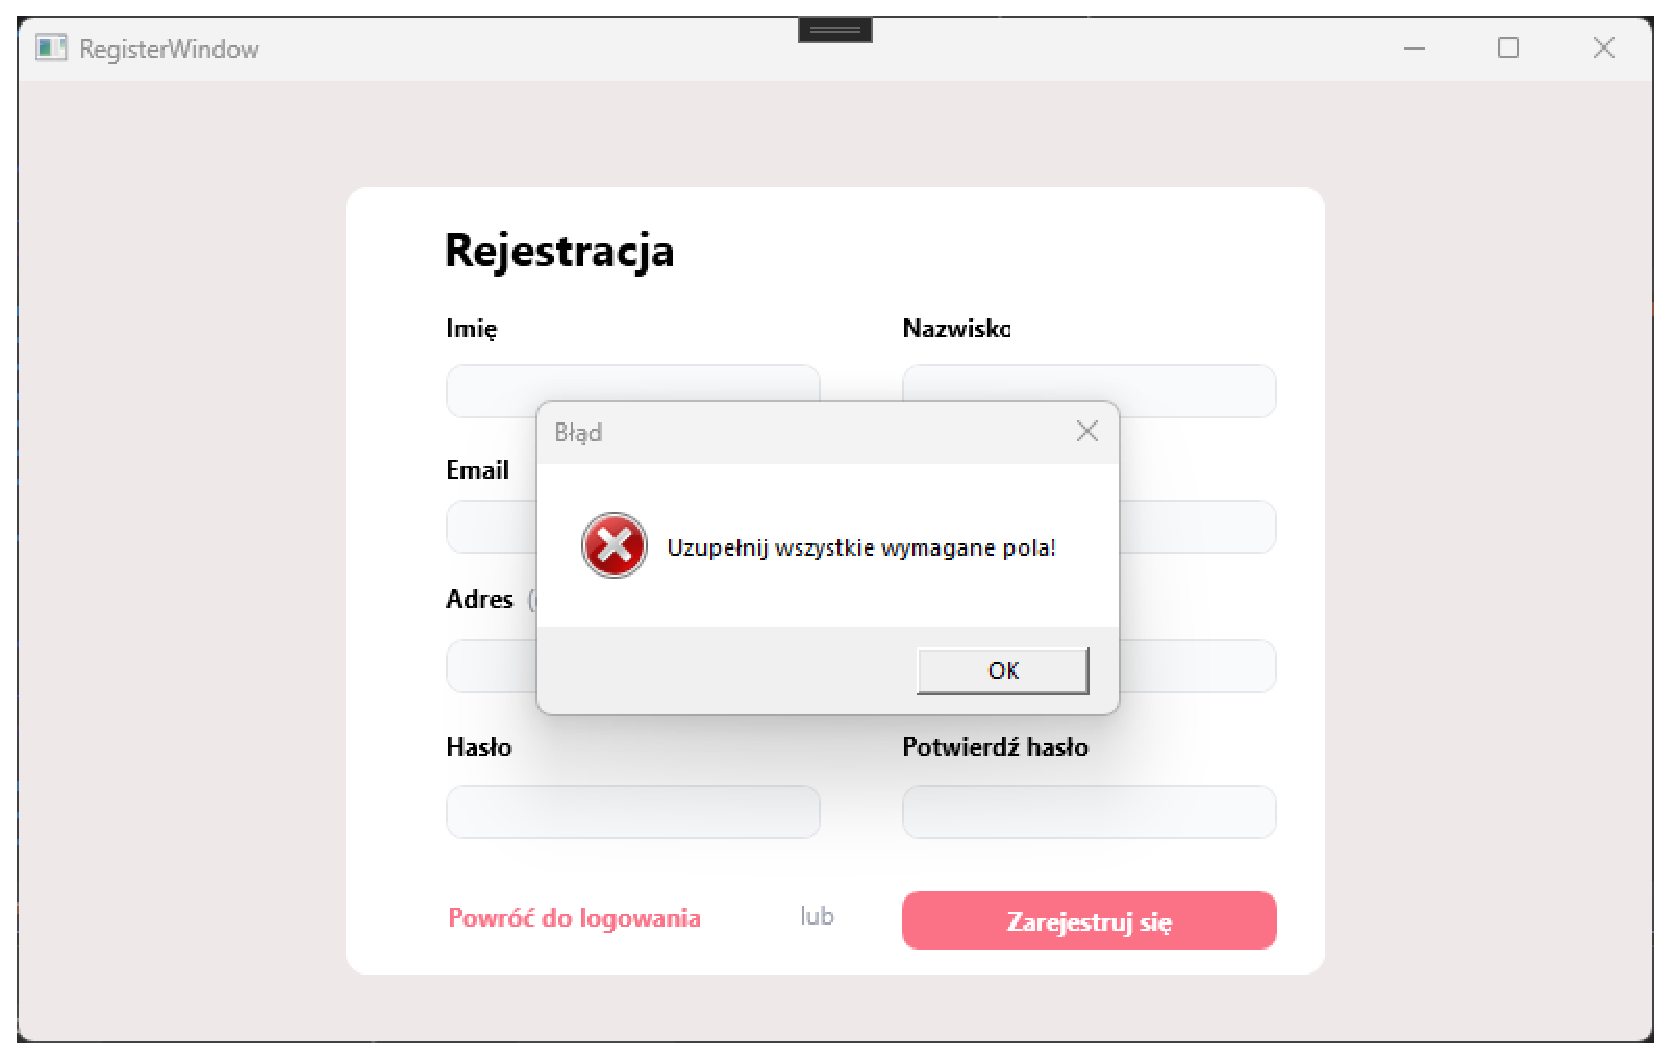
\includegraphics[width=0.8\linewidth]{figures/Rejestracja/fig_008.eps}
\caption{Komunikat błędu przy niewypełnionych polach formularza.\label{fig8}}
\end{figure}

Aplikacja weryfikuje również poprawność formatu numeru telefonu tzn. numer musi składać się z dokładnie 9 cyfr oraz nie zawierać innych znaków. 
W przypadku podania numeru w nieprawidłowym formacie wyświetlany jest odpowiedni komunikat błędu.

\begin{figure}[H]
\centering
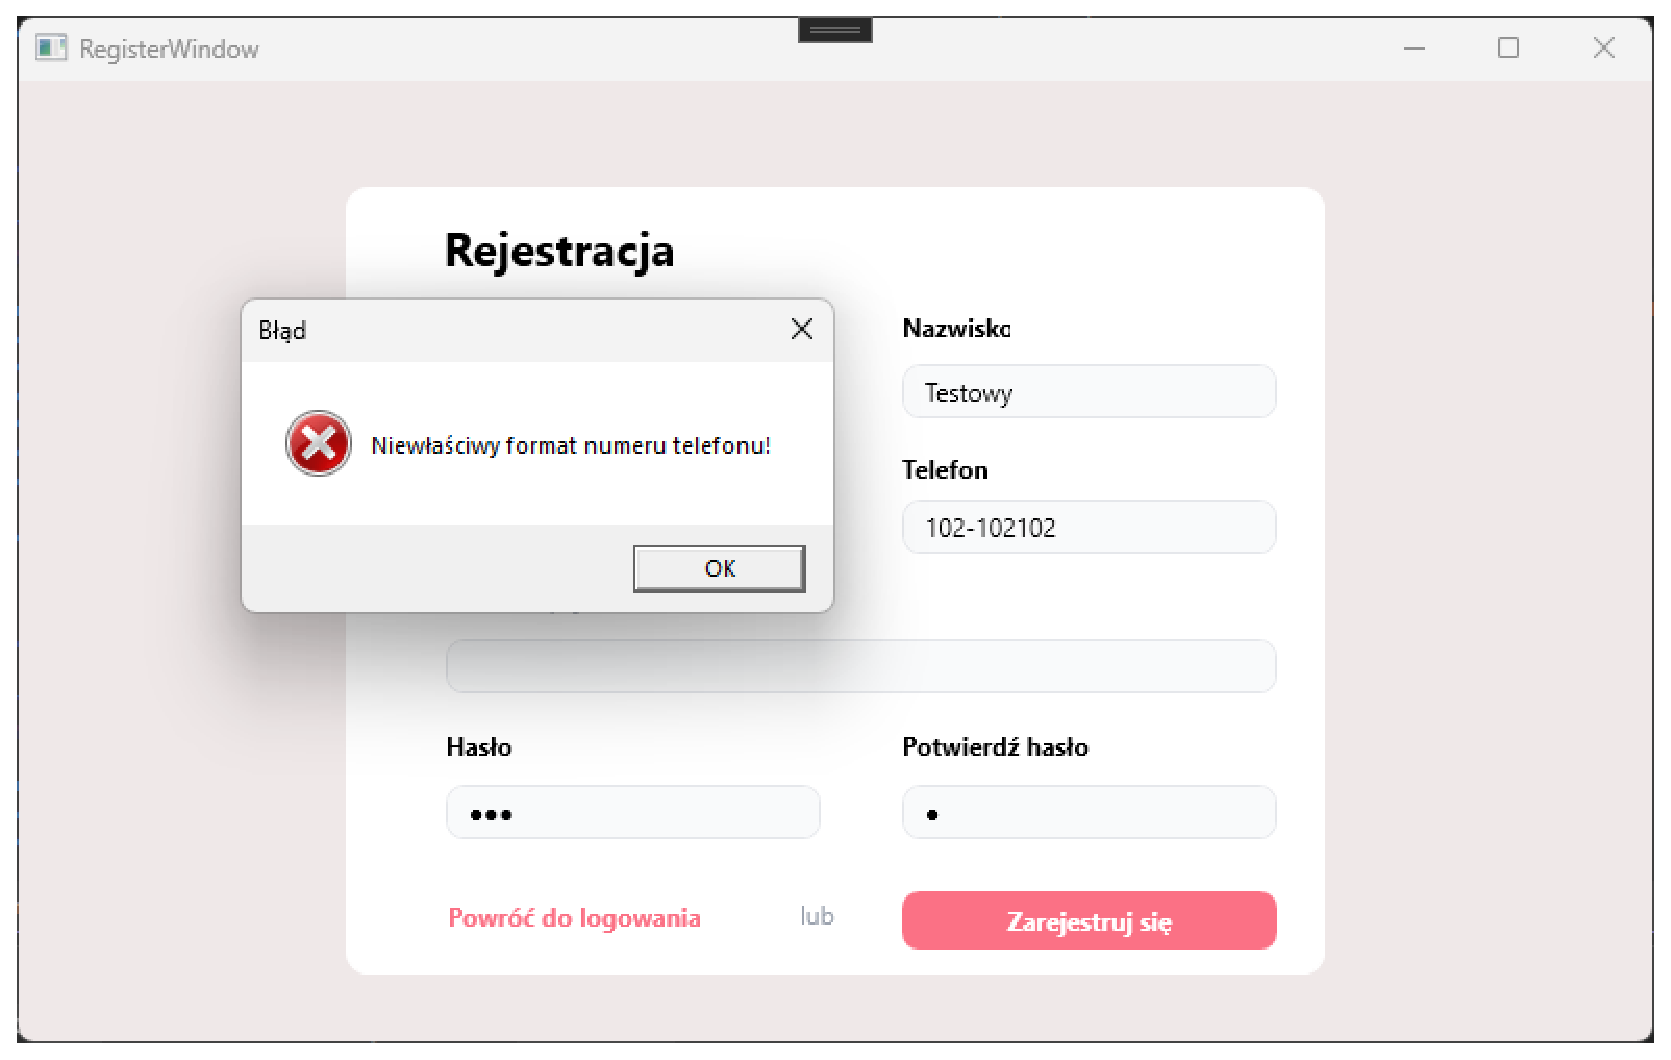
\includegraphics[width=0.8\linewidth]{figures/Rejestracja/fig_009.eps}
\caption{Komunikat błędu przy nieprawidłowym formacie numeru telefonu.\label{fig9}}
\end{figure}

Kolejnym etapem walidacji jest sprawdzenie, czy podane hasło i jego potwierdzenie są identyczne. W przypadku niezgodności haseł wyświetlany jest komunikat błędu.

\begin{figure}[H]
\centering
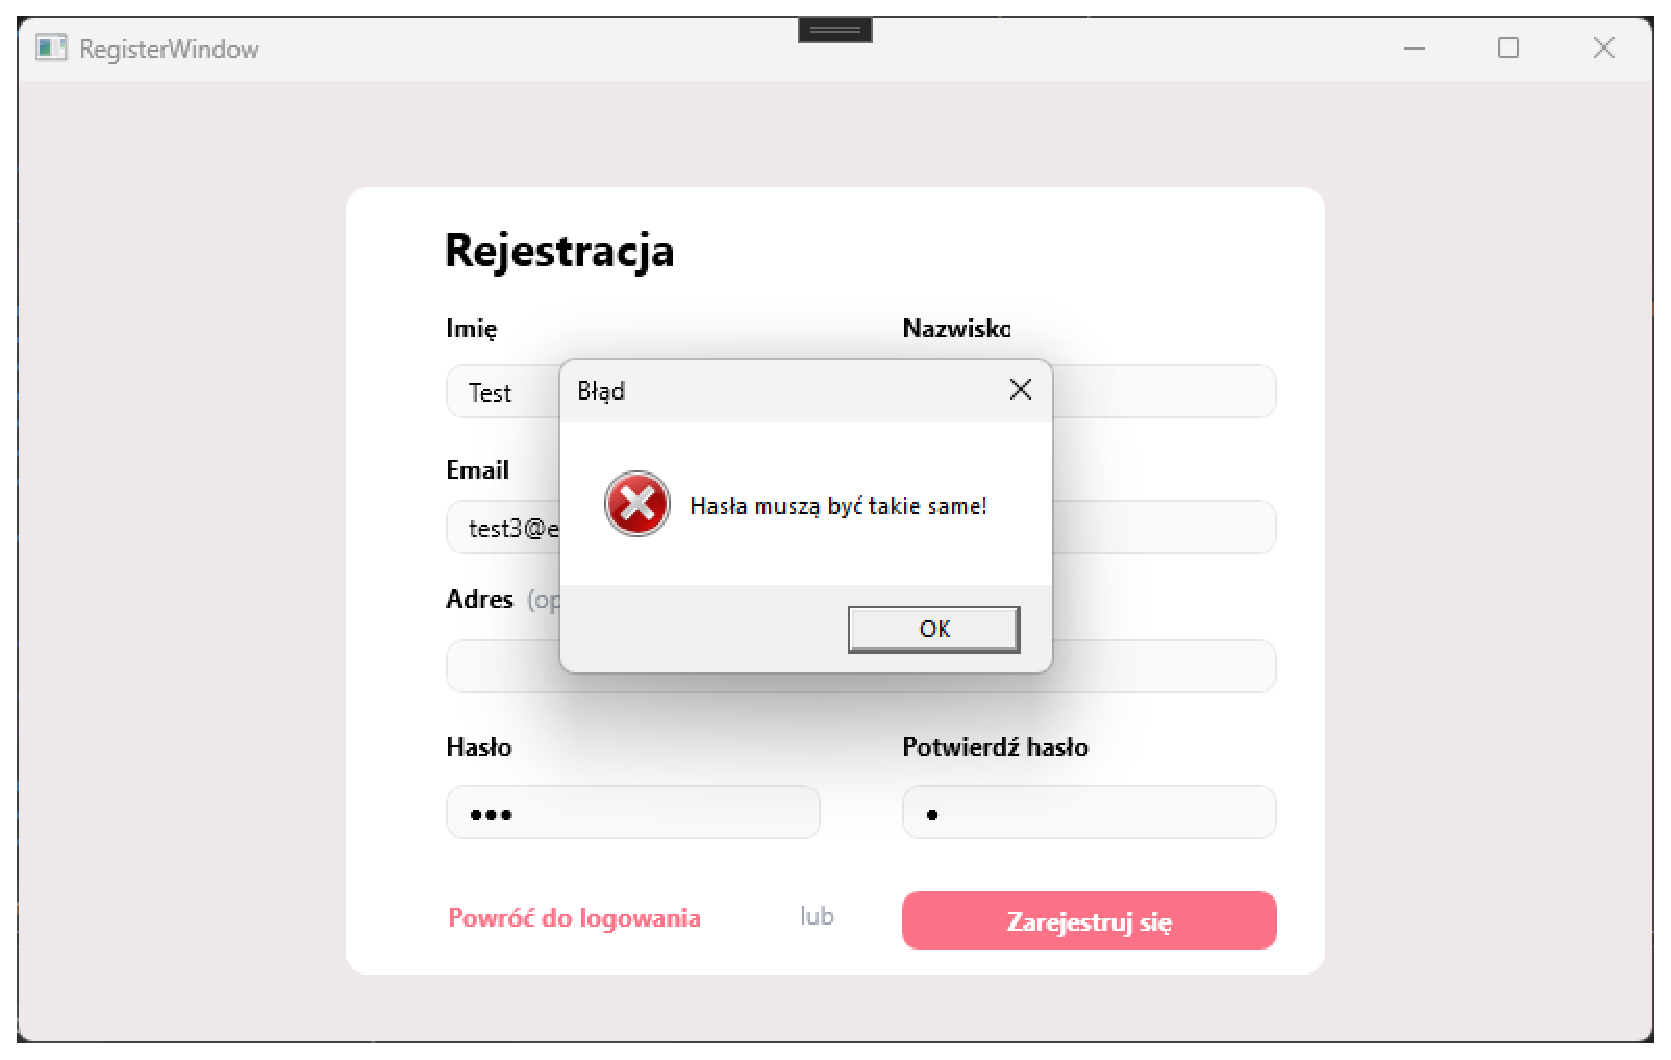
\includegraphics[width=0.8\linewidth]{figures/Rejestracja/fig_010.eps}
\caption{Komunikat błędu przy niezgodności haseł.\label{fig10}}
\end{figure}

Ostatnim etapem walidacji jest sprawdzenie długości hasła - musi ono zawierać co najmniej 6 znaków. W przypadku 
podania zbyt krótkiego hasła wyświetlany jest odpowiedni komunikat błędu.

\begin{figure}[H]
\centering
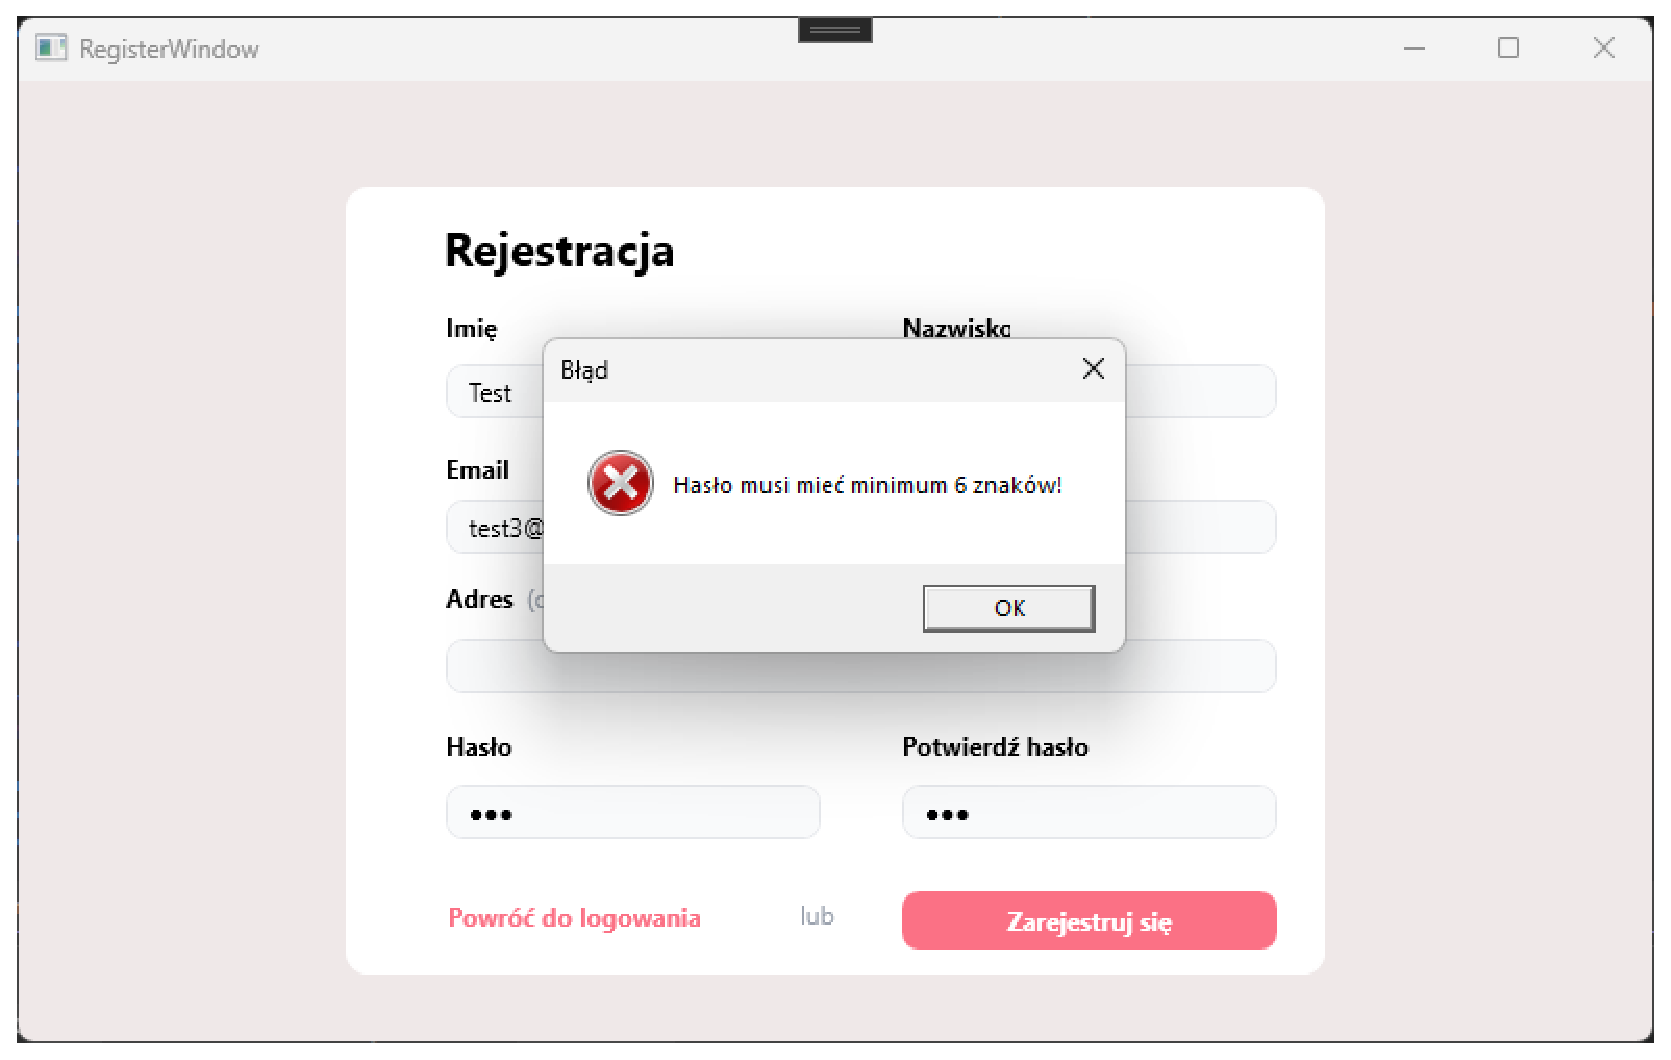
\includegraphics[width=0.8\linewidth]{figures/Rejestracja/fig_011.eps}
\caption{Komunikat błędu przy haśle krótszym niż 6 znaków.\label{fig11}}
\end{figure}

\section{Panel użytkownika}

\textbf{Zakładka "Moje konto"}

Zakładka "Moje konto" umożliwia zalogowanemu użytkownikowi przeglądanie i edycję swoich danych osobowych oraz 
zmianę hasła. W górnej części ekranu widoczny jest pasek nawigacyjny z nazwą kliniki, imieniem zalogowanego użytkownika, aktualnym 
saldem konta oraz przyciskiem wylogowania. Sekcja Twoje dane wyświetla imię, nazwisko, adres e-mail, numer telefonu 
oraz adres użytkownika wczytane automatycznie po zalogowaniu. Przycisk Zmień dane umożliwia zapisanie wprowadzonych zmian.

\begin{figure}[H]
\centering
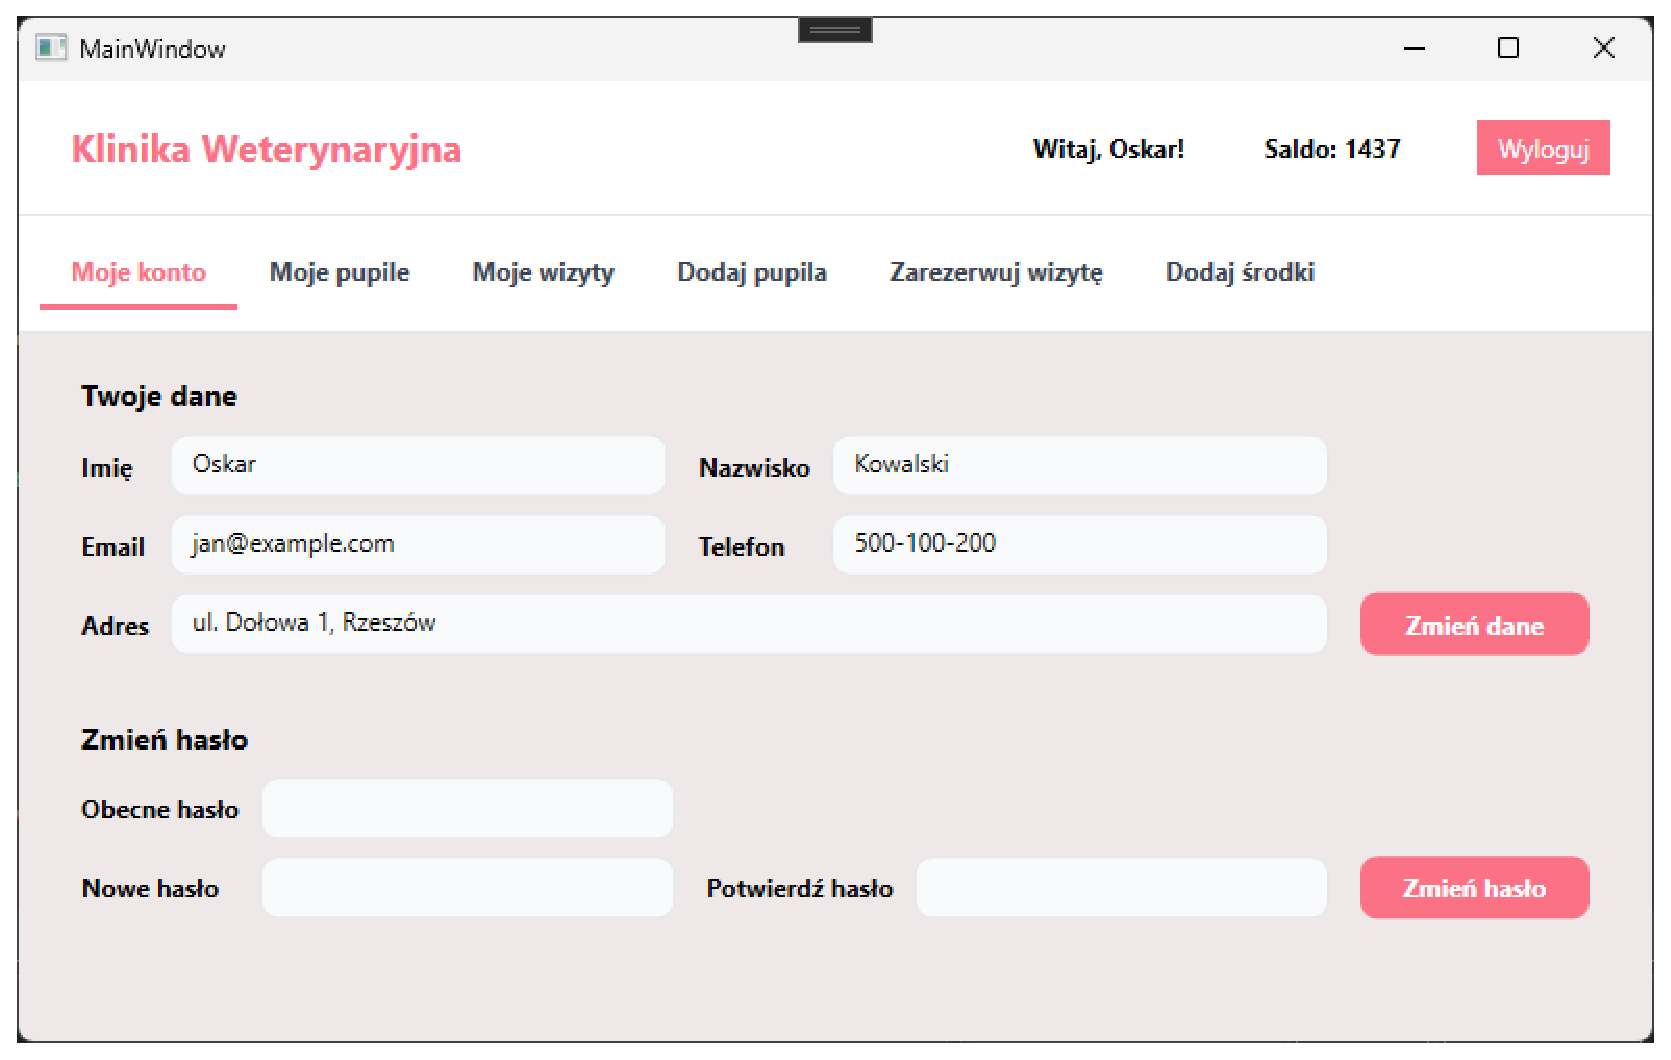
\includegraphics[width=0.9\linewidth]{figures/Uzytkownik/fig_012.eps}
\caption{Widok zakładki Moje konto.\label{fig12}}
\end{figure}

W przypadku kliknięcia przycisku Zmień dane bez wprowadzenia żadnych modyfikacji, aplikacja wyświetla 
komunikat informujący o konieczności wprowadzenia danych do zmiany.

\begin{figure}[H]
\centering
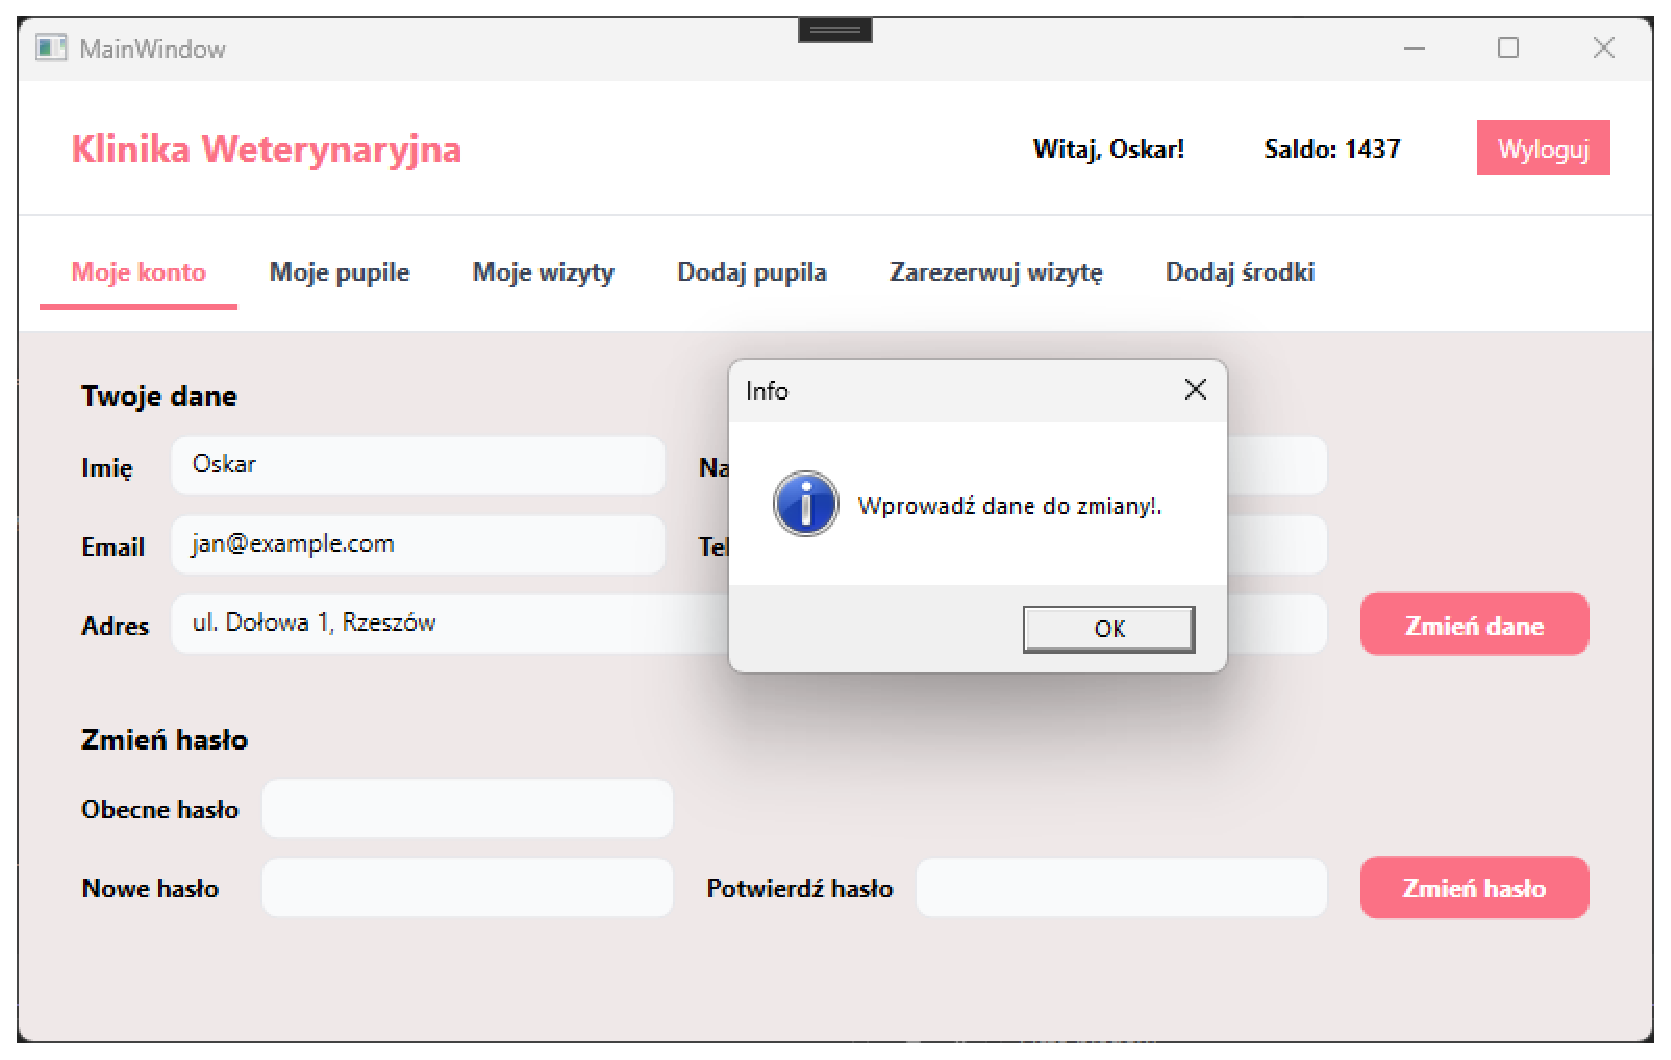
\includegraphics[width=0.9\linewidth]{figures/Uzytkownik/fig_013.eps}
\caption{Komunikat informacyjny przy braku zmian w danych.\label{fig13}}
\end{figure}

Sekcja Zmień hasło zawiera trzy pola: obecne hasło, nowe hasło oraz potwierdzenie nowego hasła. W przypadku gdy użytkownik nie wypełni wszystkich pól 
i kliknie przycisk Zmień hasło, wyświetlany jest komunikat błędu.

\begin{figure}[H]
\centering
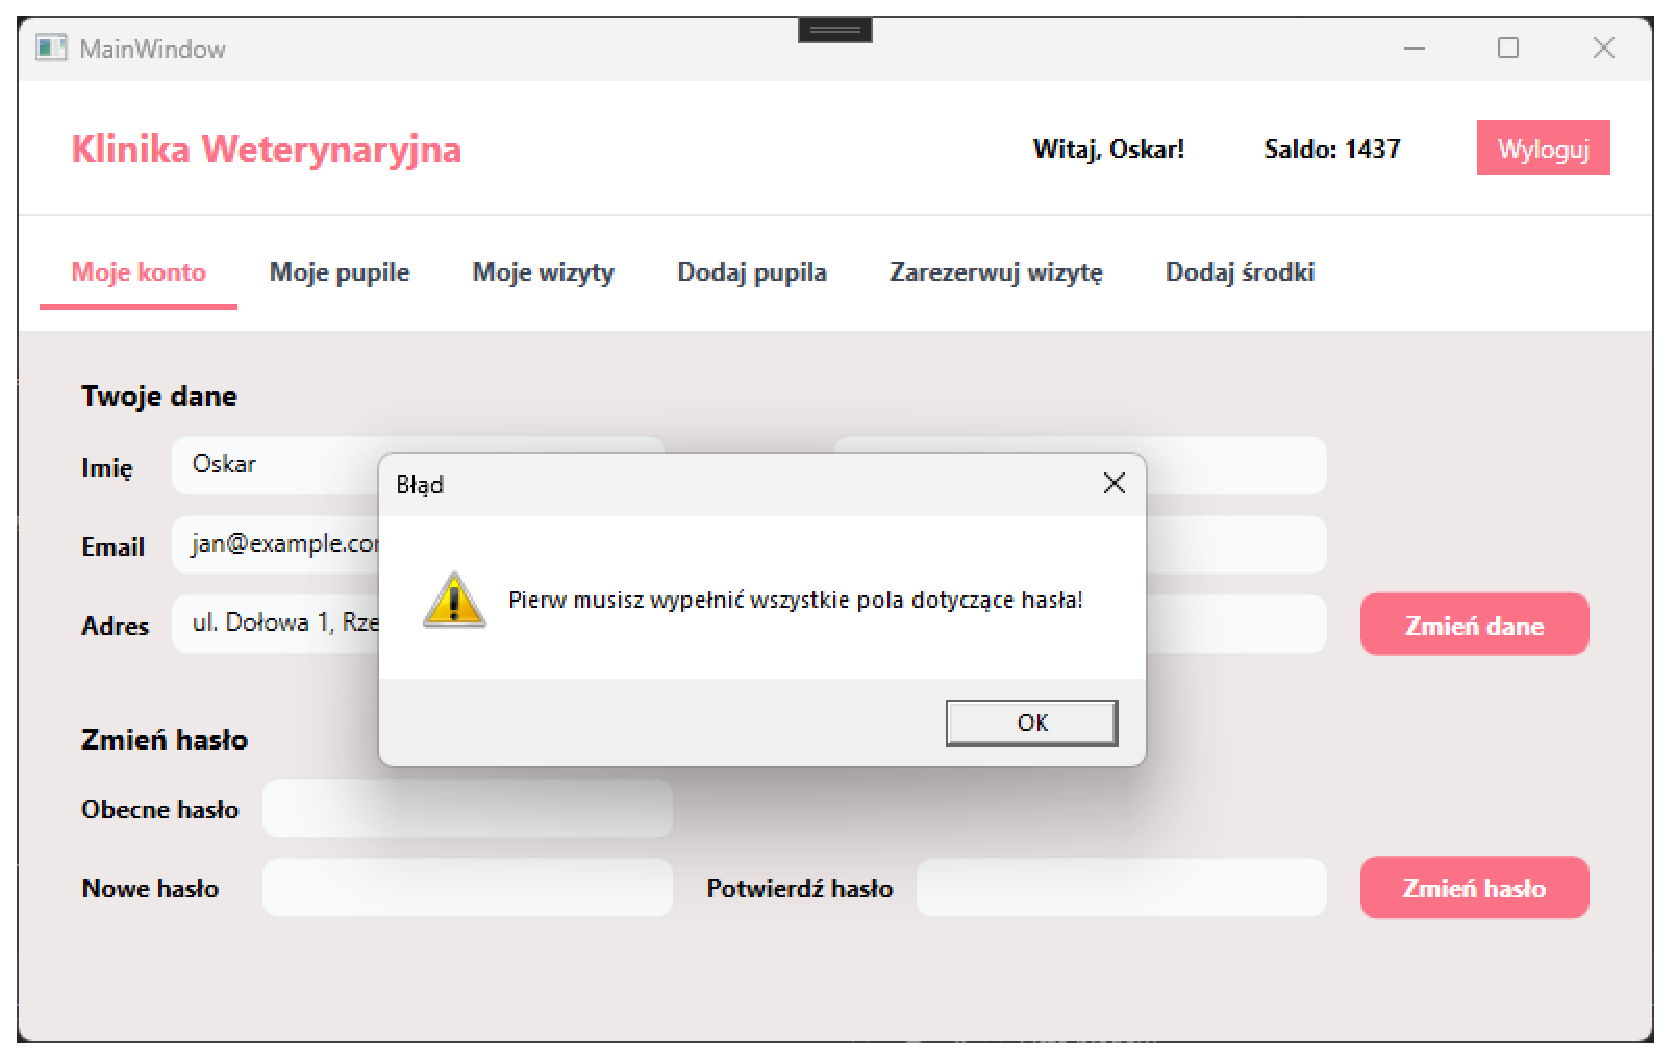
\includegraphics[width=0.9\linewidth]{figures/Uzytkownik/fig_014.eps}
\caption{Komunikat błędu przy niewypełnionych polach zmiany hasła.\label{fig14}}
\end{figure}

Aplikacja weryfikuje również poprawność obecnego hasła jeśli podane hasło nie zgadza się z aktualnym hasłem zapisanym
w systemie, wyświetlany jest komunikat błędu.

\begin{figure}[H]
\centering
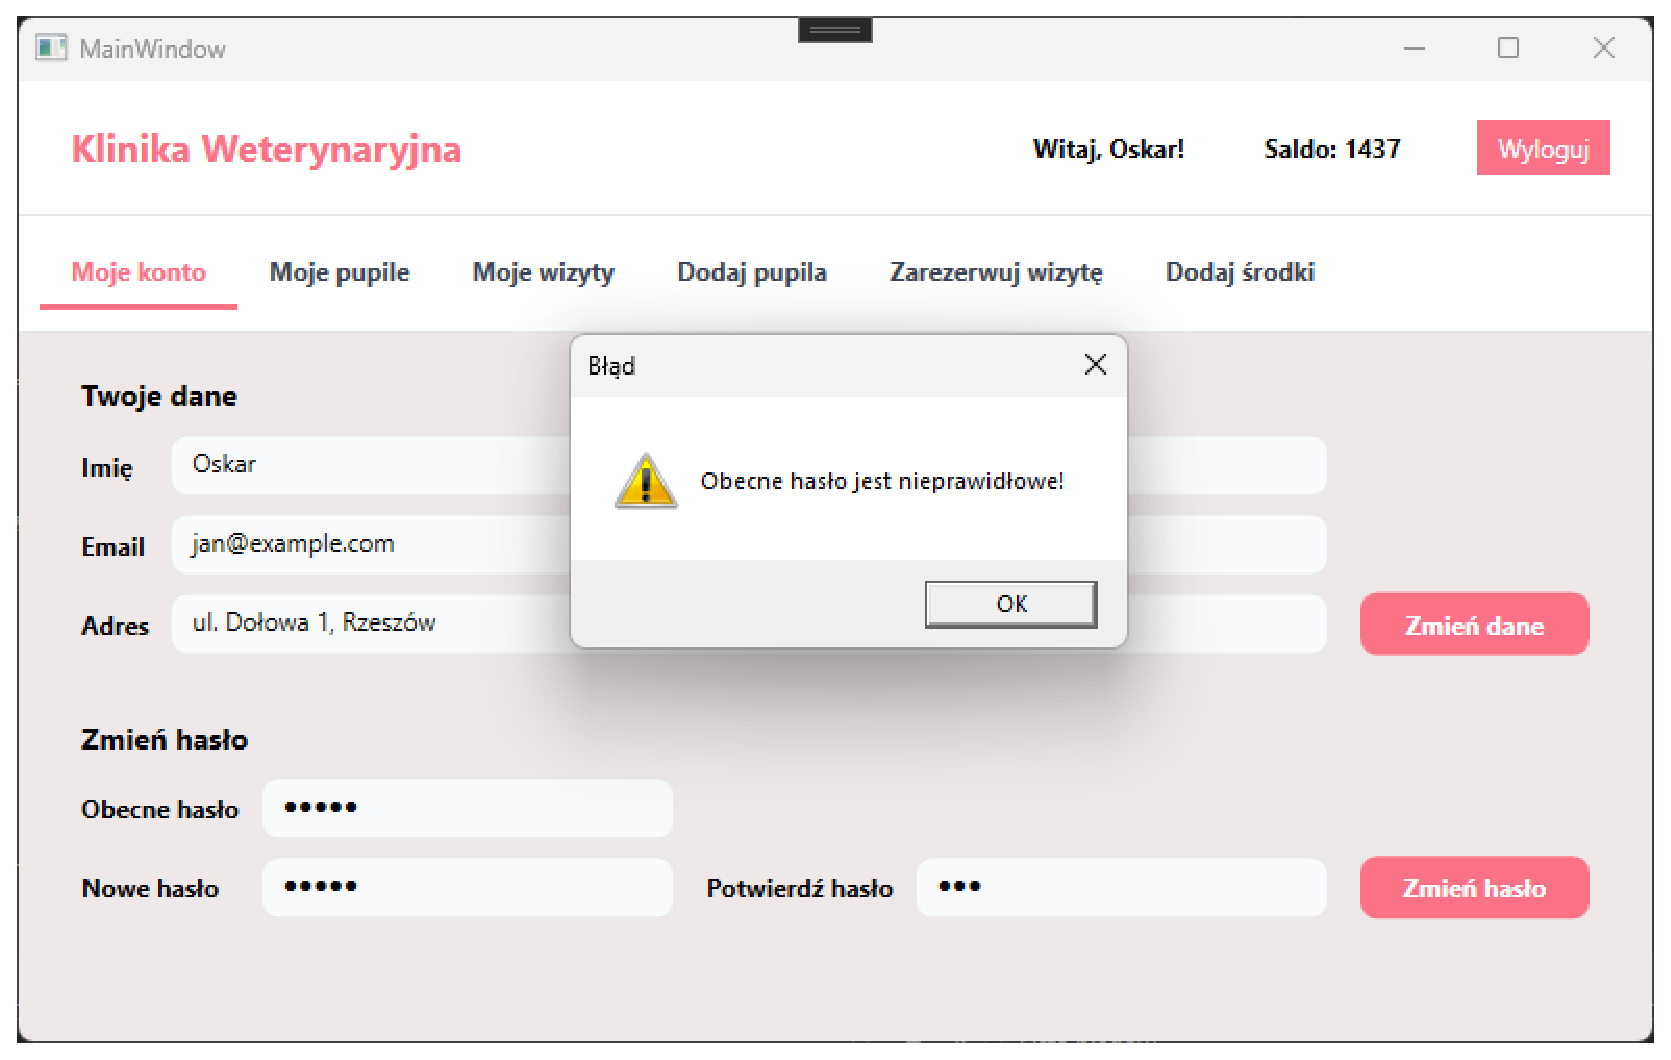
\includegraphics[width=0.9\linewidth]{figures/Uzytkownik/fig_015.eps}
\caption{Komunikat błędu przy nieprawidłowym obecnym haśle.\label{fig15}}
\end{figure}

Kolejnym etapem walidacji jest sprawdzenie zgodności nowego hasła z polem potwierdzającym oraz sprawdzenie czy hasło ma co najmniej 6 znaków. 
W przypadku niezgodności lub zbyt krótkiego hasła wyświetlane są odpowiednie komunikaty błędów.

\begin{figure}[H]
\centering
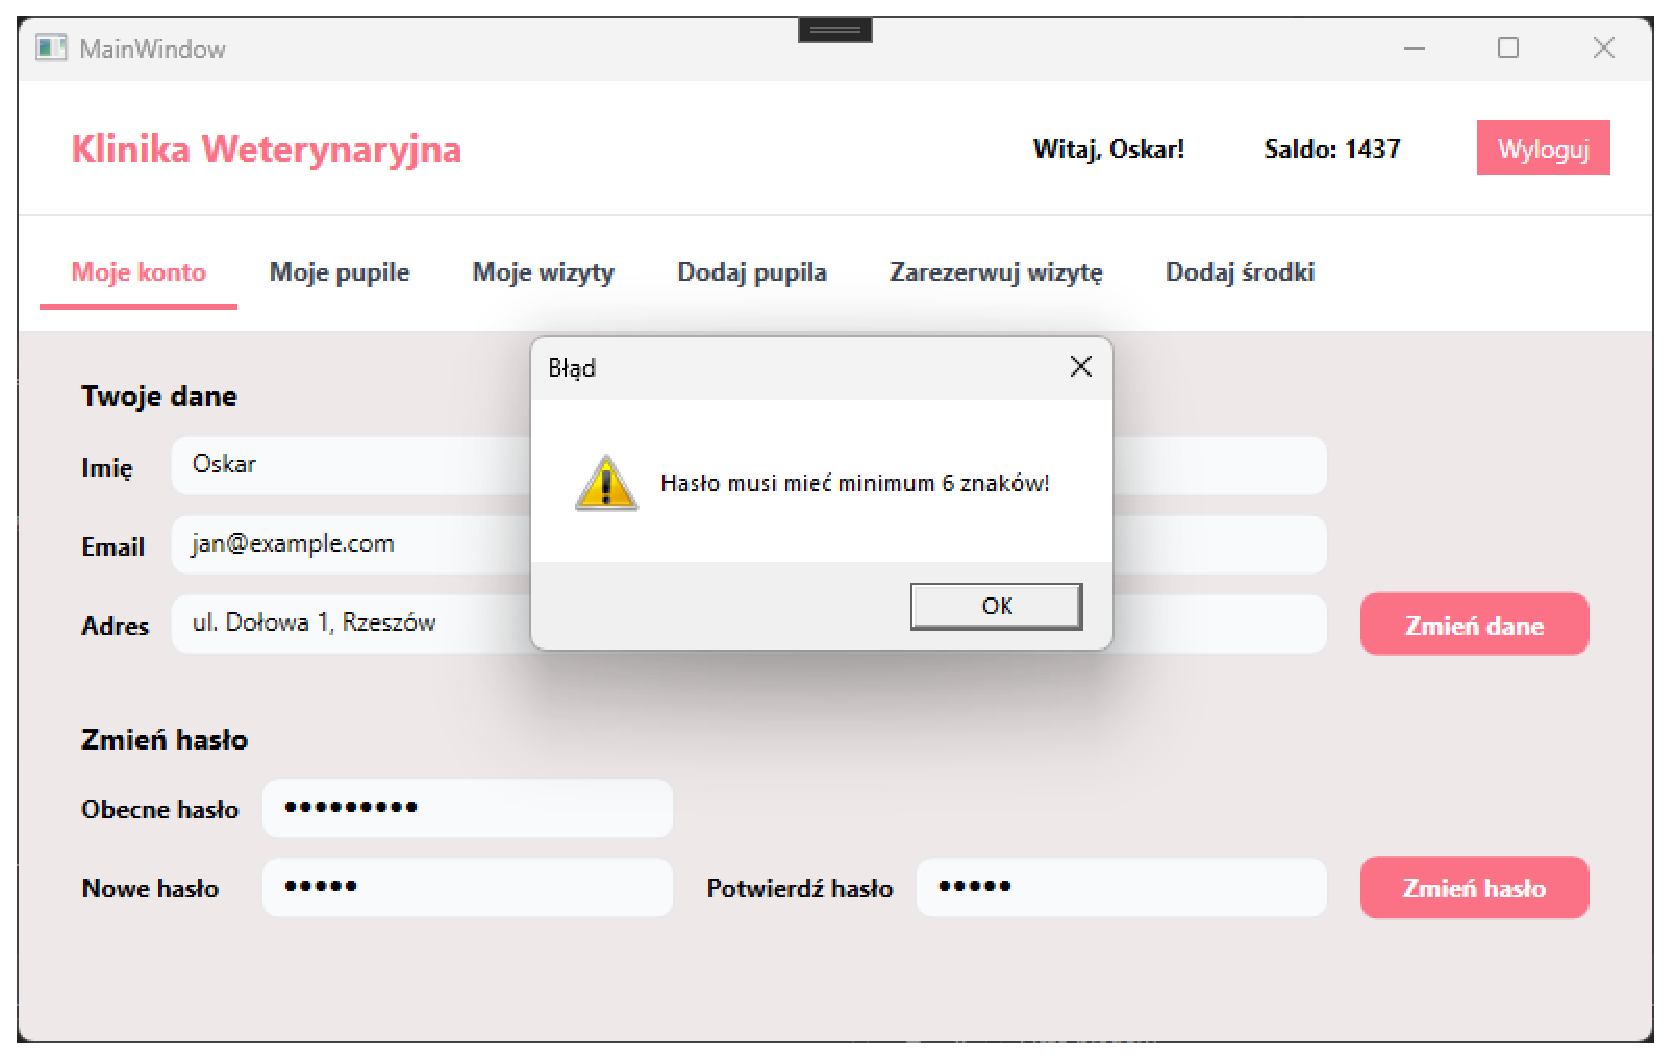
\includegraphics[width=0.9\linewidth]{figures/Uzytkownik/fig_016.eps}
\caption{Komunikat błędu przy niezgodności nowych haseł.\label{fig16}}
\end{figure}

\begin{figure}[H]
\centering
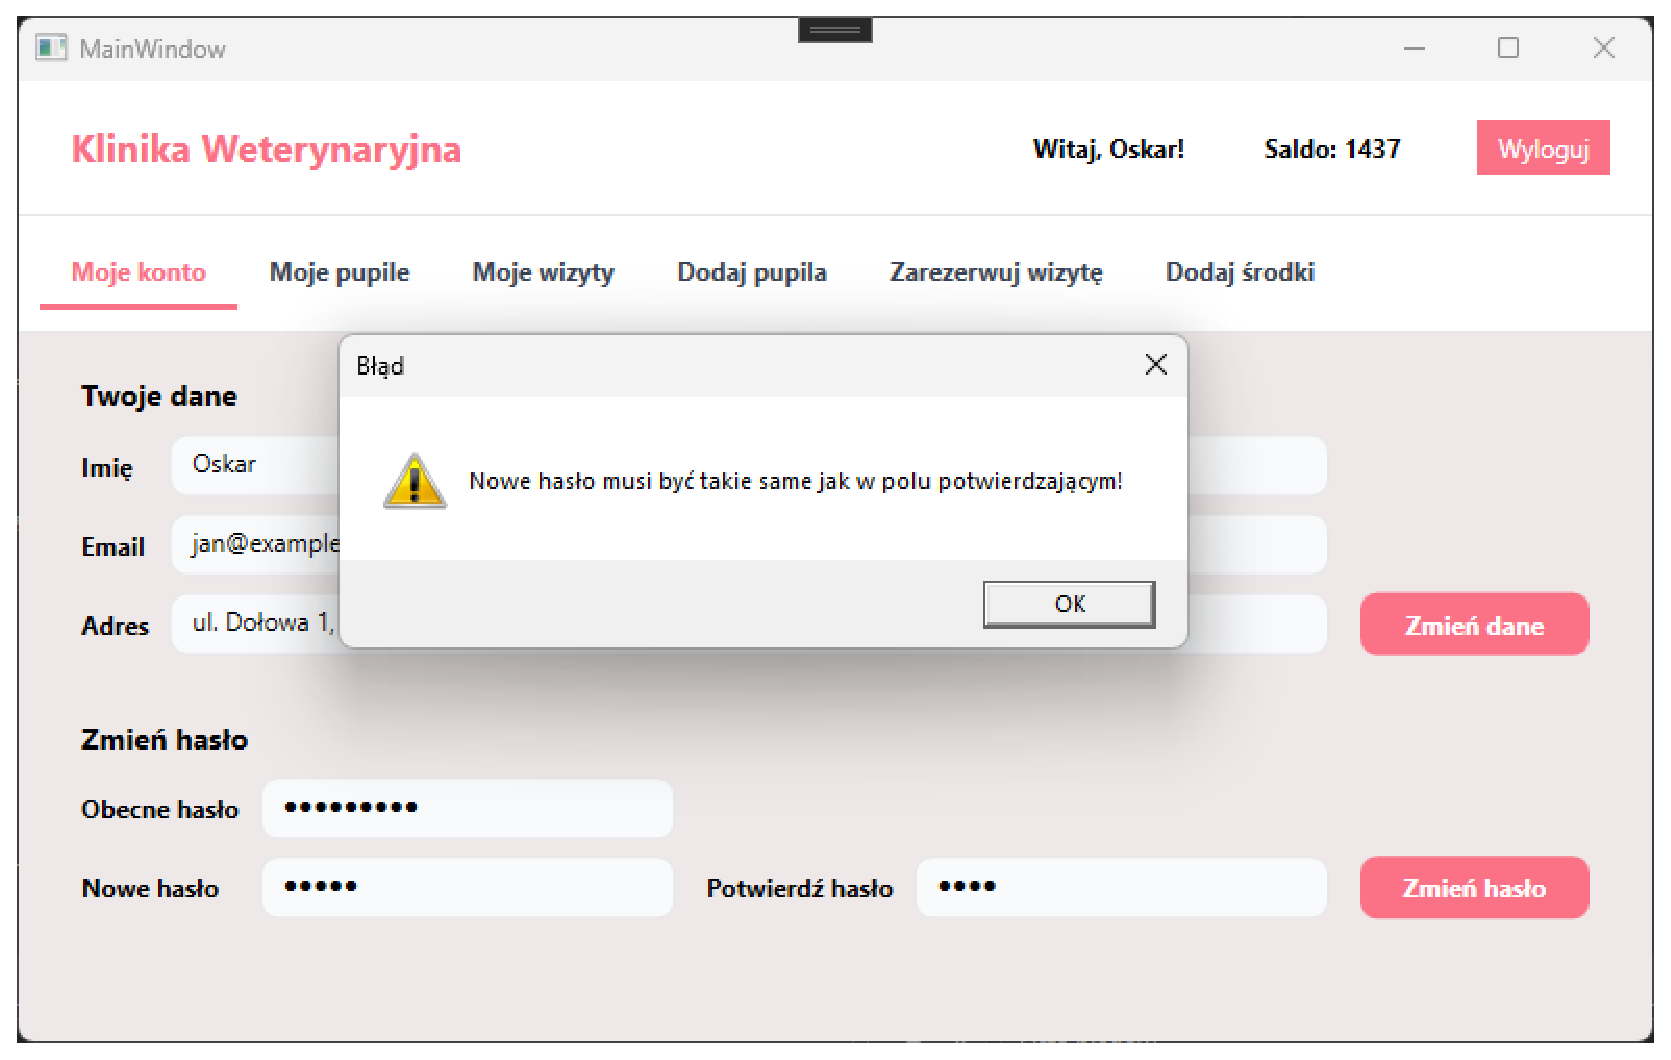
\includegraphics[width=0.9\linewidth]{figures/Uzytkownik/fig_017.eps}
\caption{Komunikat błędu przy haśle krótszym niż 6 znaków.\label{fig17}}
\end{figure}

\textbf{Zakładka "Moje pupile"}

Zakładka "Moje pupile" wyświetla listę wszystkich pupili przypisanych do zalogowanego użytkownika. Dla każdego pupila 
prezentowane są informacje takie jak imię, gatunek, rasa, wiek oraz płeć. Przy każdym pupilu dostępne 
dwa przyciski: Edytuj wiek umożliwiający zmianę wieku pupila oraz Usuń umożliwiający usunięcie pupila z systemu.

\begin{figure}[H]
\centering
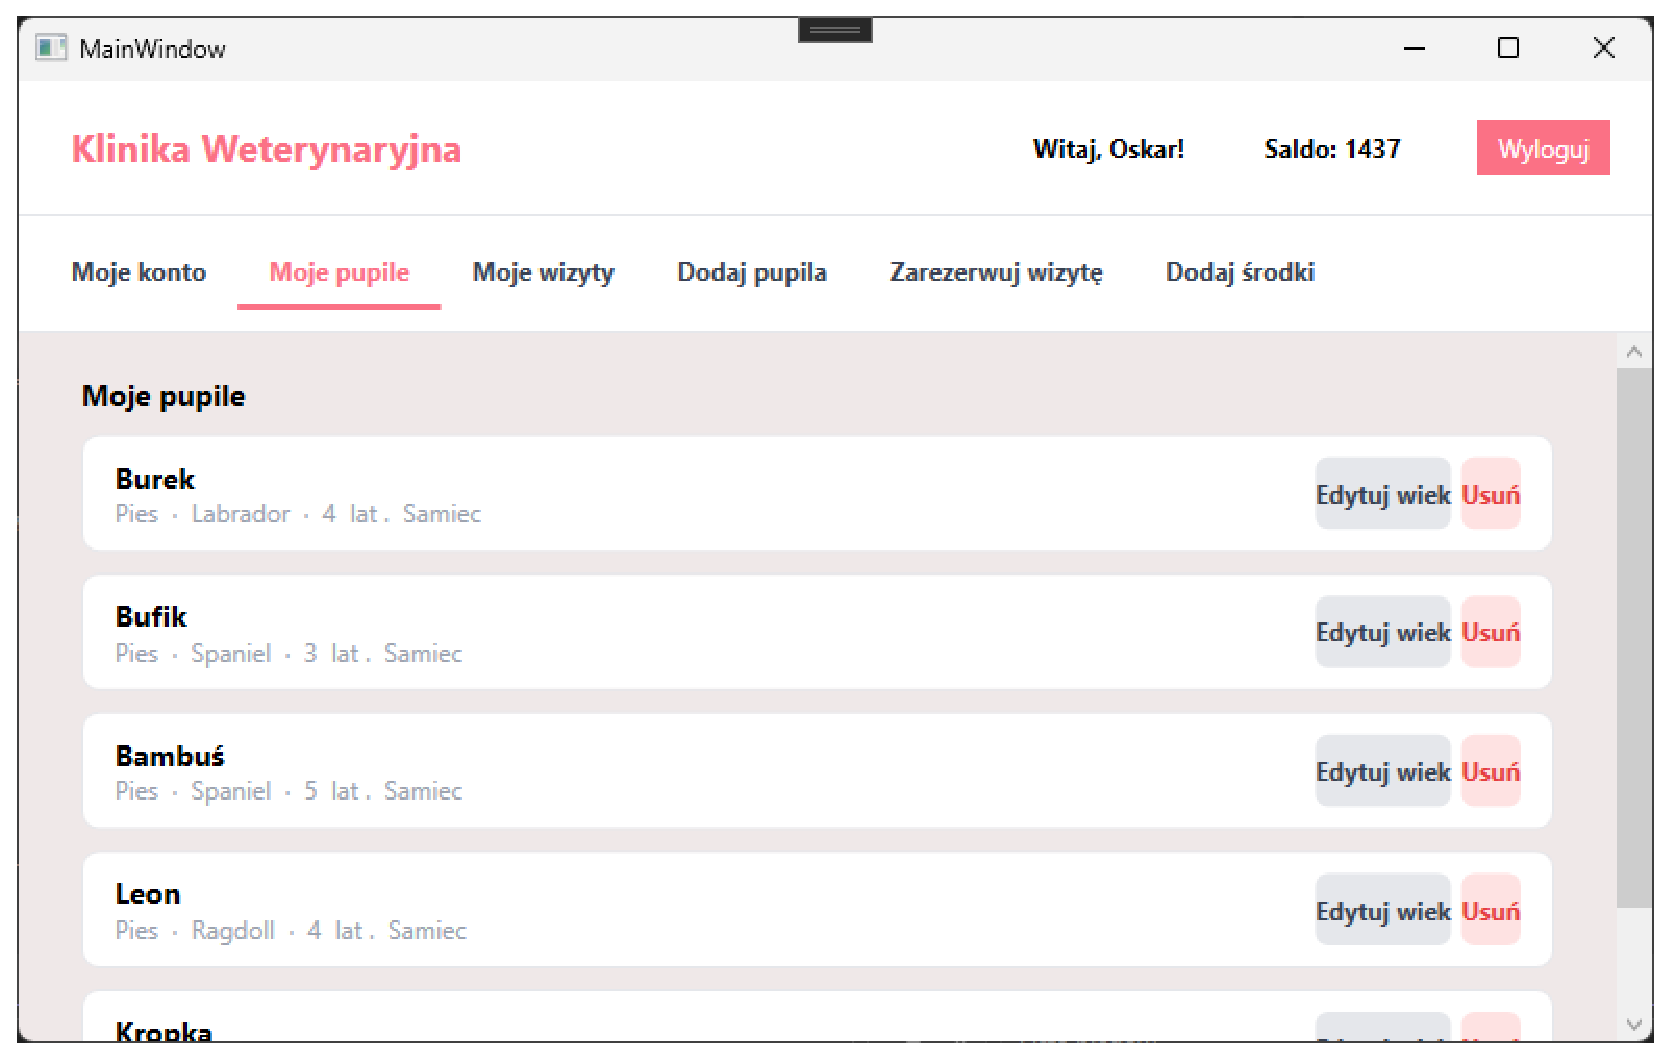
\includegraphics[width=0.9\linewidth]{figures/Uzytkownik/fig_018.eps}
\caption{Widok zakładki Moje pupile.\label{fig18}}
\end{figure}

Po kliknięciu przycisku Edytuj wiek otwierane jest okno dialogowe z polem tekstowym, w którym użytkownik może wprowadzić nowy wiek pupila. 
Zmiana zostaje zapisana po kliknięciu przycisku Zapisz.

\begin{figure}[H]
\centering
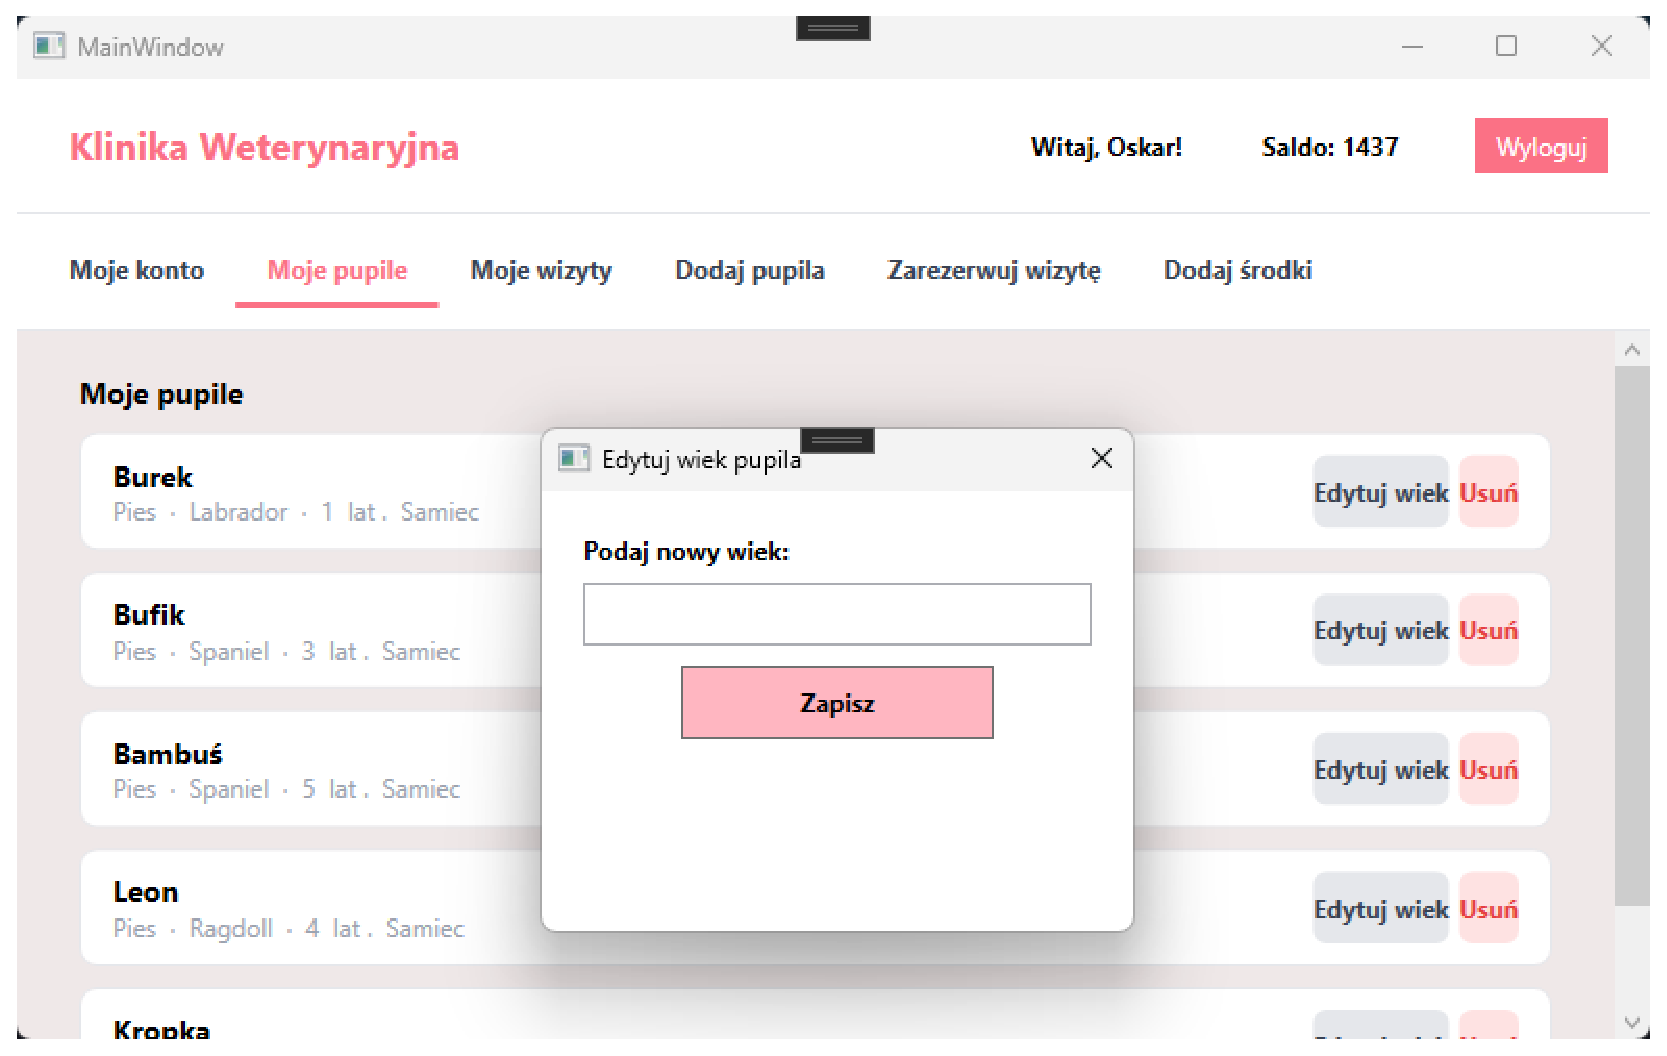
\includegraphics[width=0.9\linewidth]{figures/Uzytkownik/fig_019.eps}
\caption{Okno dialogowe edycji wieku pupila.\label{fig19}}
\end{figure}

W przypadku podania nieprawidłowej wartości wieku aplikacja wyświetla komunikat błędu informujący o konieczności podania prawidłowej wartości.

\begin{figure}[H]
\centering
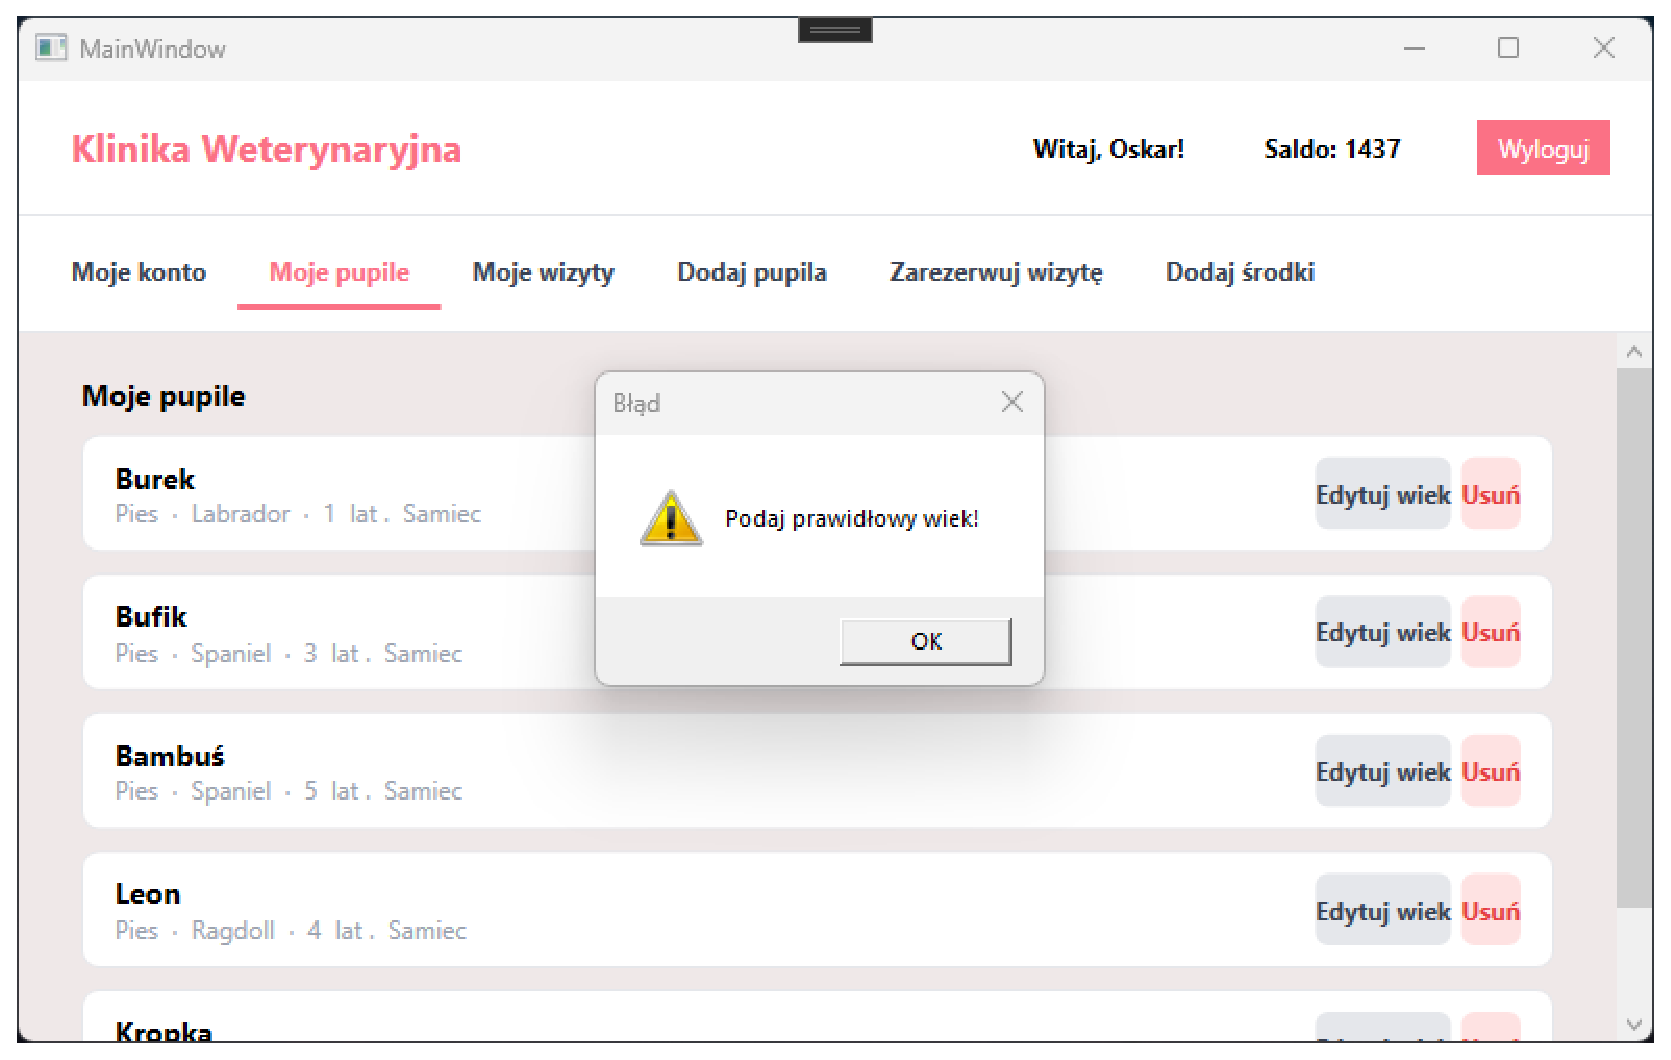
\includegraphics[width=0.9\linewidth]{figures/Uzytkownik/fig_020.eps}
\caption{Komunikat błędu przy nieprawidłowym wieku pupila.\label{fig20}}
\end{figure}

Po kliknięciu przycisku Usuń aplikacja wyświetla okno dialogowe z prośbą o potwierdzenie operacji. 
Po potwierdzeniu pupil zostaje usunięty z systemu wraz z jego rezerwacjami, a lista pupili jest automatycznie odświeżana.

\begin{figure}[H]
\centering
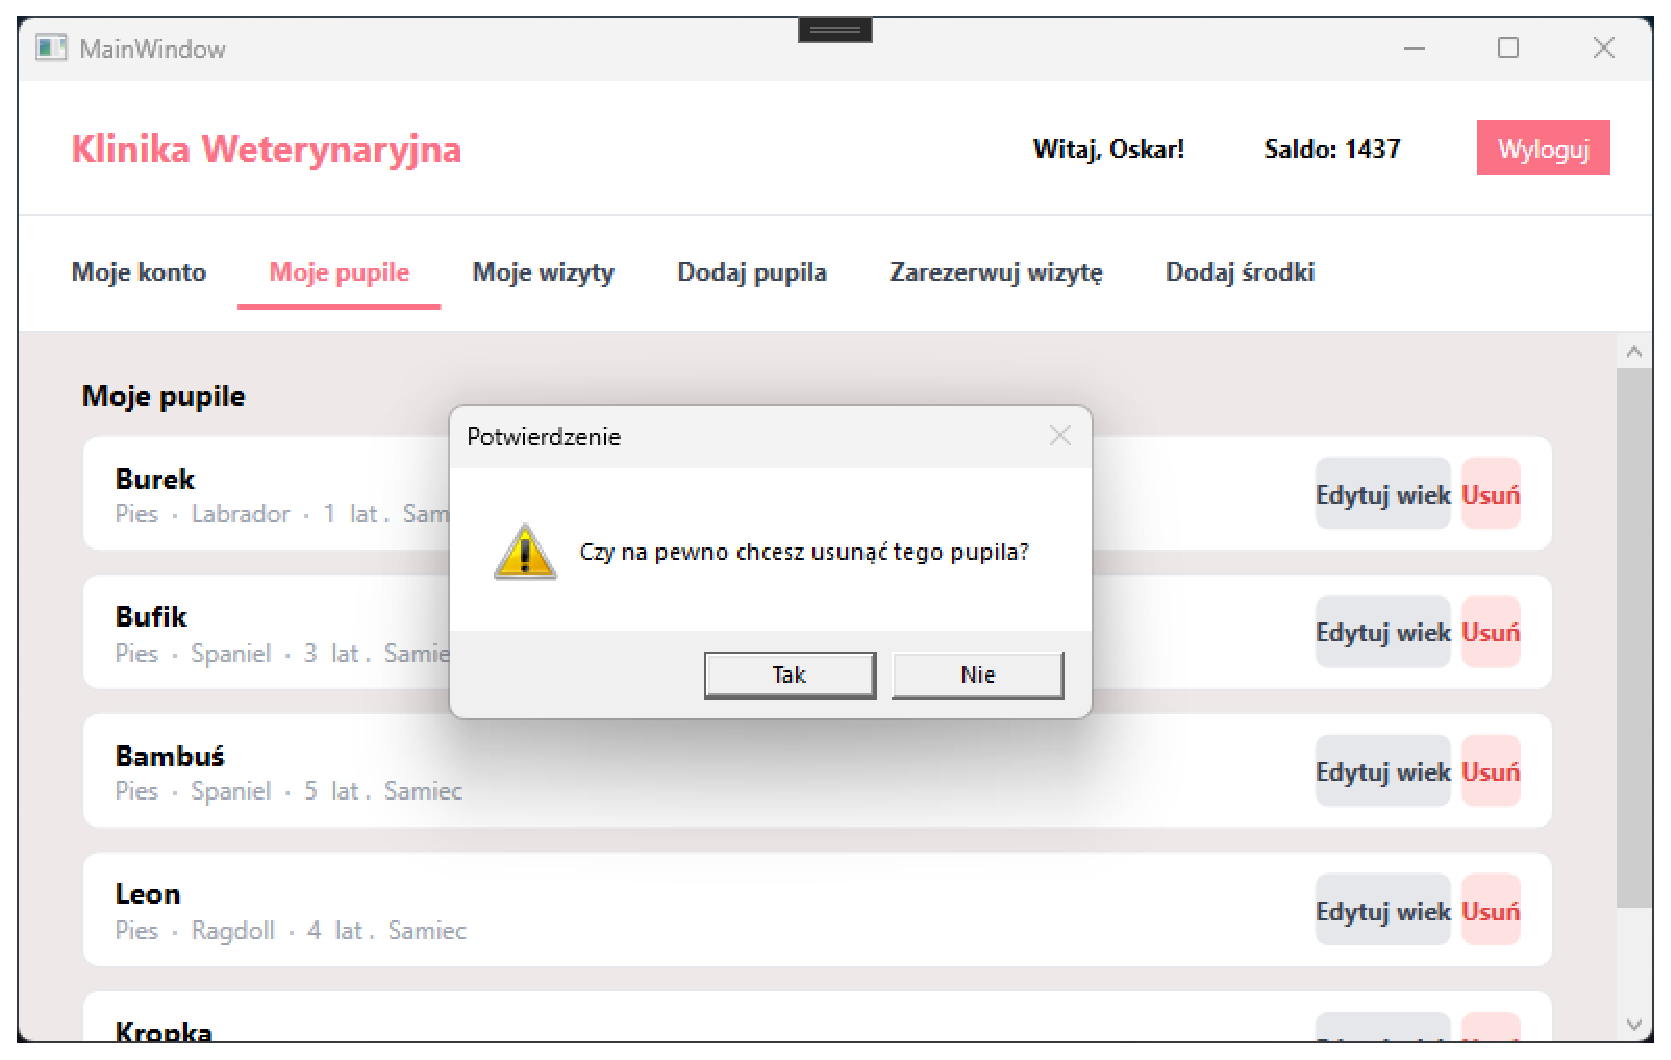
\includegraphics[width=0.9\linewidth]{figures/Uzytkownik/fig_021.eps}
\caption{Okno potwierdzenia usunięcia pupila.\label{fig21}}
\end{figure}

\textbf{Zakładka "Moje wizyty"}

Zakładka "Moje Wizyty" wyświetla historię wszystkich rezerwacji wizyt zalogowanego użytkownika. Dla każdej wizyty prezentowane 
są informacje takie jak nazwa zabiegu, imię pupila, data, godziny wizyty oraz imię i nazwisko weterynarza. Każda wizyta oznaczona 
jest kolorowym znacznikiem statusu: zielonym dla wizyt zarezerwowanych, szarym dla anulowanych oraz ciemnozielonym dla zrealizowanych. 
Przy każdej wizycie dostępny jest przycisk Anuluj umożliwiający anulowanie rezerwacji.

\begin{figure}[H]
\centering
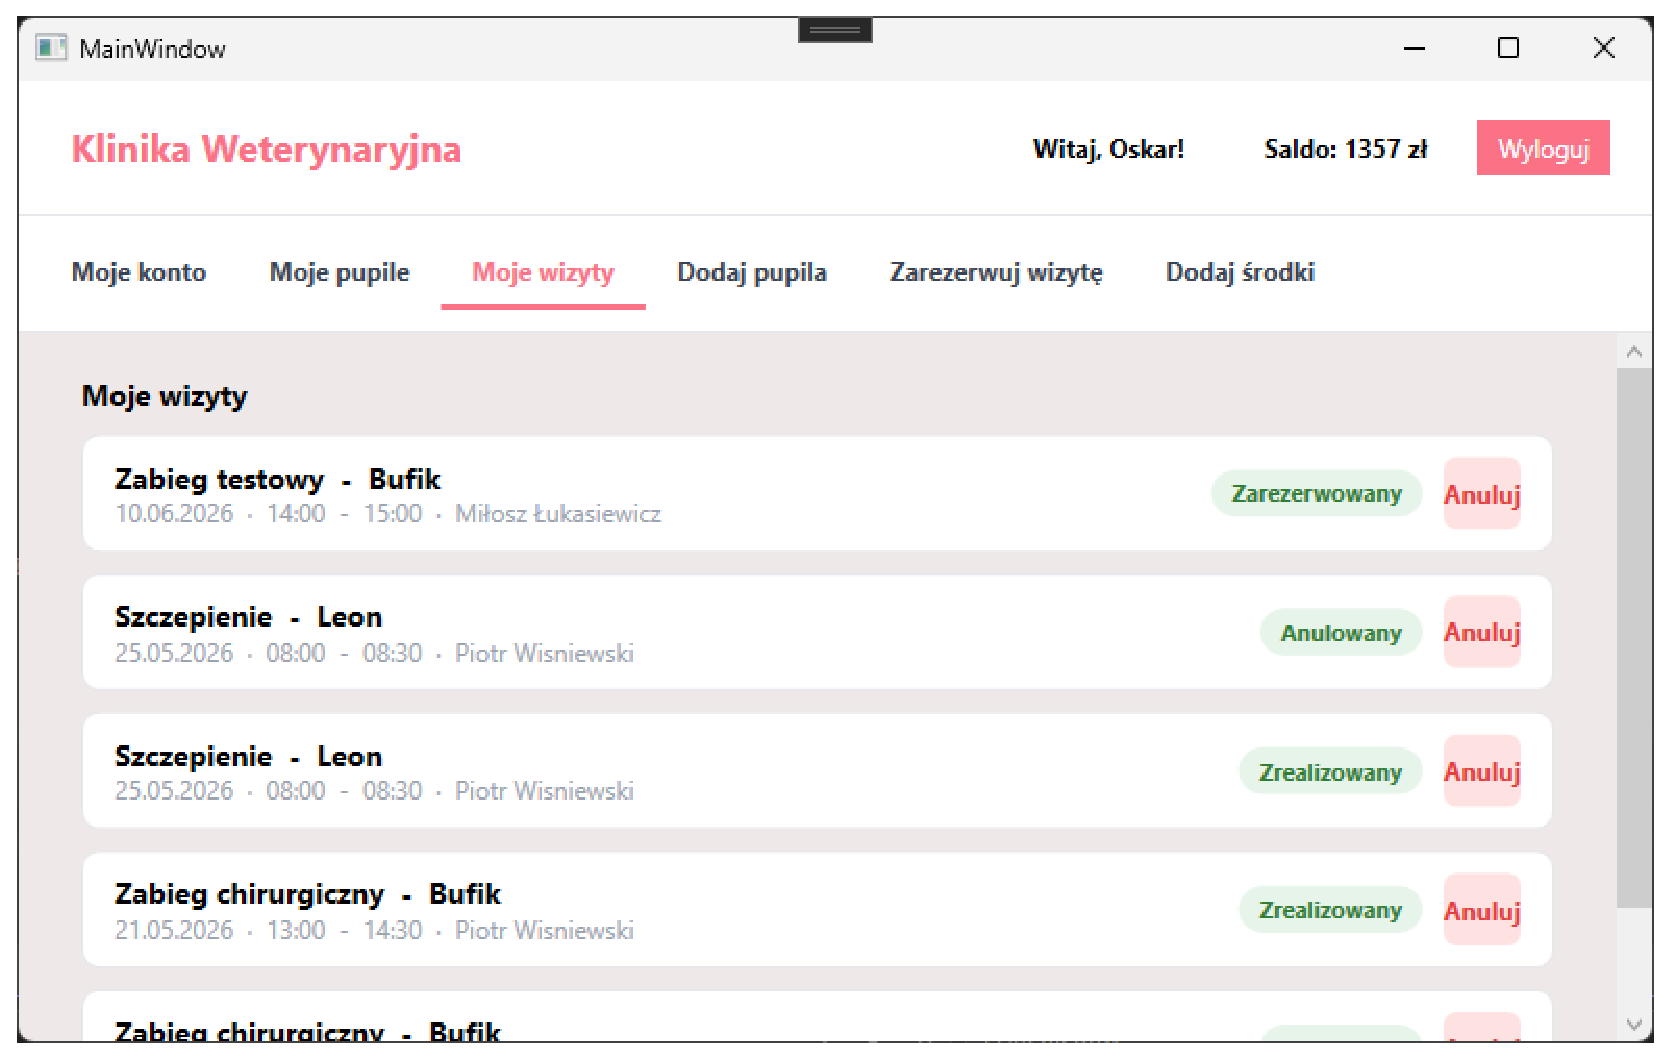
\includegraphics[width=0.9\linewidth]{figures/Uzytkownik/fig_022.eps}
\caption{Widok zakładki Moje wizyty.\label{fig22}}
\end{figure}

Po kliknięciu przycisku Anuluj aplikacja wyświetla okno dialogowe z prośbą o potwierdzenie operacji. 
Po potwierdzeniu status wizyty zostaje zmieniony na Anulowany, a lista wizyt jest automatycznie odświeżana.

\begin{figure}[H]
\centering
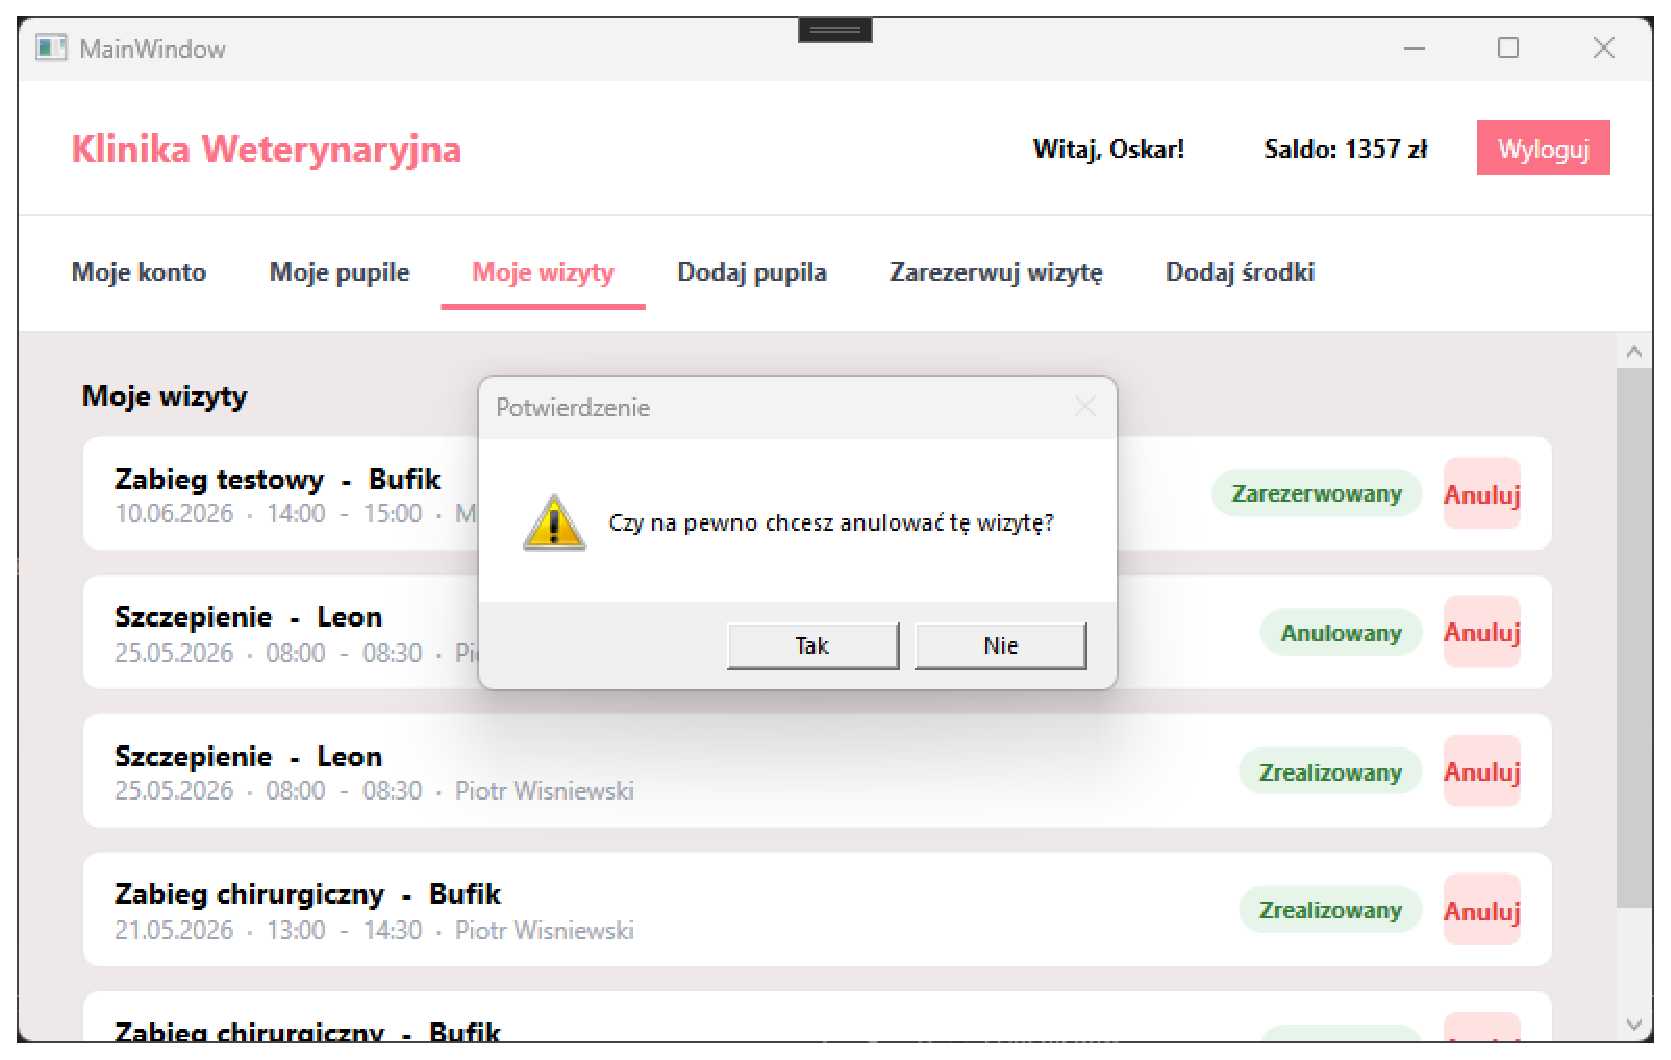
\includegraphics[width=0.9\linewidth]{figures/Uzytkownik/fig_023.eps}
\caption{Okno potwierdzenia anulowania wizyty.\label{fig23}}
\end{figure}

\textbf{Okno "Dodaj pupila"}

Okno "Dodaj pupila" otwierane jest po kliknięciu przycisku Dodaj pupila w pasku nawigacyjnym. Formularz zawiera pola: imię, 
gatunek (lista rozwijana z opcjami Pies i Kot), rasa, wiek w latach oraz płeć (lista rozwijana z opcjami Samiec i Samica). 
Po wypełnieniu formularza i kliknięciu przycisku Dodaj Pupila aplikacja przeprowadza walidację wprowadzonych danych.

\begin{figure}[H]
\centering
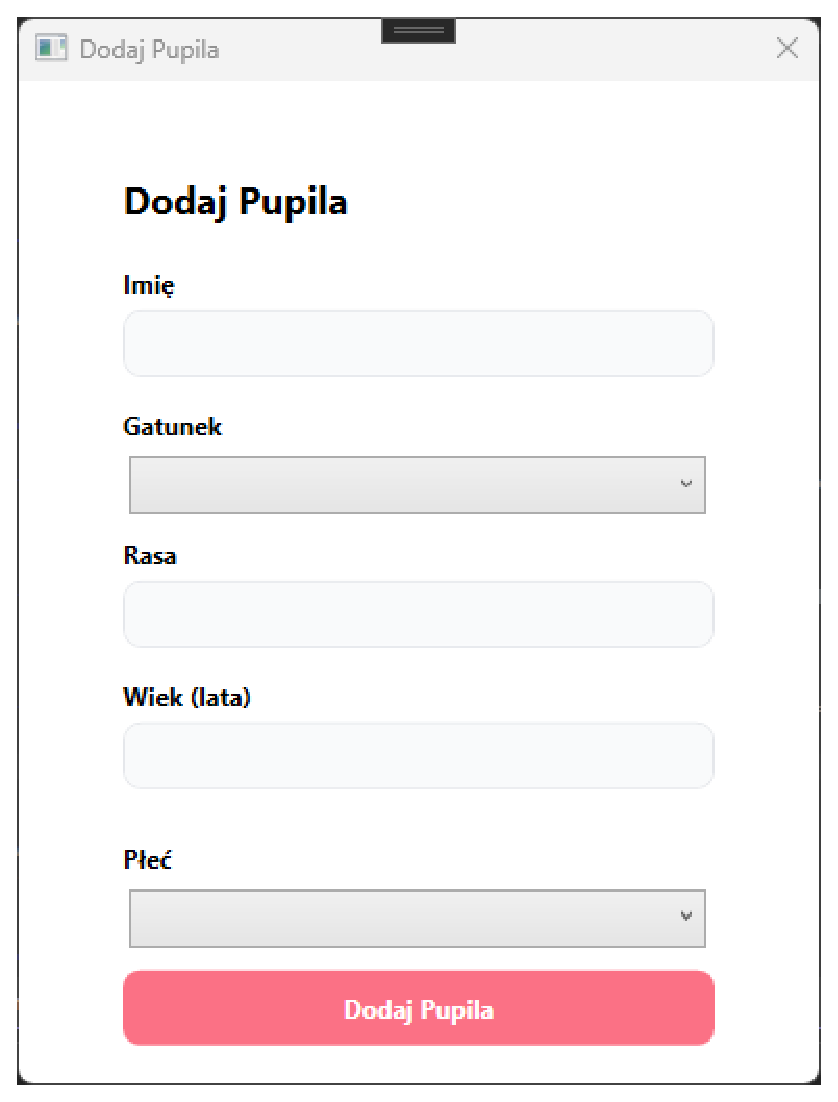
\includegraphics[width=0.7\linewidth]{figures/Uzytkownik/fig_024.eps}
\caption{Widok okna Dodaj pupila.\label{fig24}}
\end{figure}

W przypadku gdy użytkownik nie wypełni wszystkich pól formularza, aplikacja wyświetla komunikat błędu informujący o konieczności uzupełnienia wszystkich pól.

\begin{figure}[H]
\centering
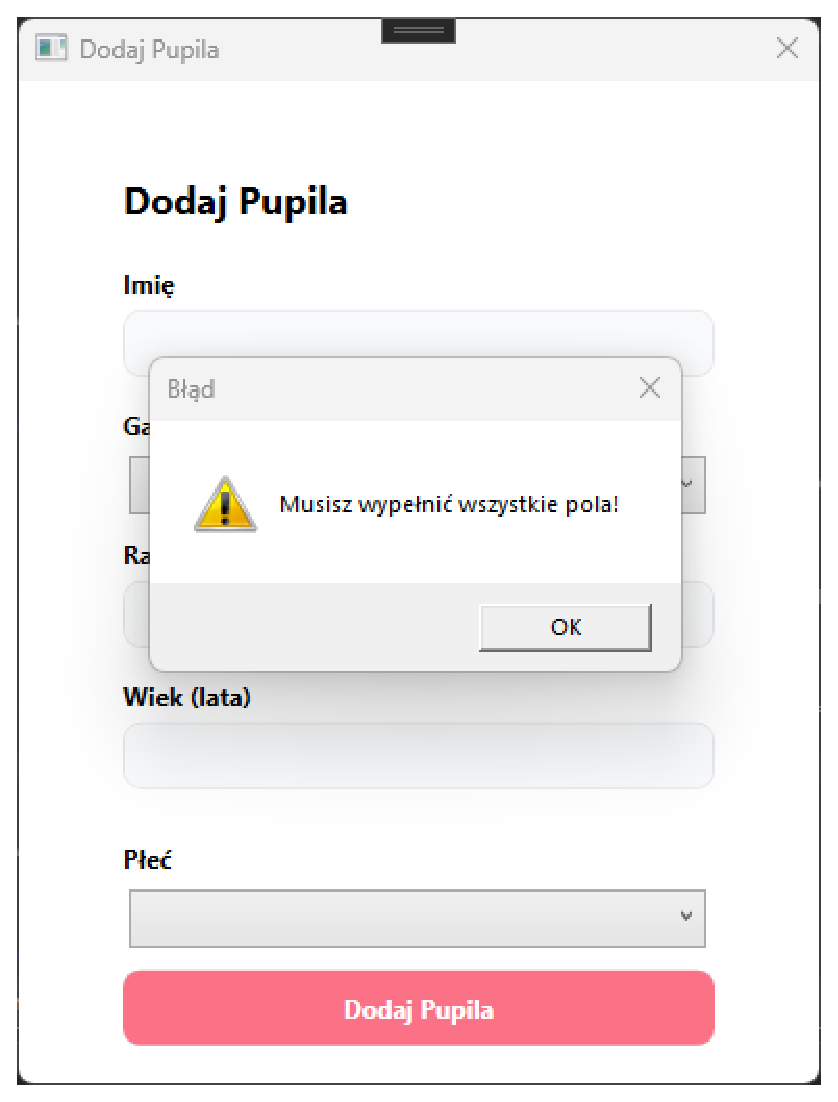
\includegraphics[width=0.7\linewidth]{figures/Uzytkownik/fig_025.eps}
\caption{Komunikat błędu przy niewypełnionych polach formularza.\label{fig25}}
\end{figure}

Po poprawnym wypełnieniu wszystkich pól i kliknięciu przycisku Dodaj Pupila nowy pupil zostaje zapisany w bazie danych i 
przypisany do zalogowanego użytkownika. Aplikacja wyświetla komunikat potwierdzający pomyślne dodanie pupila, a okno zostaje zamknięte.

\begin{figure}[H]
\centering
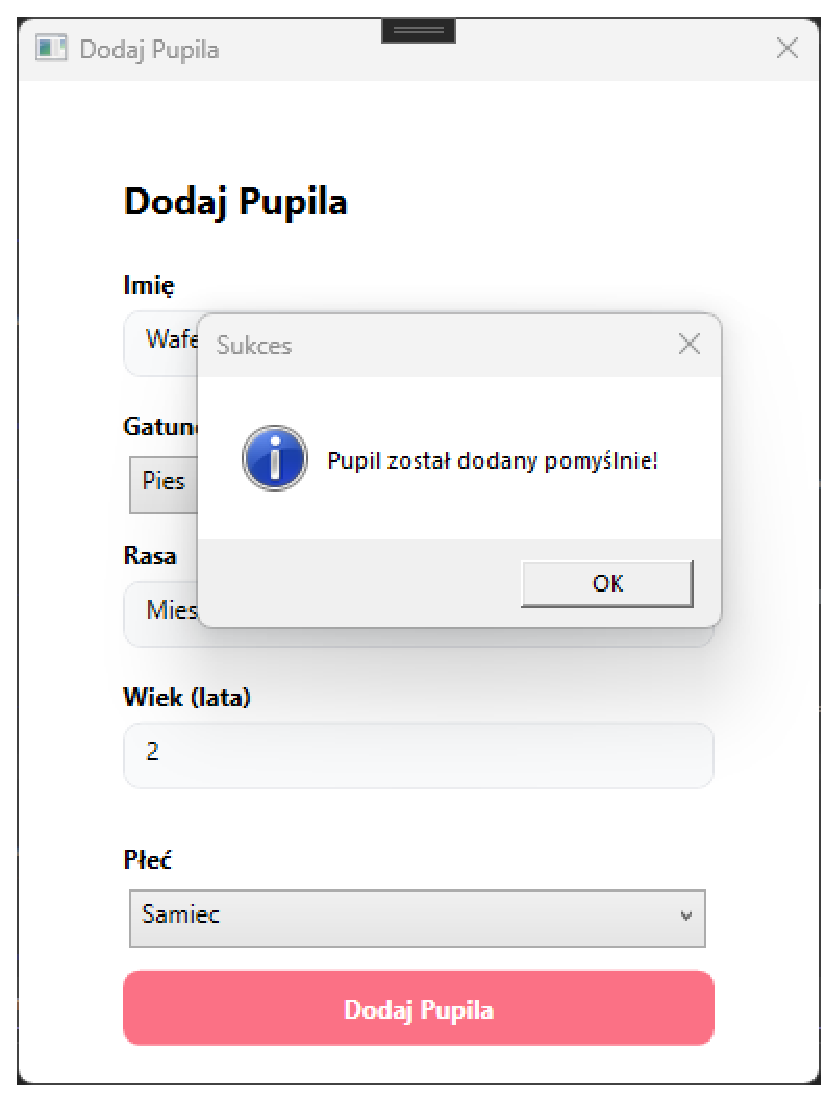
\includegraphics[width=0.7\linewidth]{figures/Uzytkownik/fig_026.eps}
\caption{Komunikat potwierdzający pomyślne dodanie pupila.\label{fig26}}
\end{figure}

\textbf{Okno "Nowa rezerwacja"}

Okno "Nowa rezerwacja" otwierane jest po kliknięciu przycisku Zarezerwuj wizytę w pasku nawigacyjnym. Proces rezerwacji podzielony jest na trzy kroki. 
W pierwszym kroku użytkownik wybiera pupila z listy rozwijanej oraz zabieg z listy dostępnych zabiegów. Dla każdego zabiegu wyświetlany jest czas trwania oraz cena.

\begin{figure}[H]
\centering
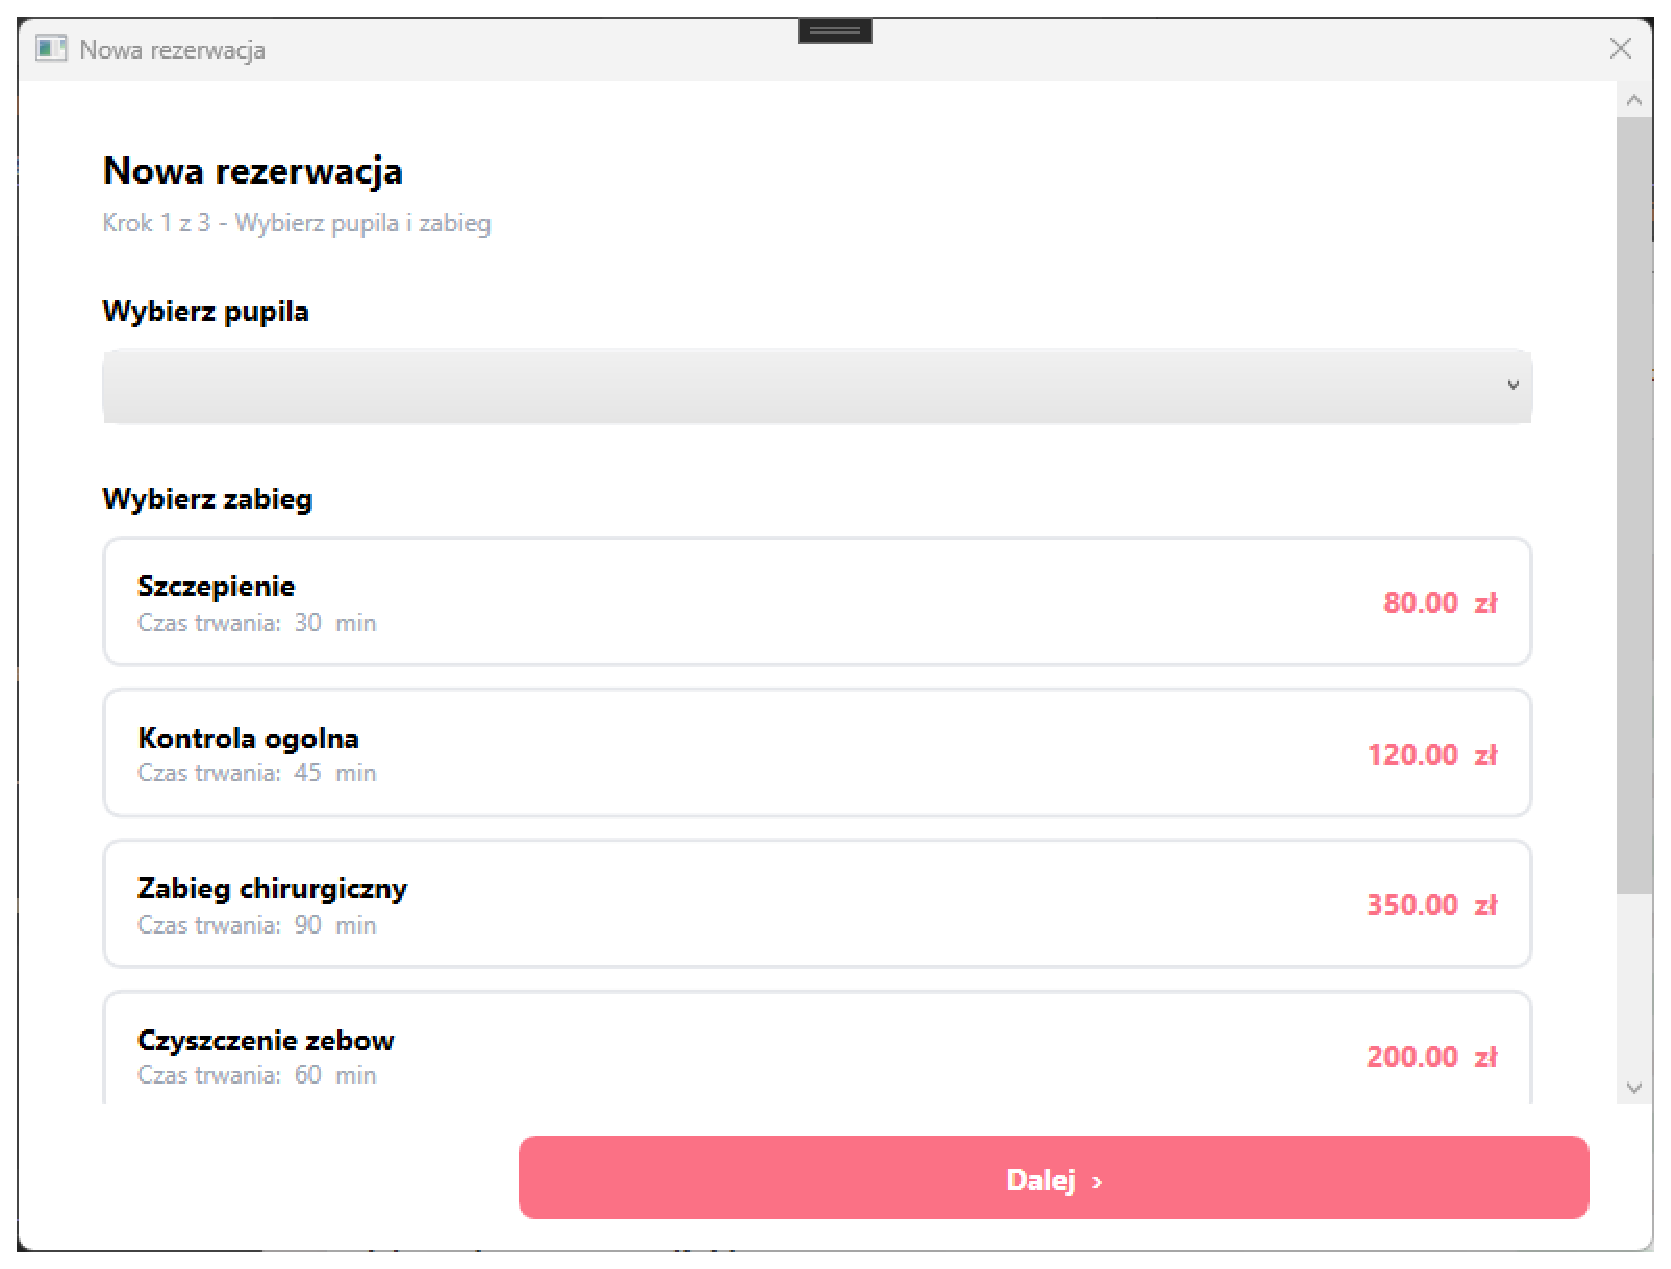
\includegraphics[width=0.9\linewidth]{figures/Uzytkownik/fig_027.eps}
\caption{Krok 1 - widok wyboru pupila i zabiegu.\label{fig27}}
\end{figure}

W przypadku gdy użytkownik nie wybierze pupila przed kliknięciem przycisku Dalej, aplikacja wyświetla komunikat błędu. Analogicznie, jeśli 
użytkownik nie wybierze zabiegu, wyświetlany jest odpowiedni komunikat.

\begin{figure}[H]
\centering
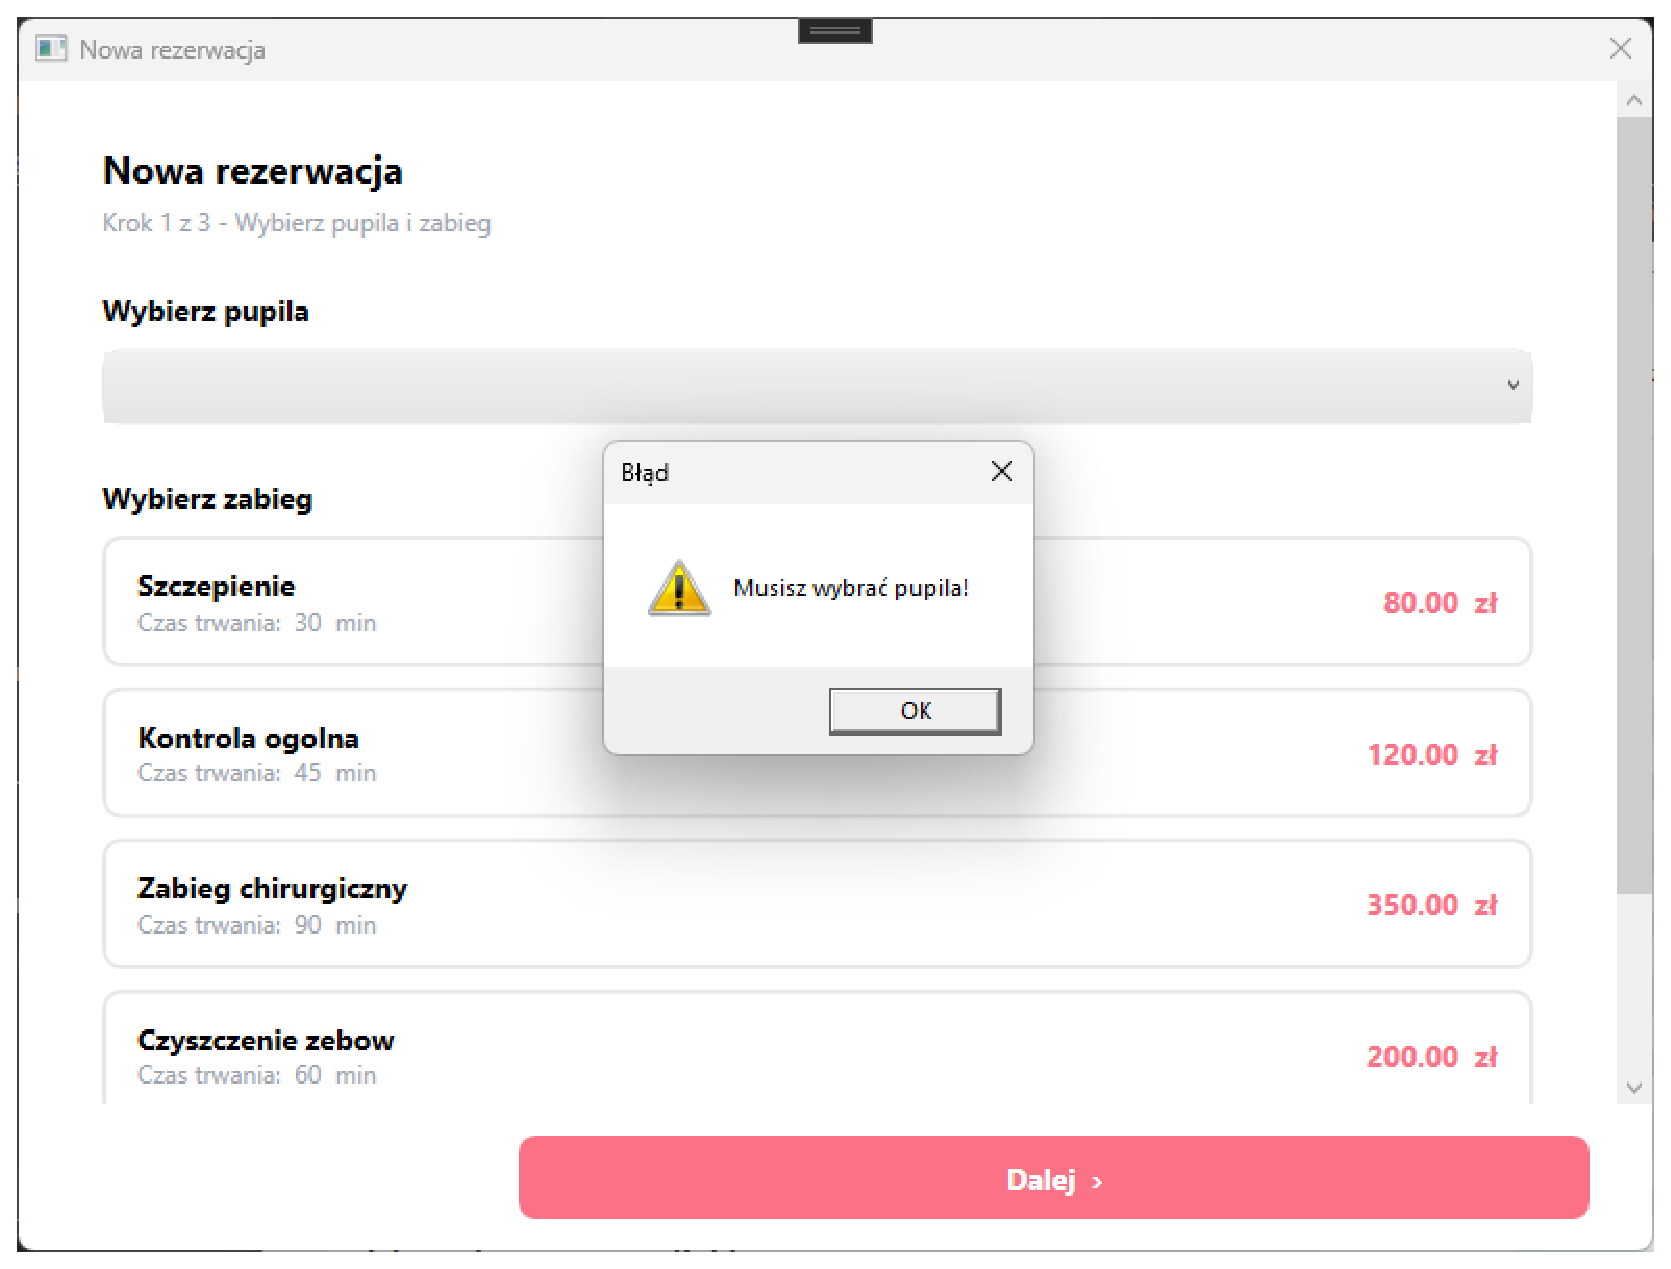
\includegraphics[width=0.9\linewidth]{figures/Uzytkownik/fig_028.eps}
\caption{Komunikat błędu przy braku wybranego pupila.\label{fig28}}
\end{figure}

\begin{figure}[H]
\centering
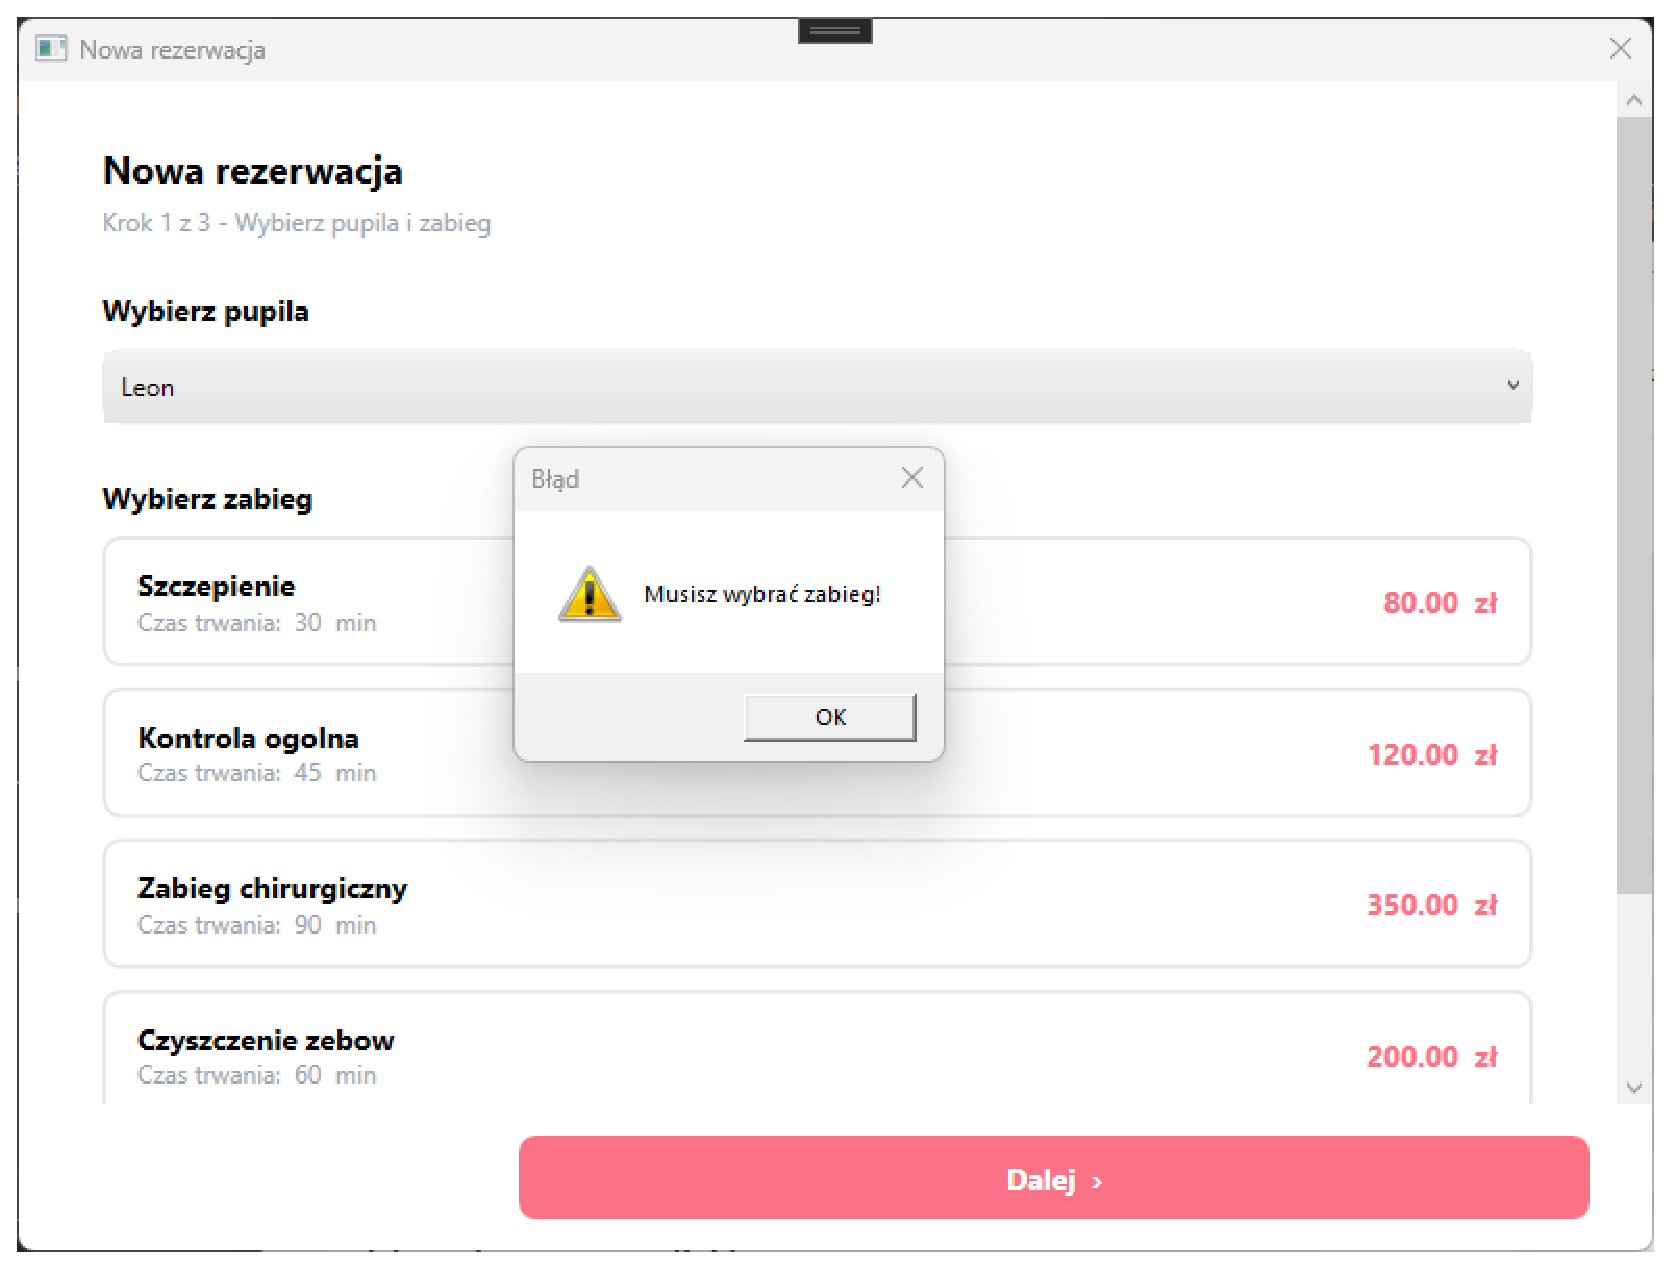
\includegraphics[width=0.9\linewidth]{figures/Uzytkownik/fig_029.eps}
\caption{Komunikat błędu przy braku wybranego zabiegu.\label{fig29}}
\end{figure}

W drugim kroku użytkownik wybiera weterynarza spośród tych, którzy wykonują wybrany zabieg. 
Dla każdego weterynarza wyświetlane jest imię, nazwisko oraz specjalizacja.

\begin{figure}[H]
\centering
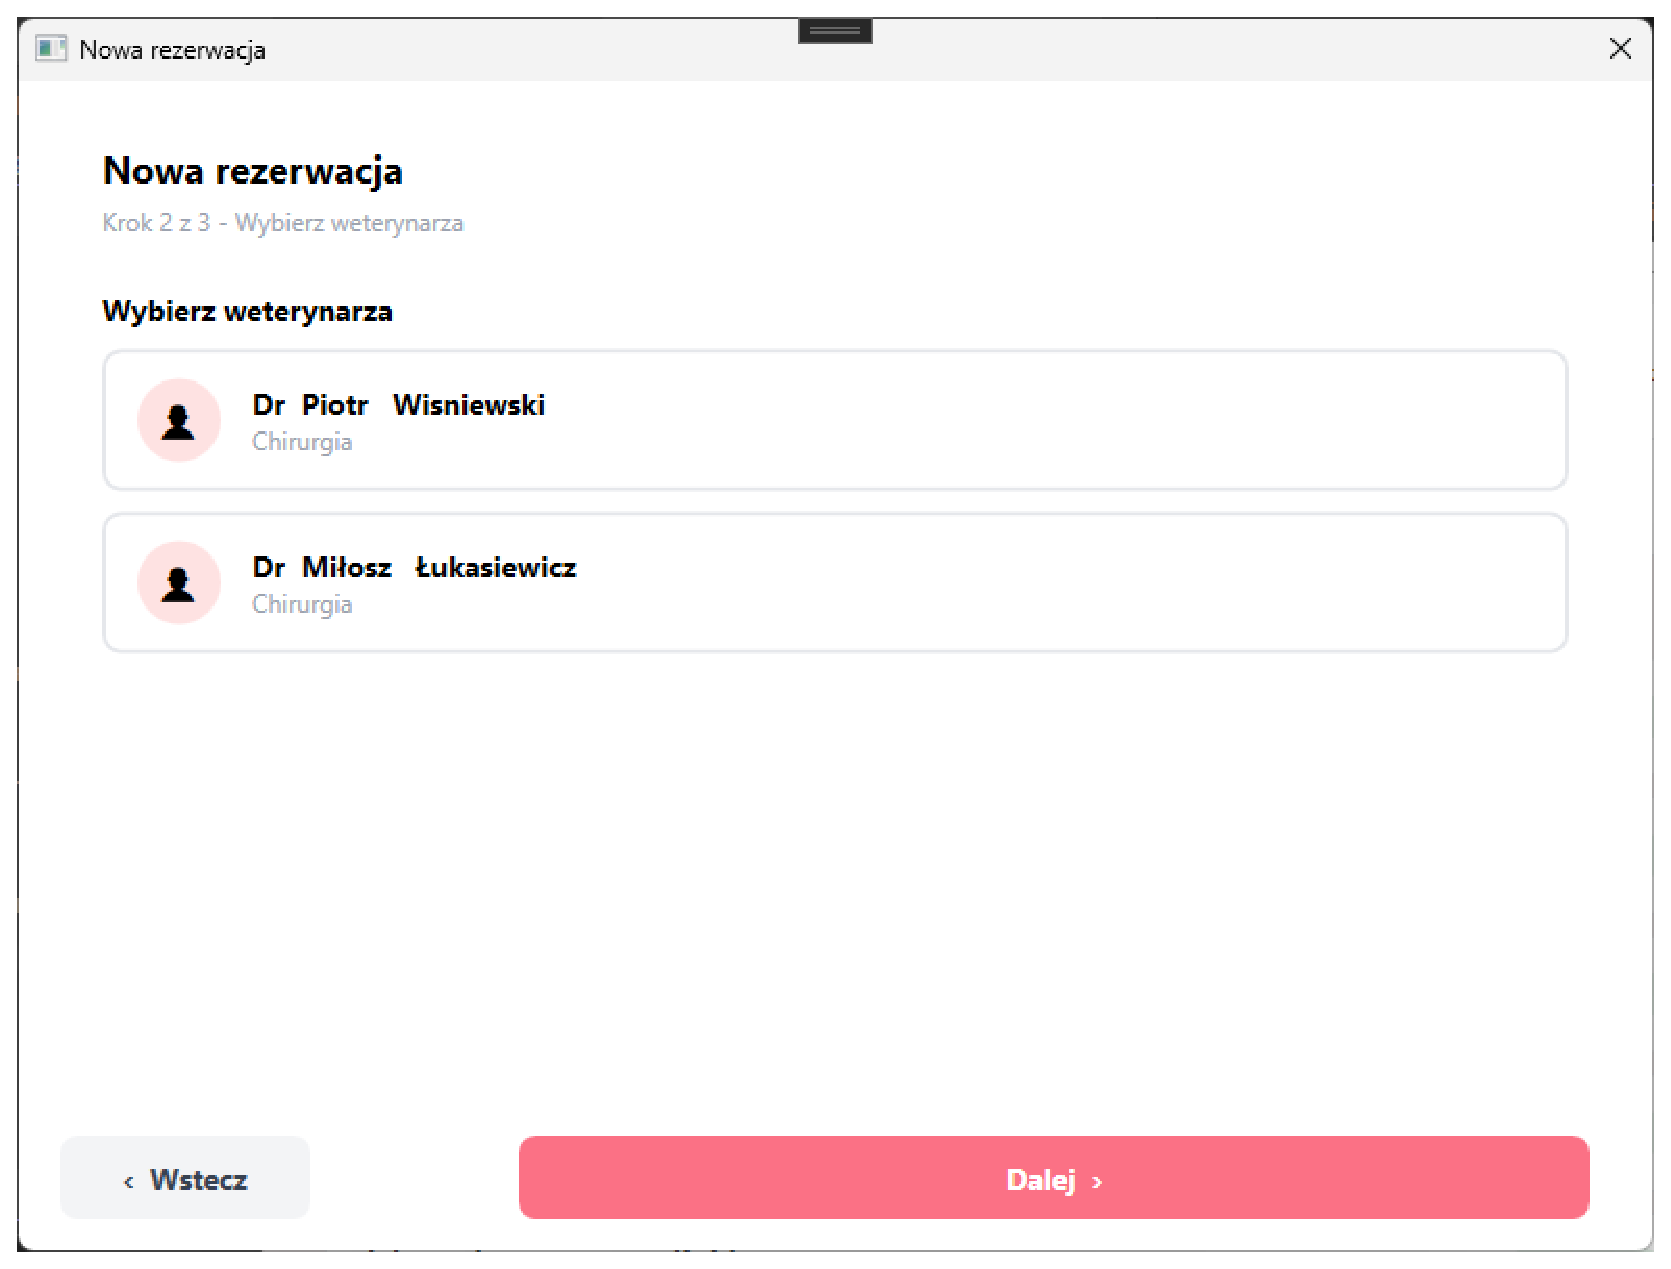
\includegraphics[width=0.9\linewidth]{figures/Uzytkownik/fig_030.eps}
\caption{Krok 2 - widok wyboru weterynarza.\label{fig30}}
\end{figure}

W przypadku gdy użytkownik nie wybierze weterynarza przed kliknięciem przycisku Dalej, aplikacja wyświetla komunikat błędu.

\begin{figure}[H]
\centering
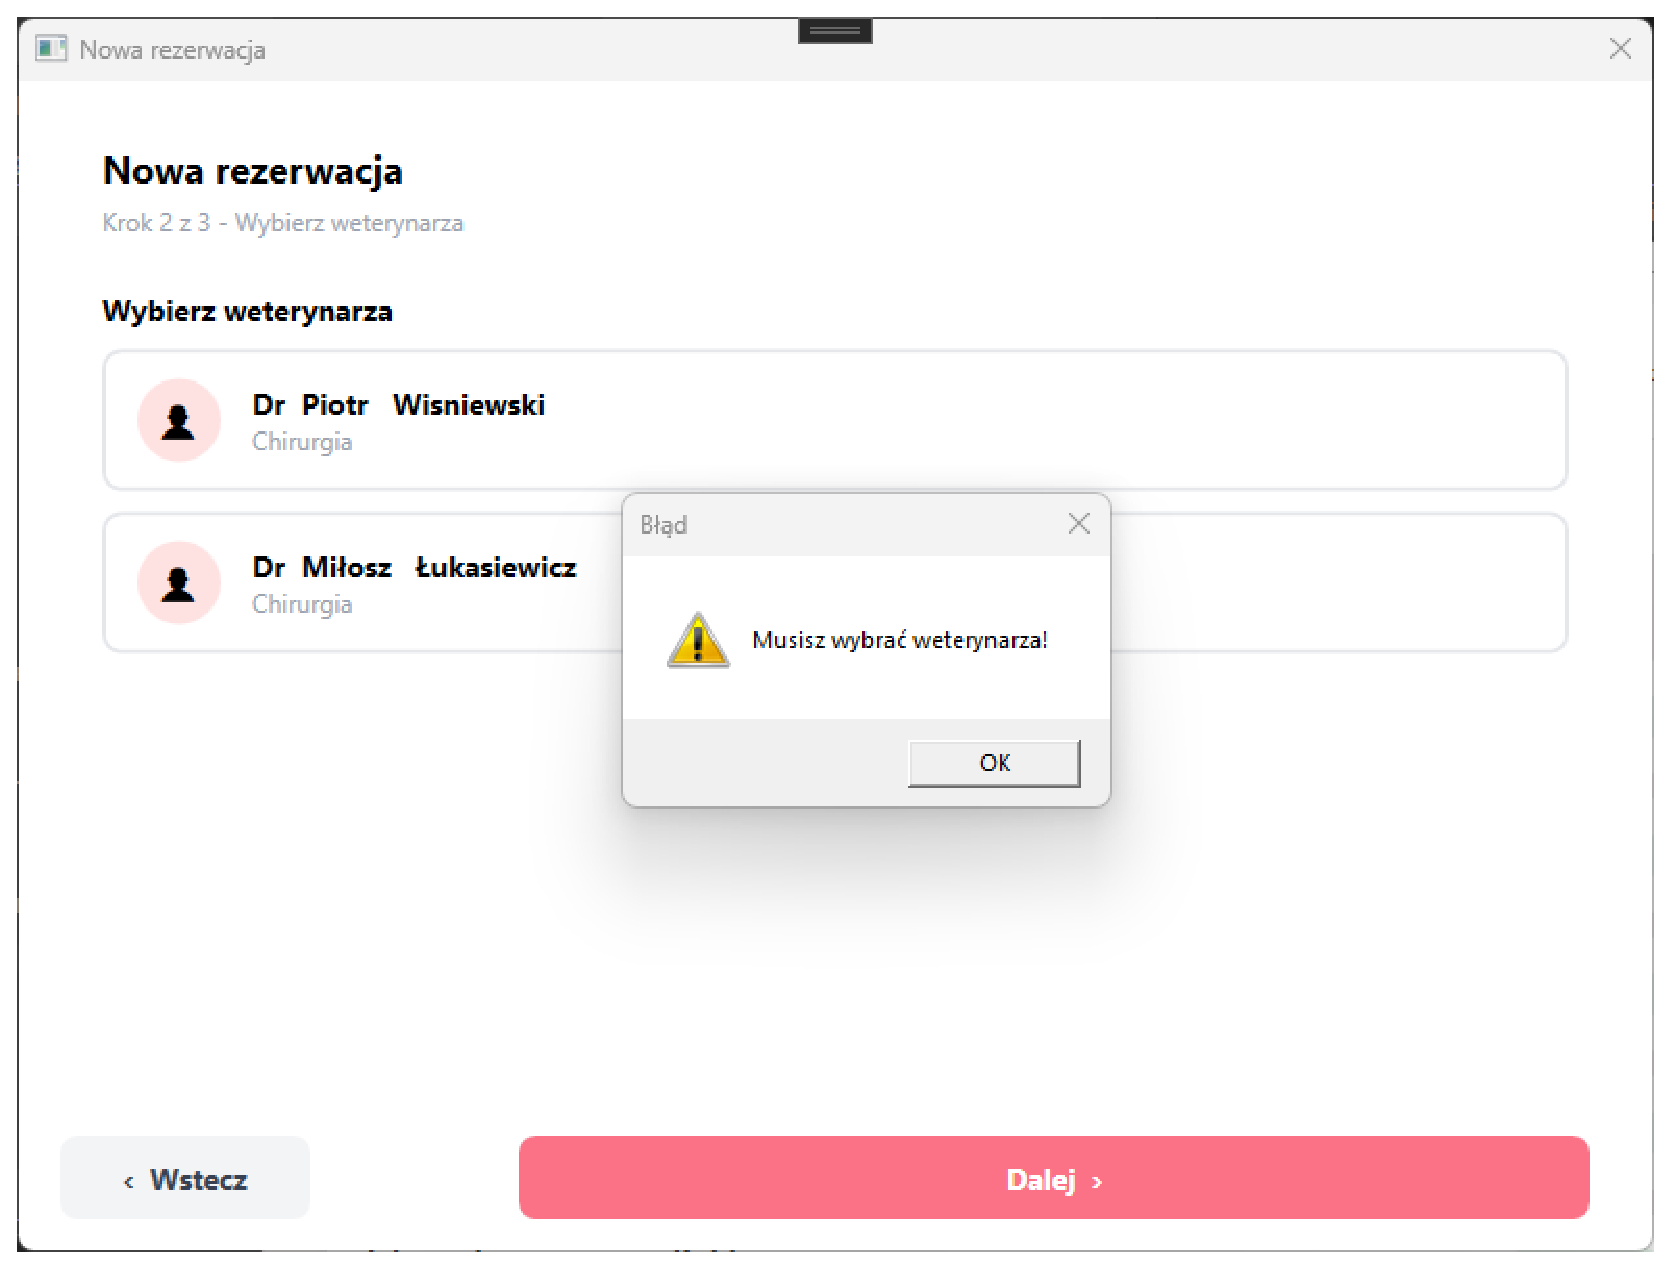
\includegraphics[width=0.9\linewidth]{figures/Uzytkownik/fig_031.eps}
\caption{Komunikat błędu przy braku wybranego weterynarza.\label{fig31}}
\end{figure}

W trzecim kroku użytkownik wybiera termin wizyty z kalendarza dostępności wybranego weterynarza. 
Kalendarz prezentuje tygodniowy widok z podziałem na godziny. Sloty oznaczone kolorem zielonym 
są wolne i możliwe do zarezerwowania, czerwonym zajęte, natomiast szare oznaczają terminy poza 
godzinami pracy weterynarza lub terminy w których zabieg nie zmieści się przed końcem pracy.

\begin{figure}[H]
\centering
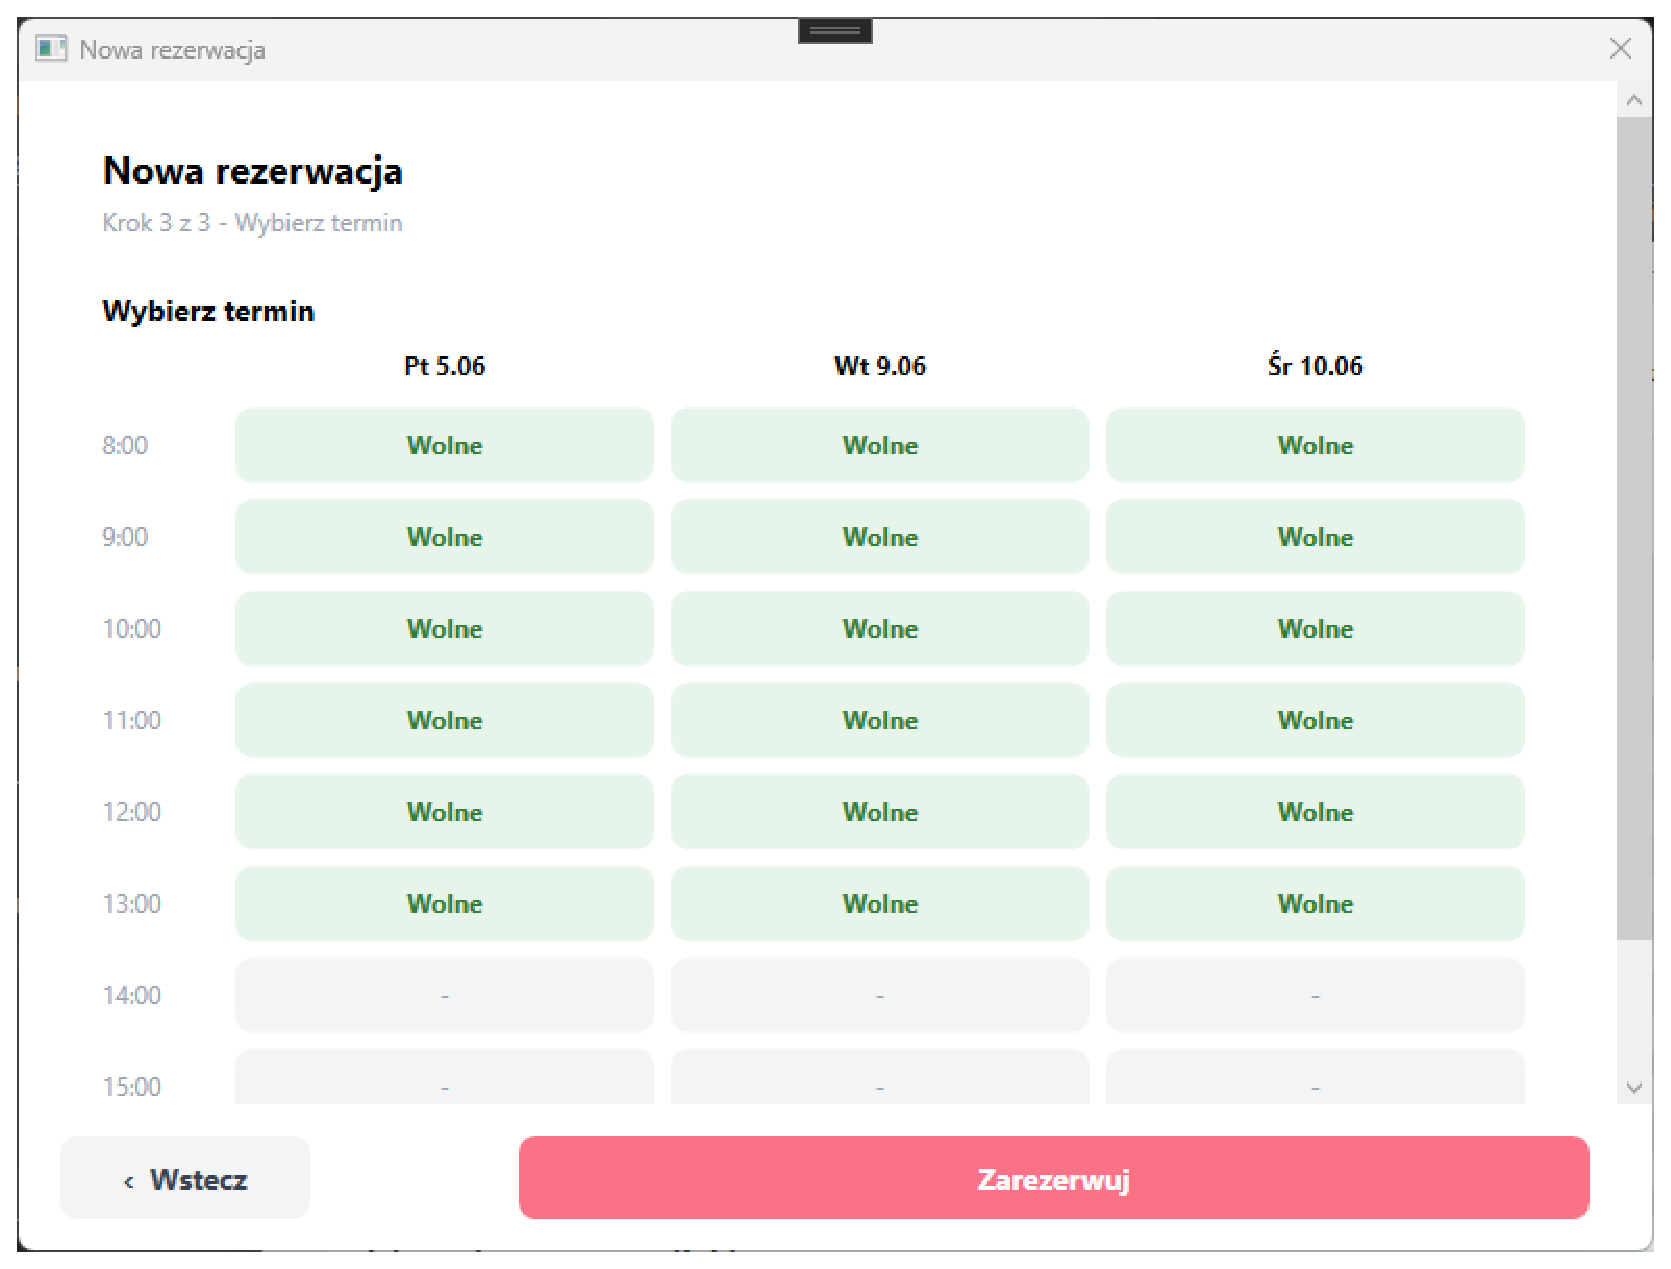
\includegraphics[width=0.9\linewidth]{figures/Uzytkownik/fig_032.eps}
\caption{Krok 3 - widok kalendarza dostępności weterynarza.\label{fig32}}
\end{figure}

W przypadku gdy użytkownik nie wybierze terminu przed kliknięciem przycisku Zarezerwuj, aplikacja wyświetla komunikat błędu.

\begin{figure}[H]
\centering
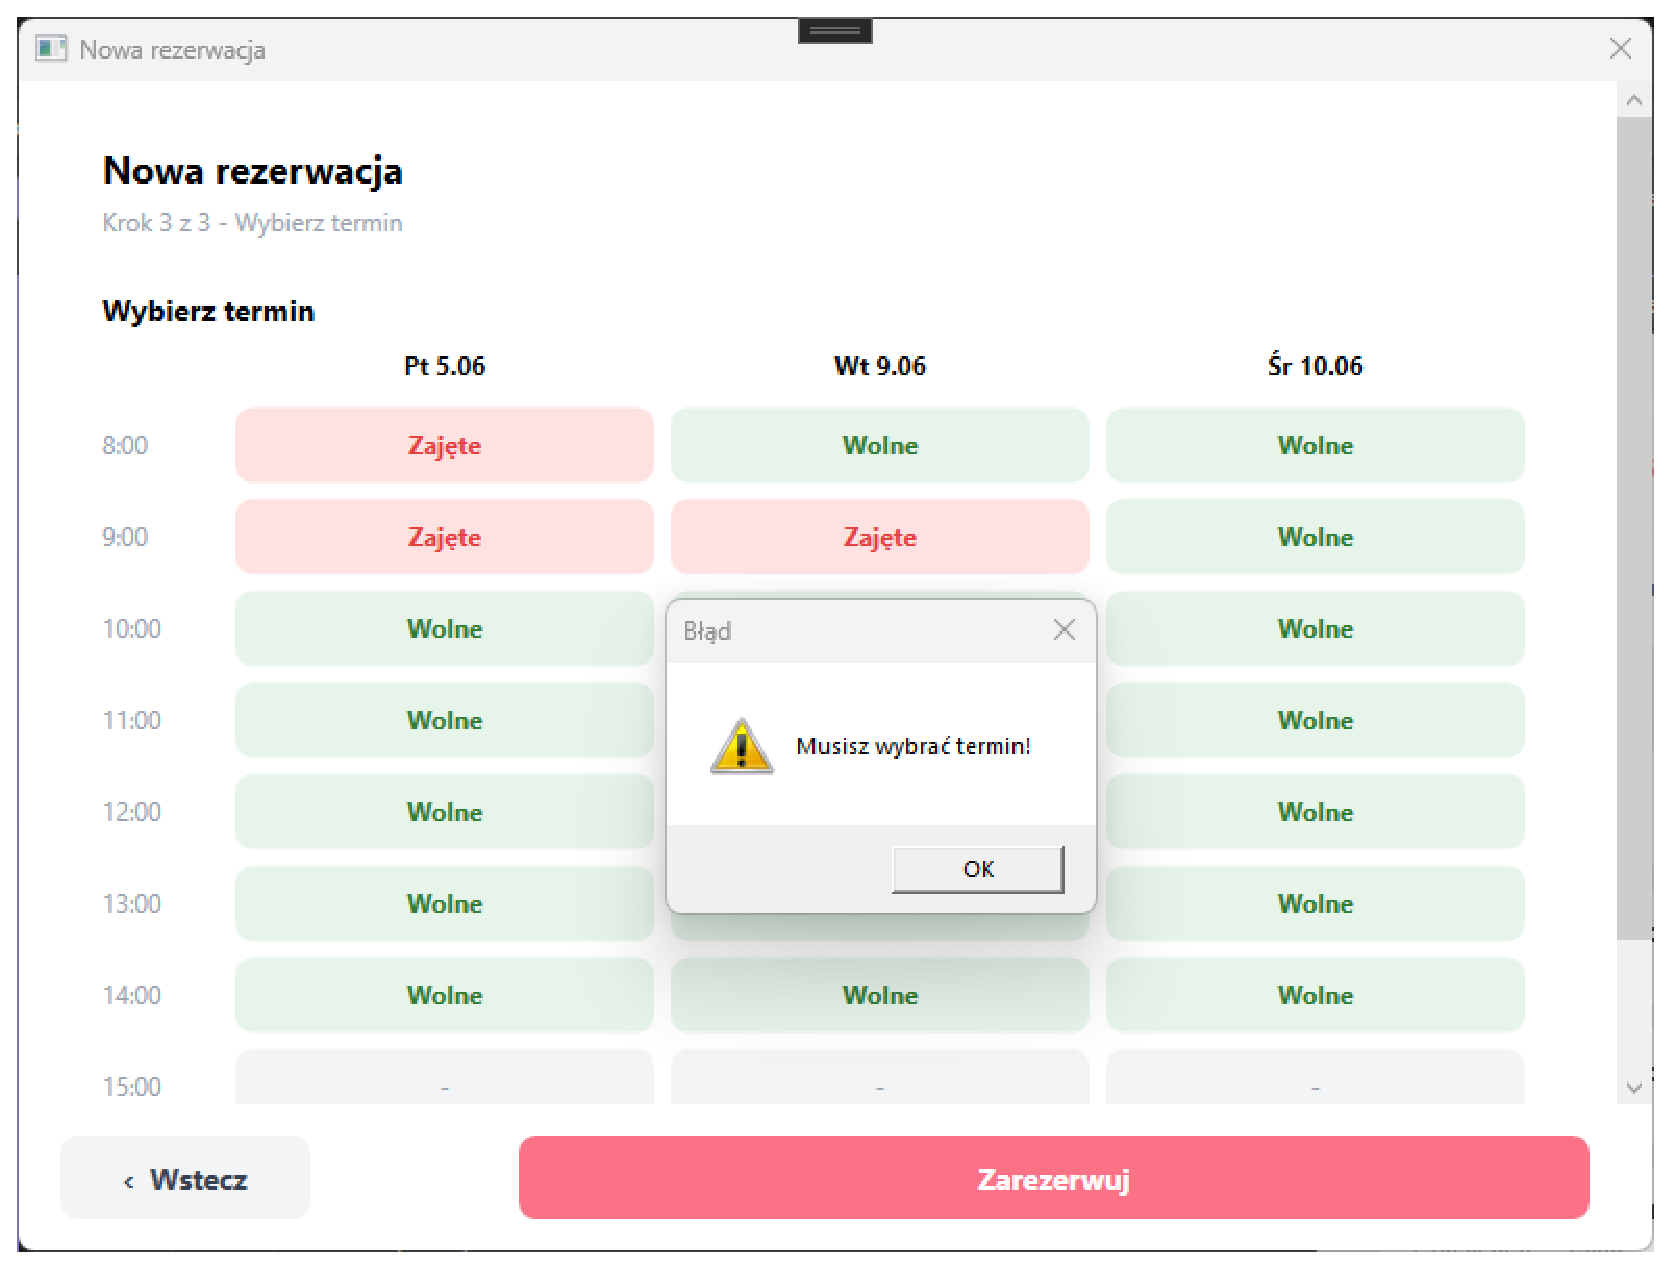
\includegraphics[width=0.9\linewidth]{figures/Uzytkownik/fig_033.eps}
\caption{Komunikat błędu przy braku wybranego terminu.\label{fig33}}
\end{figure}

Po wybraniu wolnego terminu i kliknięciu przycisku Zarezerwuj rezerwacja zostaje zapisana w bazie danych, a z 
konta użytkownika pobierana jest kwota odpowiadająca cenie zabiegu. Aplikacja wyświetla komunikat potwierdzający 
pomyślne zapisanie rezerwacji wraz z informacją o pobranej kwocie oraz pozostałym saldzie.

\begin{figure}[H]
\centering
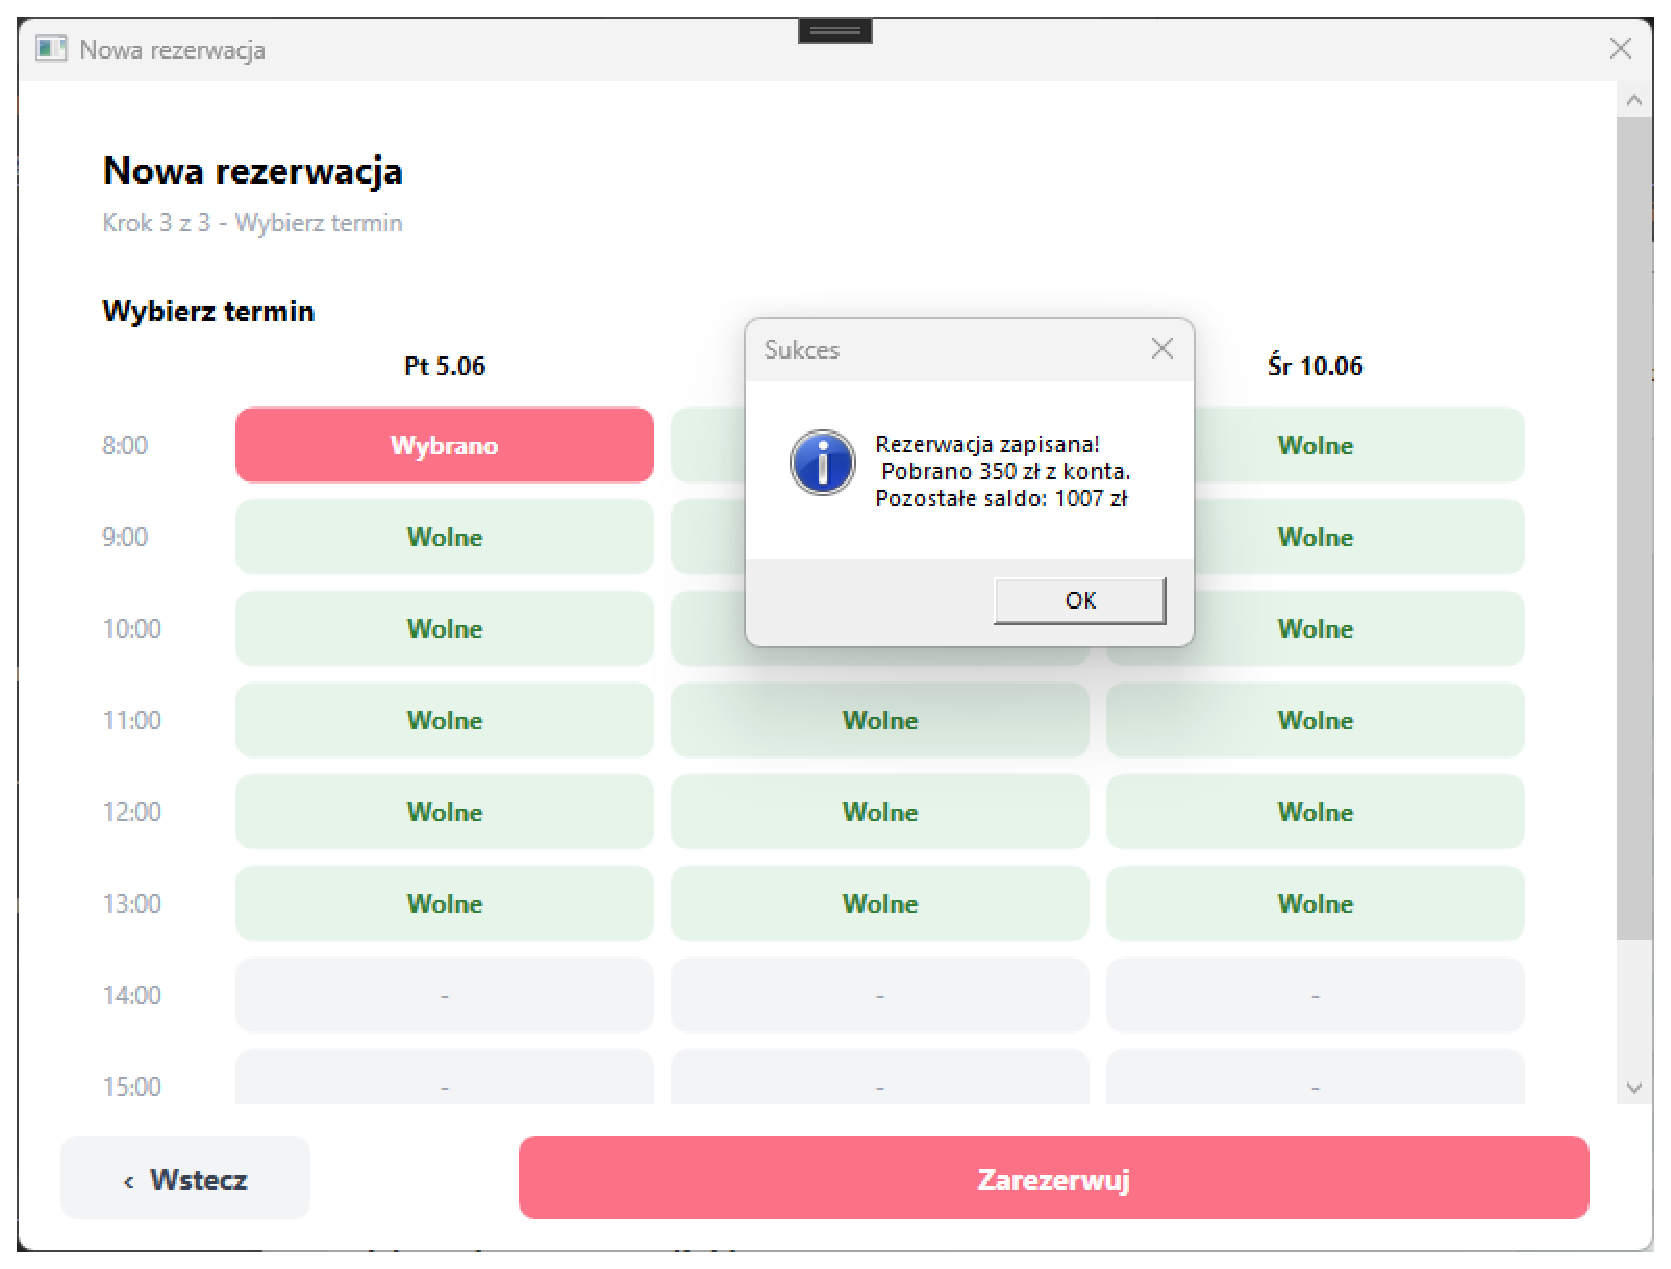
\includegraphics[width=0.9\linewidth]{figures/Uzytkownik/fig_034.eps}
\caption{Komunikat potwierdzający pomyślne zapisanie rezerwacji.\label{fig34}}
\end{figure}

\textbf{Zakładka "Dodaj środki"}

Zakładka "Dodaj środki" umożliwia użytkownikowi doładowanie salda swojego konta. Formularz zawiera jedno pole tekstowe 
do wprowadzenia kwoty wpłaty oraz przycisk Wpłać. Aktualne saldo konta wyświetlane jest na bieżąco w górnym pasku aplikacji.

\begin{figure}[H]
\centering
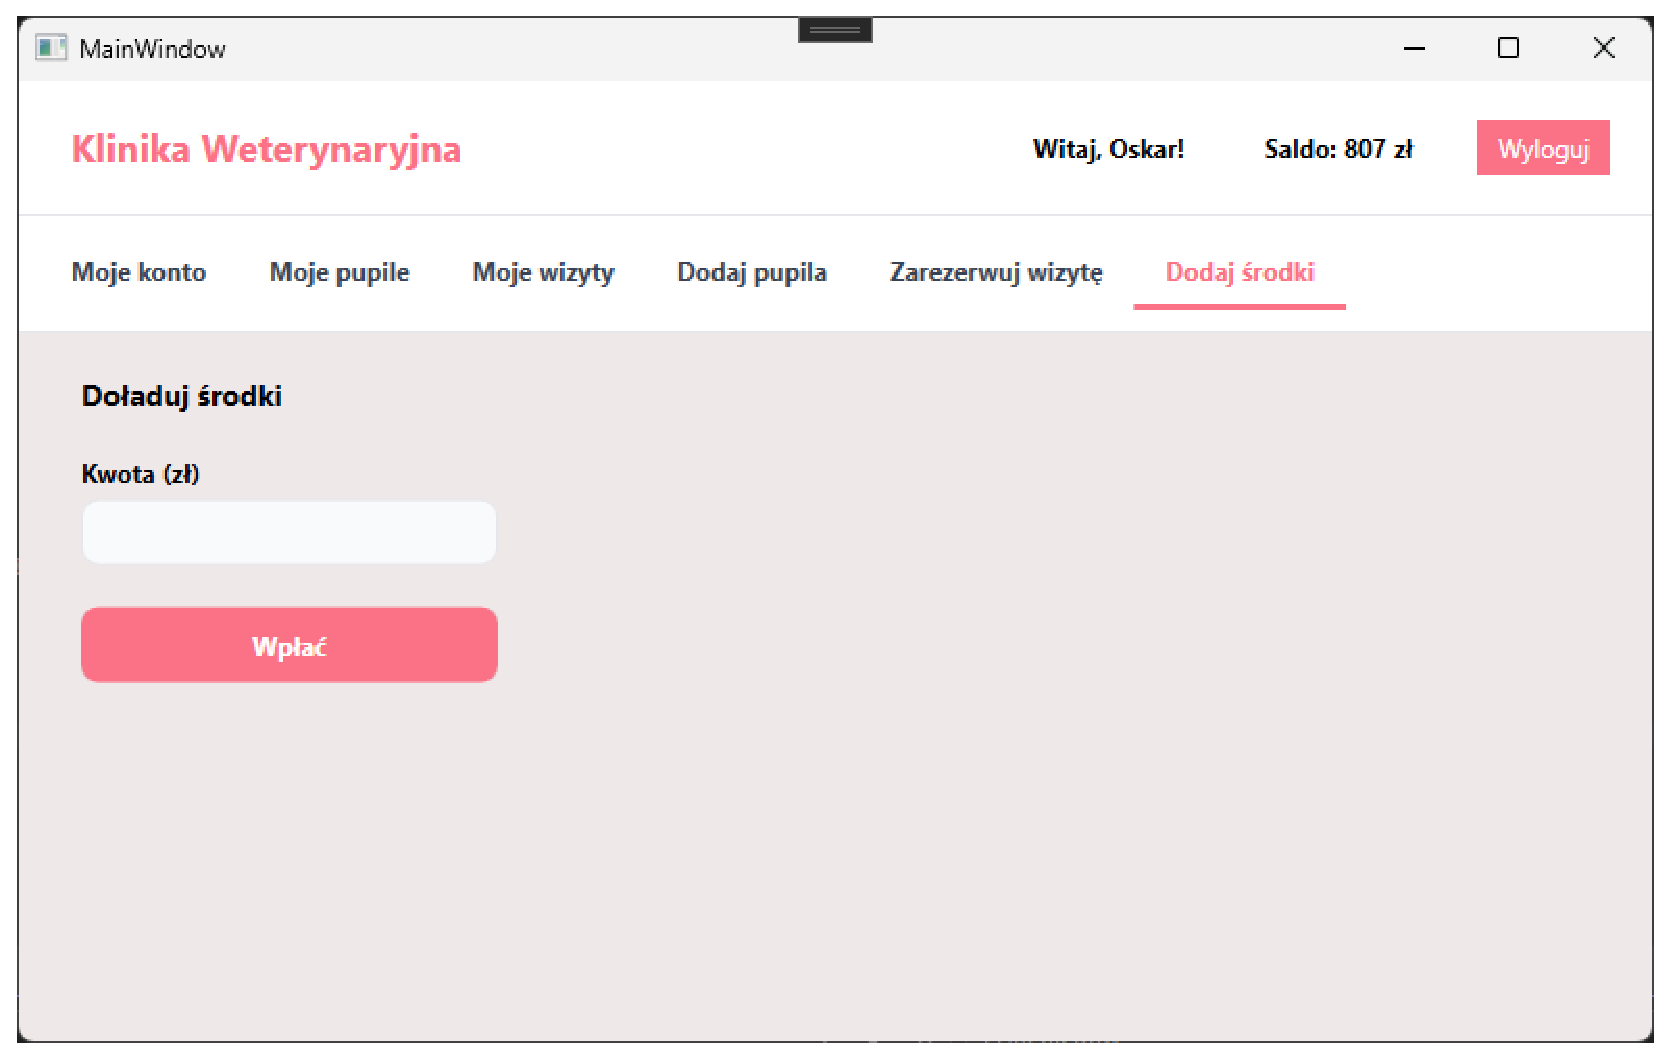
\includegraphics[width=0.9\linewidth]{figures/Uzytkownik/fig_035.eps}
\caption{Widok zakładki Dodaj środki.\label{fig35}}
\end{figure}

W przypadku gdy użytkownik nie wprowadzi żadnej kwoty i kliknie przycisk Wpłać, aplikacja wyświetla komunikat 
błędu informujący o konieczności podania prawidłowej kwoty.

\begin{figure}[H]
\centering
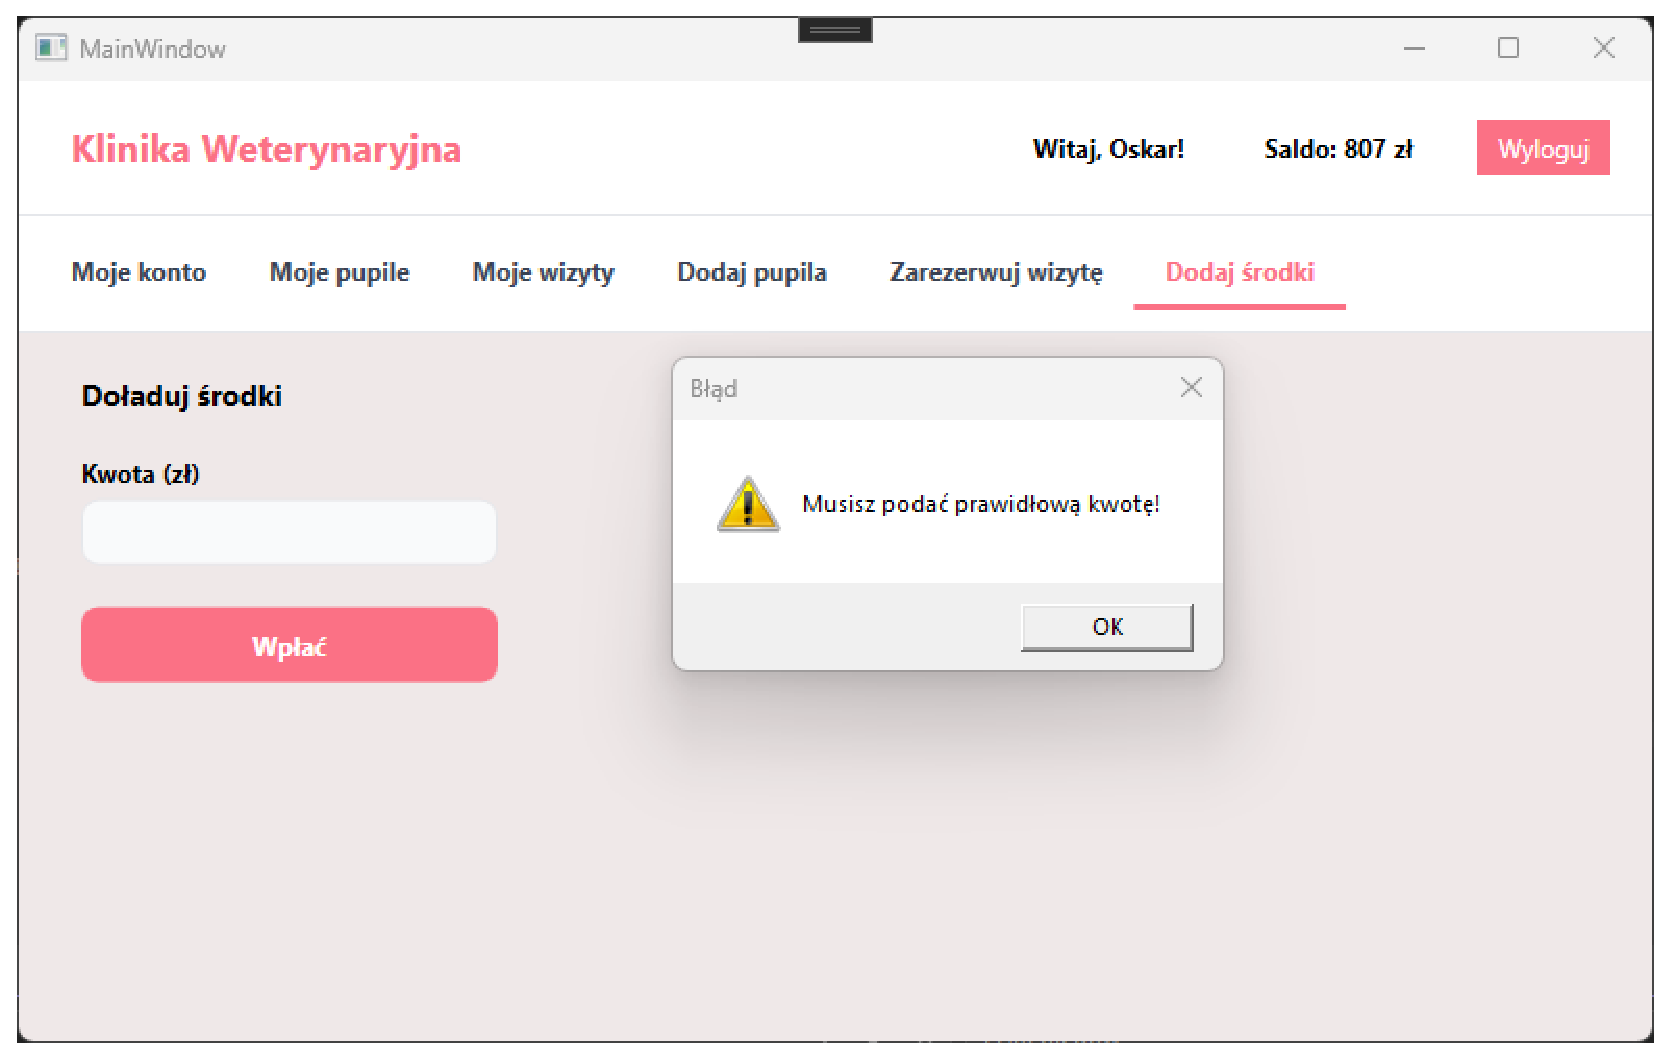
\includegraphics[width=0.9\linewidth]{figures/Uzytkownik/fig_036.eps}
\caption{Komunikat błędu przy pustym polu kwoty.\label{fig36}}
\end{figure}

Aplikacja waliduje również podaną kwotę - nie może ona być liczbą ujemną ani równą zero. 
W przypadku podania nieprawidłowej wartości wyświetlany jest komunikat błędu.

\begin{figure}[H]
\centering
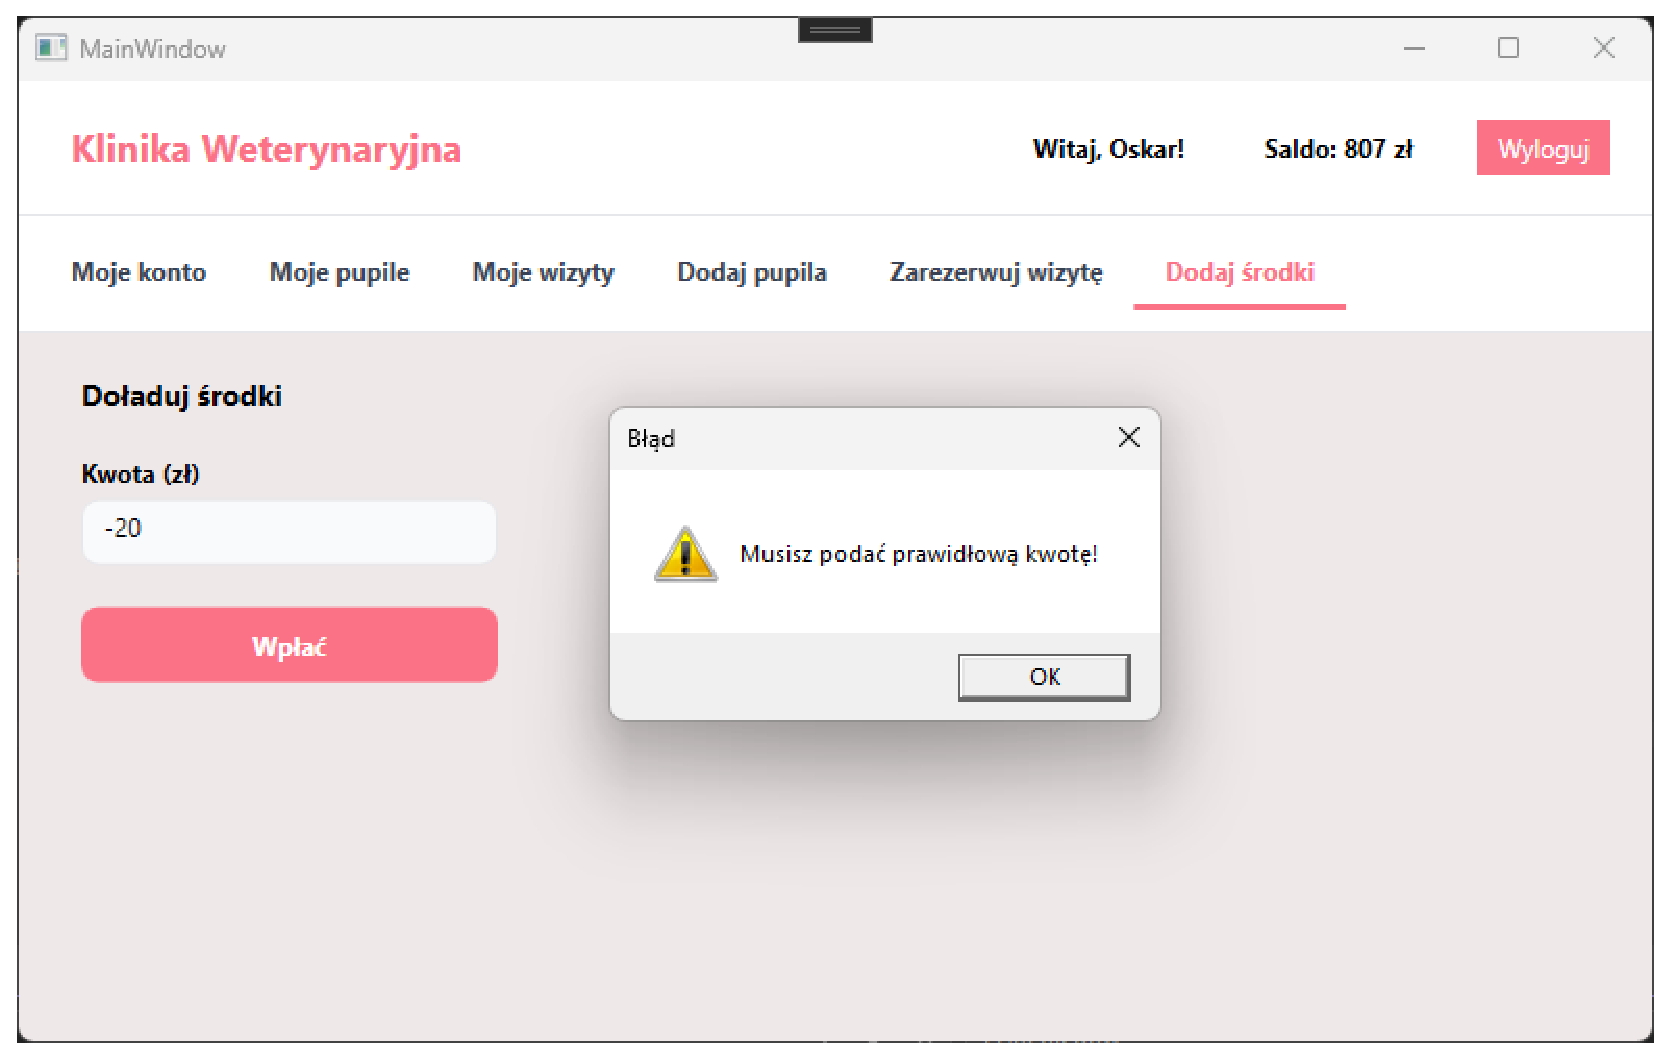
\includegraphics[width=0.9\linewidth]{figures/Uzytkownik/fig_037.eps}
\caption{Komunikat błędu przy podaniu nieprawidłowej kwoty.\label{fig37}}
\end{figure}

Po wprowadzeniu prawidłowej kwoty i kliknięciu przycisku Wpłać aplikacja wyświetla okno dialogowe z prośbą o potwierdzenie 
operacji, informując o kwocie która zostanie dodana do salda.

\begin{figure}[H]
\centering
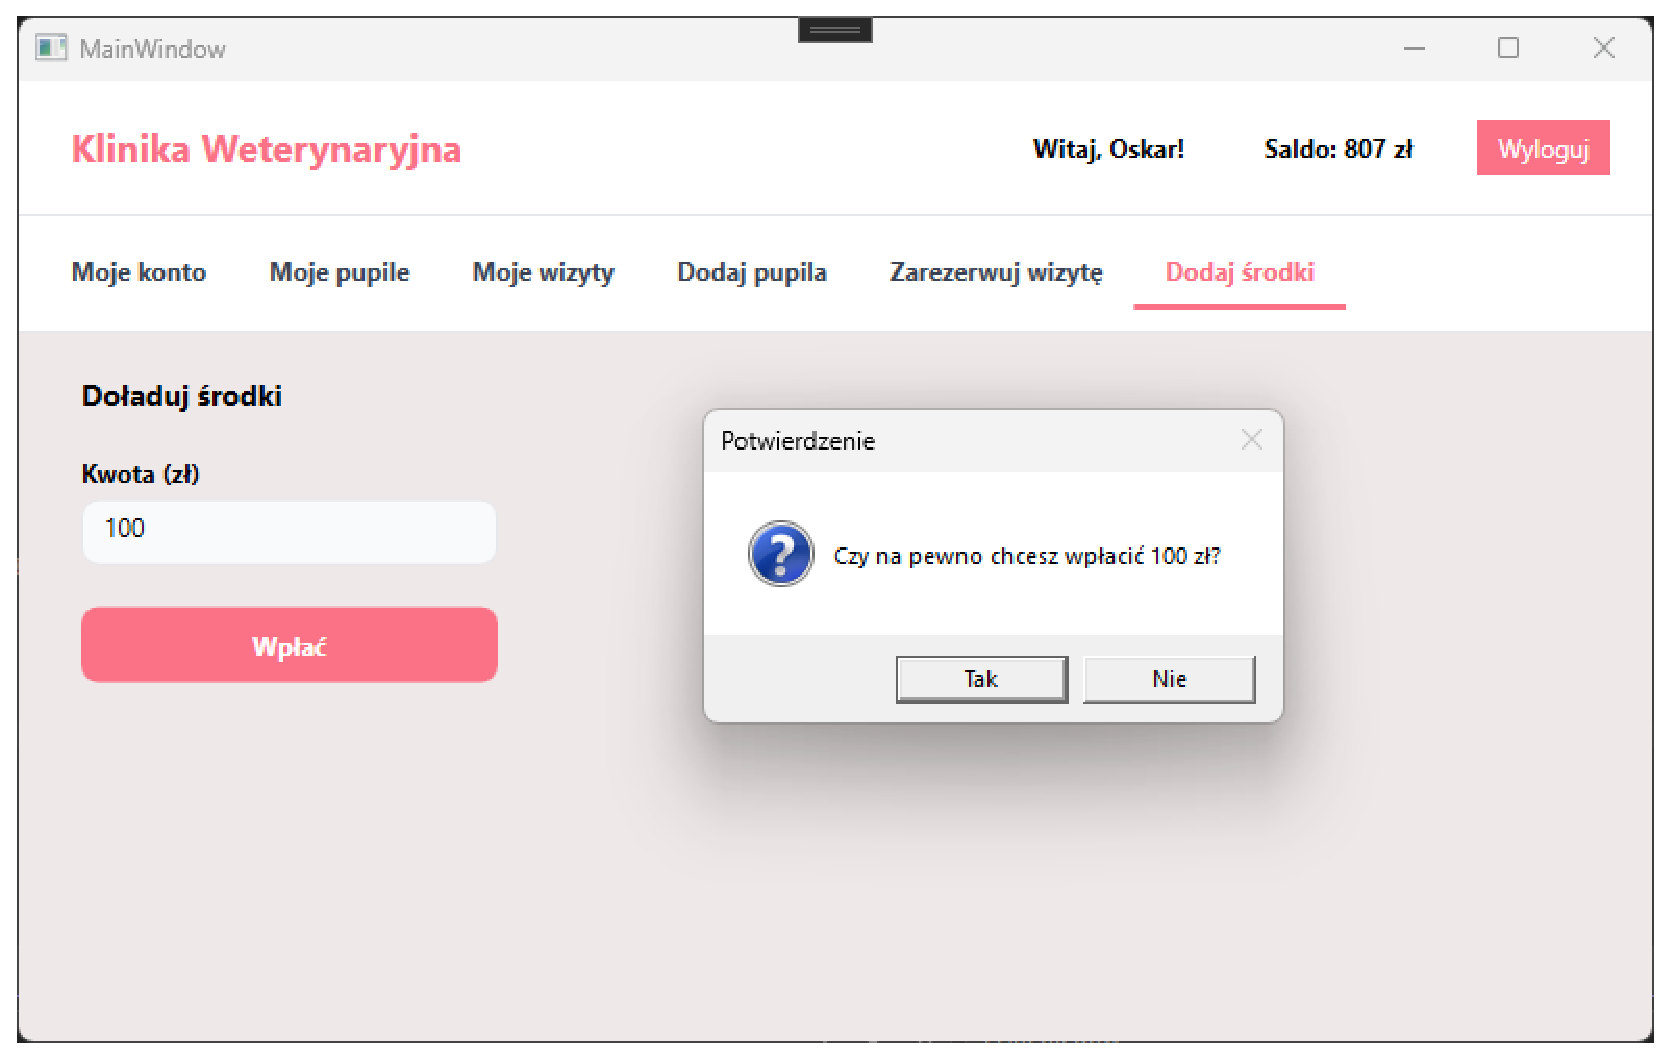
\includegraphics[width=0.9\linewidth]{figures/Uzytkownik/fig_038.eps}
\caption{Okno potwierdzenia wpłaty środków.\label{fig38}}
\end{figure}

Po zatwierdzeniu operacji saldo konta użytkownika zostaje zwiększone o podaną kwotę, zarówno w bazie 
danych jak i w interfejsie aplikacji. Aplikacja wyświetla komunikat potwierdzający pomyślne wykonanie 
wpłaty, a pole tekstowe zostaje wyczyszczone.

\begin{figure}[H]
\centering
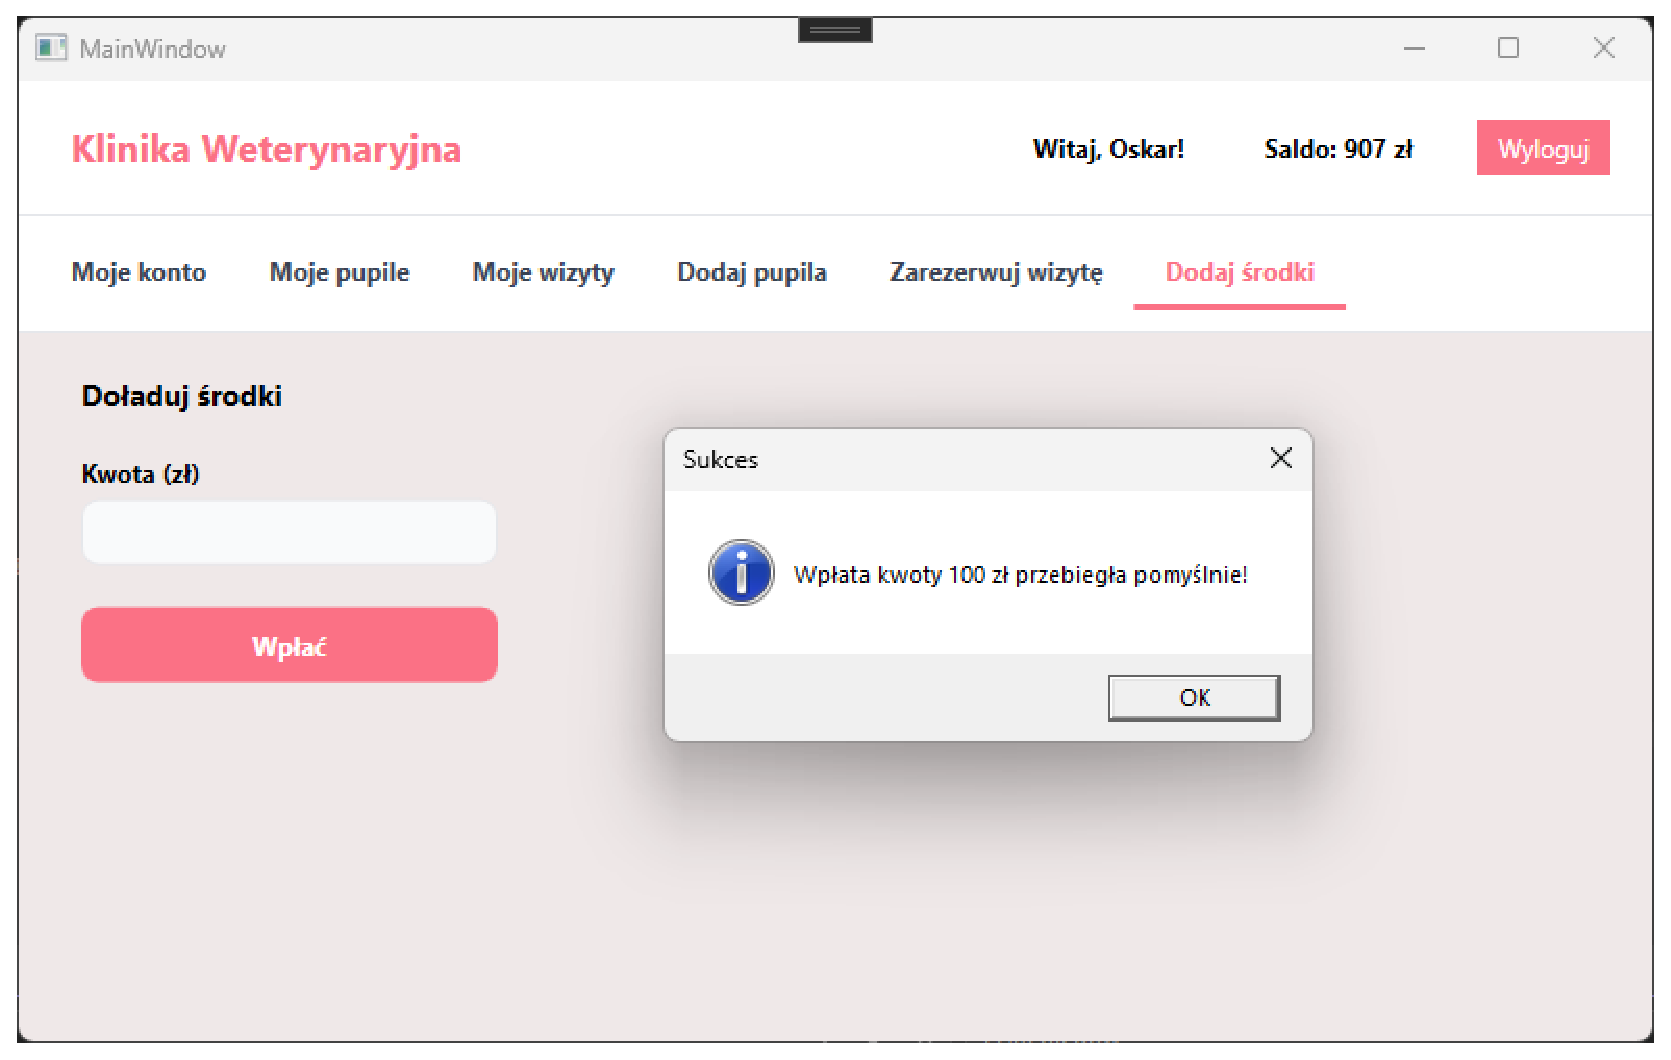
\includegraphics[width=0.9\linewidth]{figures/Uzytkownik/fig_039.eps}
\caption{Komunikat potwierdzający pomyślną wpłatę środków.\label{fig39}}
\end{figure}

\section{Panel administratora}

\textbf{Zakładka "Weterynarze"}

Zakładka "Weterynarze" wyświetla listę wszystkich weterynarzy zarejestrowanych w systemie. Dla każdego weterynarza 
prezentowane są informacje takie jak imię, nazwisko, specjalizacja, adres e-mail oraz numer telefonu. 
Przy każdym weterynarzu dostępne są dwa przyciski akcji: + umożliwiający zarządzanie zabiegami przypisanymi do weterynarza oraz X umożliwiający 
usunięcie weterynarza z systemu. W prawym górnym rogu zakładki znajduje się przycisk (+ Dodaj weterynarza).

\begin{figure}[H]
\centering
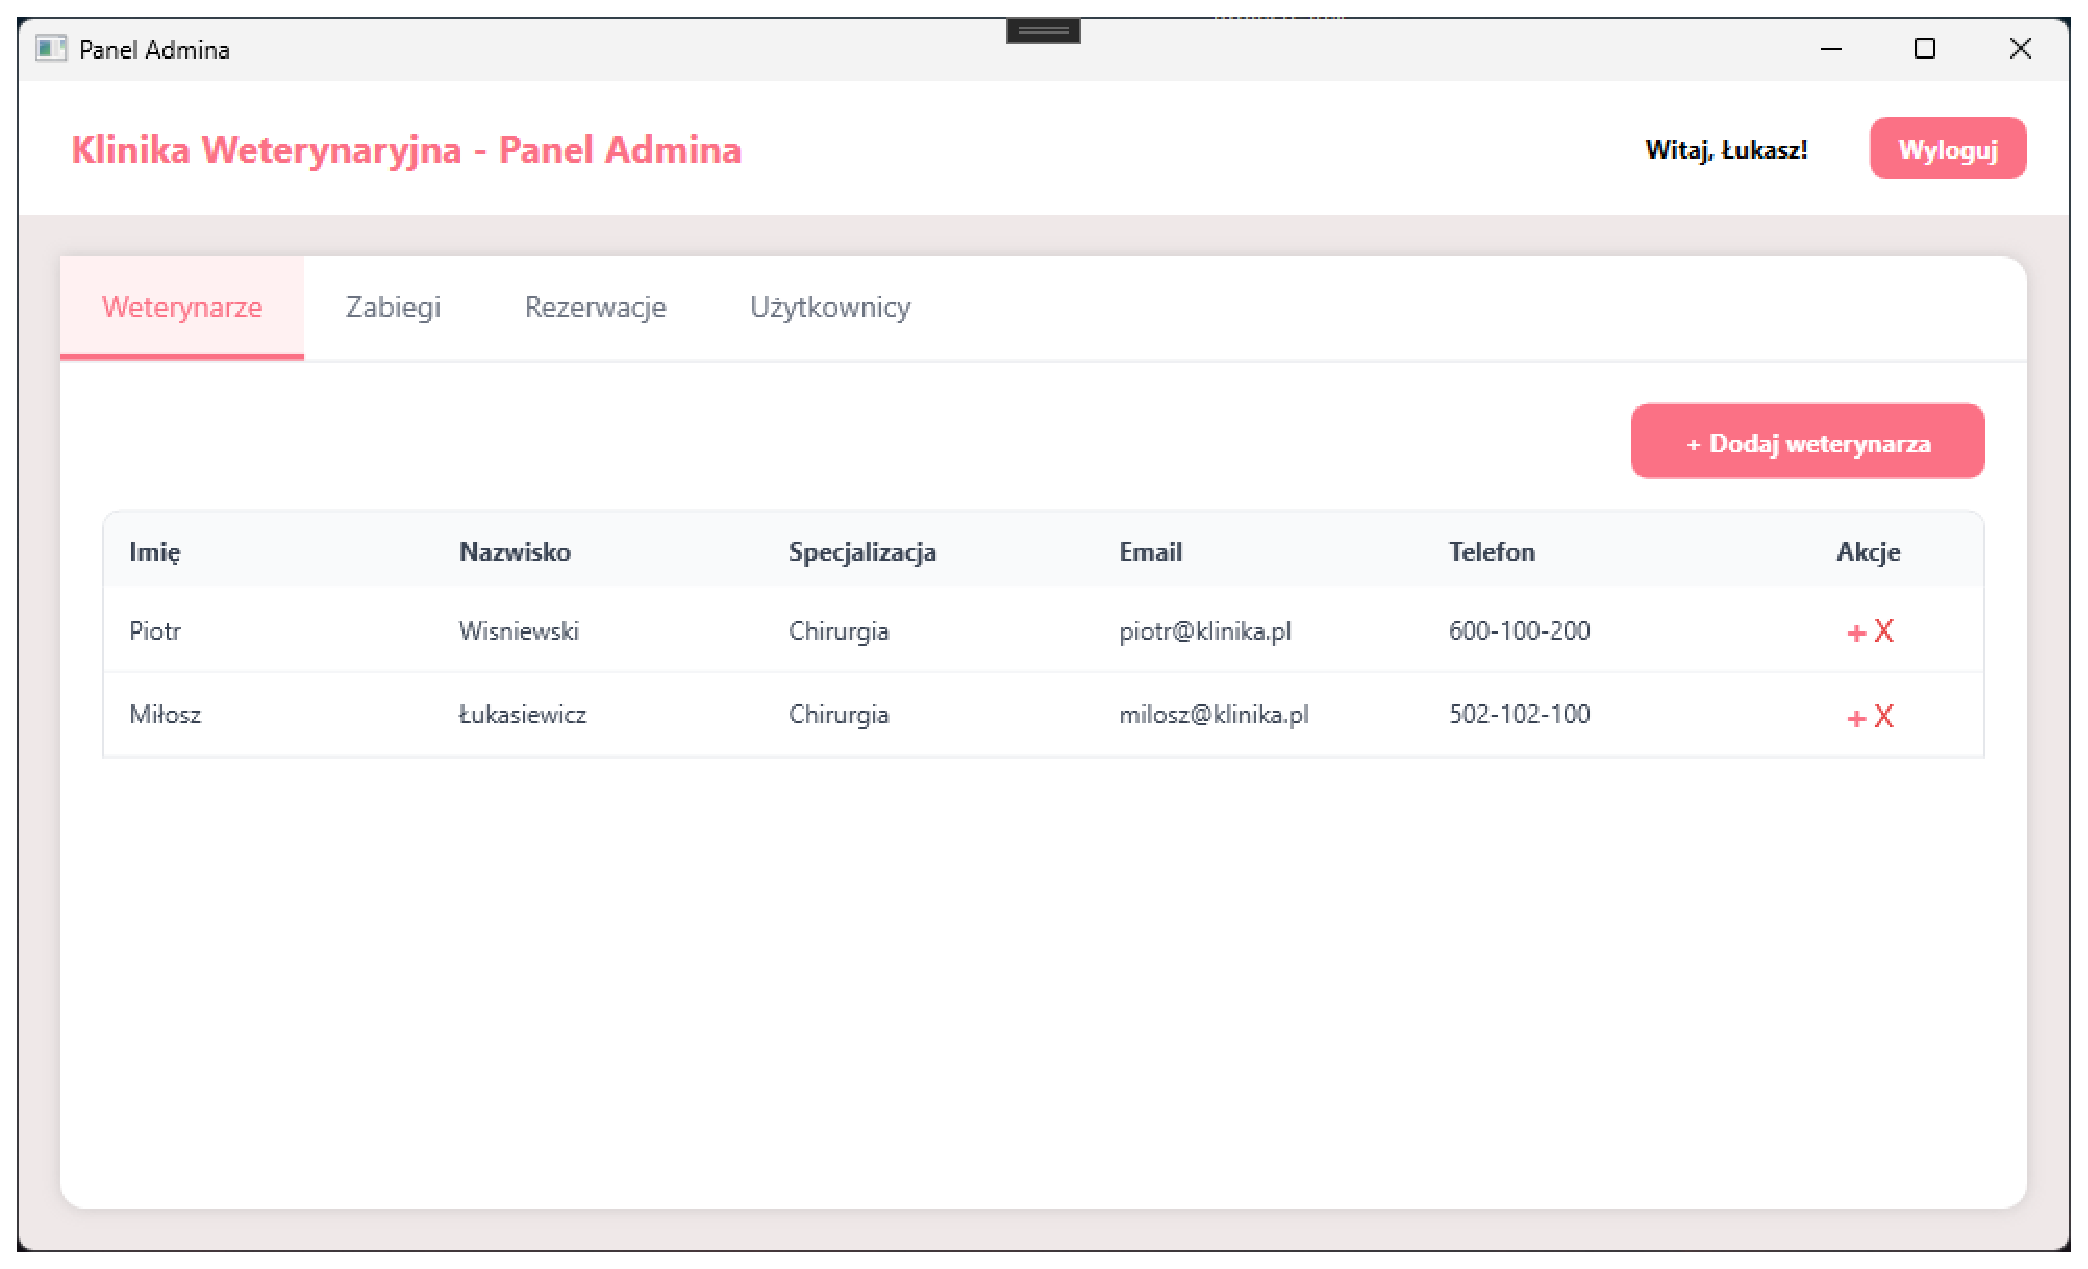
\includegraphics[width=0.9\linewidth]{figures/Admin/fig_040.eps}
\caption{Widok zakładki Weterynarze w panelu administratora.\label{fig40}}
\end{figure}

Po kliknięciu przycisku (+ Dodaj weterynarza) otwierane jest okno formularza. 
Formularz zawiera pola: imię, nazwisko, specjalizacja, email, telefon, hasło oraz sekcję Godziny pracy z polami 
Od i Do dla każdego dnia tygodnia od poniedziałku do piątku. Domyślne godziny pracy ustawione są na 08:00-15:00. Pozostawienie pól 
pustych dla danego dnia oznacza, że weterynarz nie pracuje w tym dniu.

\begin{figure}[H]
\centering
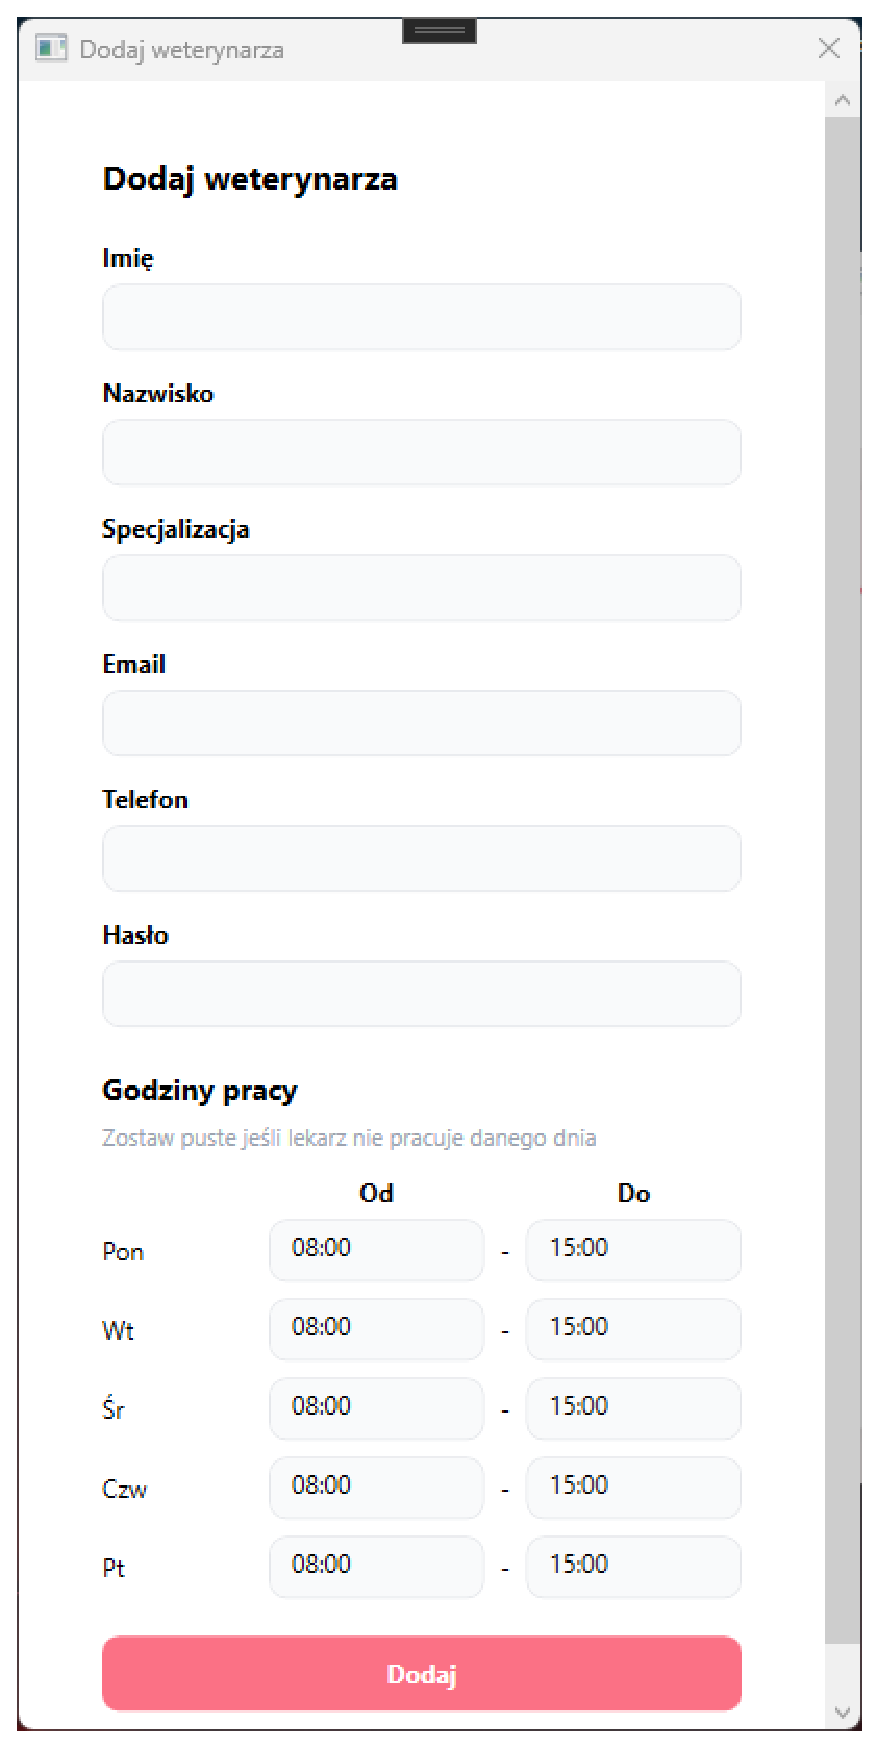
\includegraphics[width=0.6\linewidth]{figures/Admin/fig_041.eps}
\caption{Okno formularza dodawania weterynarza.\label{fig41}}
\end{figure}

W przypadku gdy administrator nie wypełni wymaganych pól (imię, nazwisko, email, hasło) aplikacja wyświetla komunikat błędu.

\begin{figure}[H]
\centering
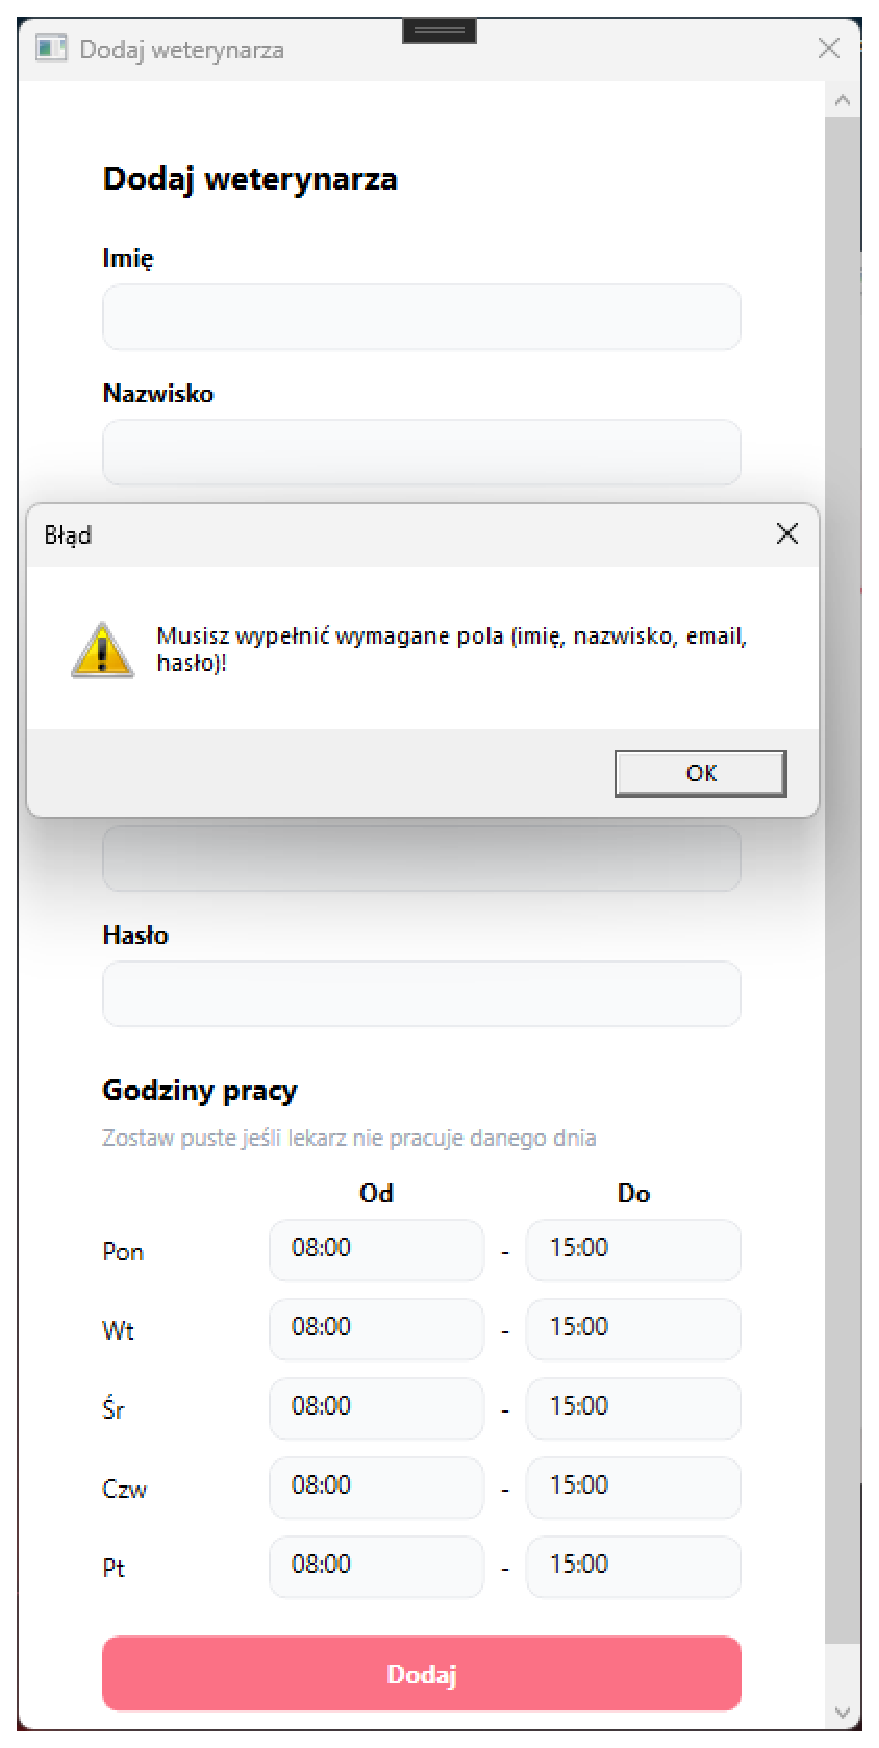
\includegraphics[width=0.6\linewidth]{figures/Admin/fig_042.eps}
\caption{Komunikat błędu przy niewypełnionych wymaganych polach.\label{fig42}}
\end{figure}

Po kliknięciu przycisku + przy wybranym weterynarzu otwierane jest okno zarządzania zabiegami. 
Wyświetlana jest lista wszystkich dostępnych zabiegów z checkboxami, zaznaczone zabiegi oznaczają te, 
które dany weterynarz aktualnie wykonuje. Administrator może dowolnie zaznaczać i odznaczać zabiegi, a następnie zapisać zmiany przyciskiem Zapisz.

\begin{figure}[H]
\centering
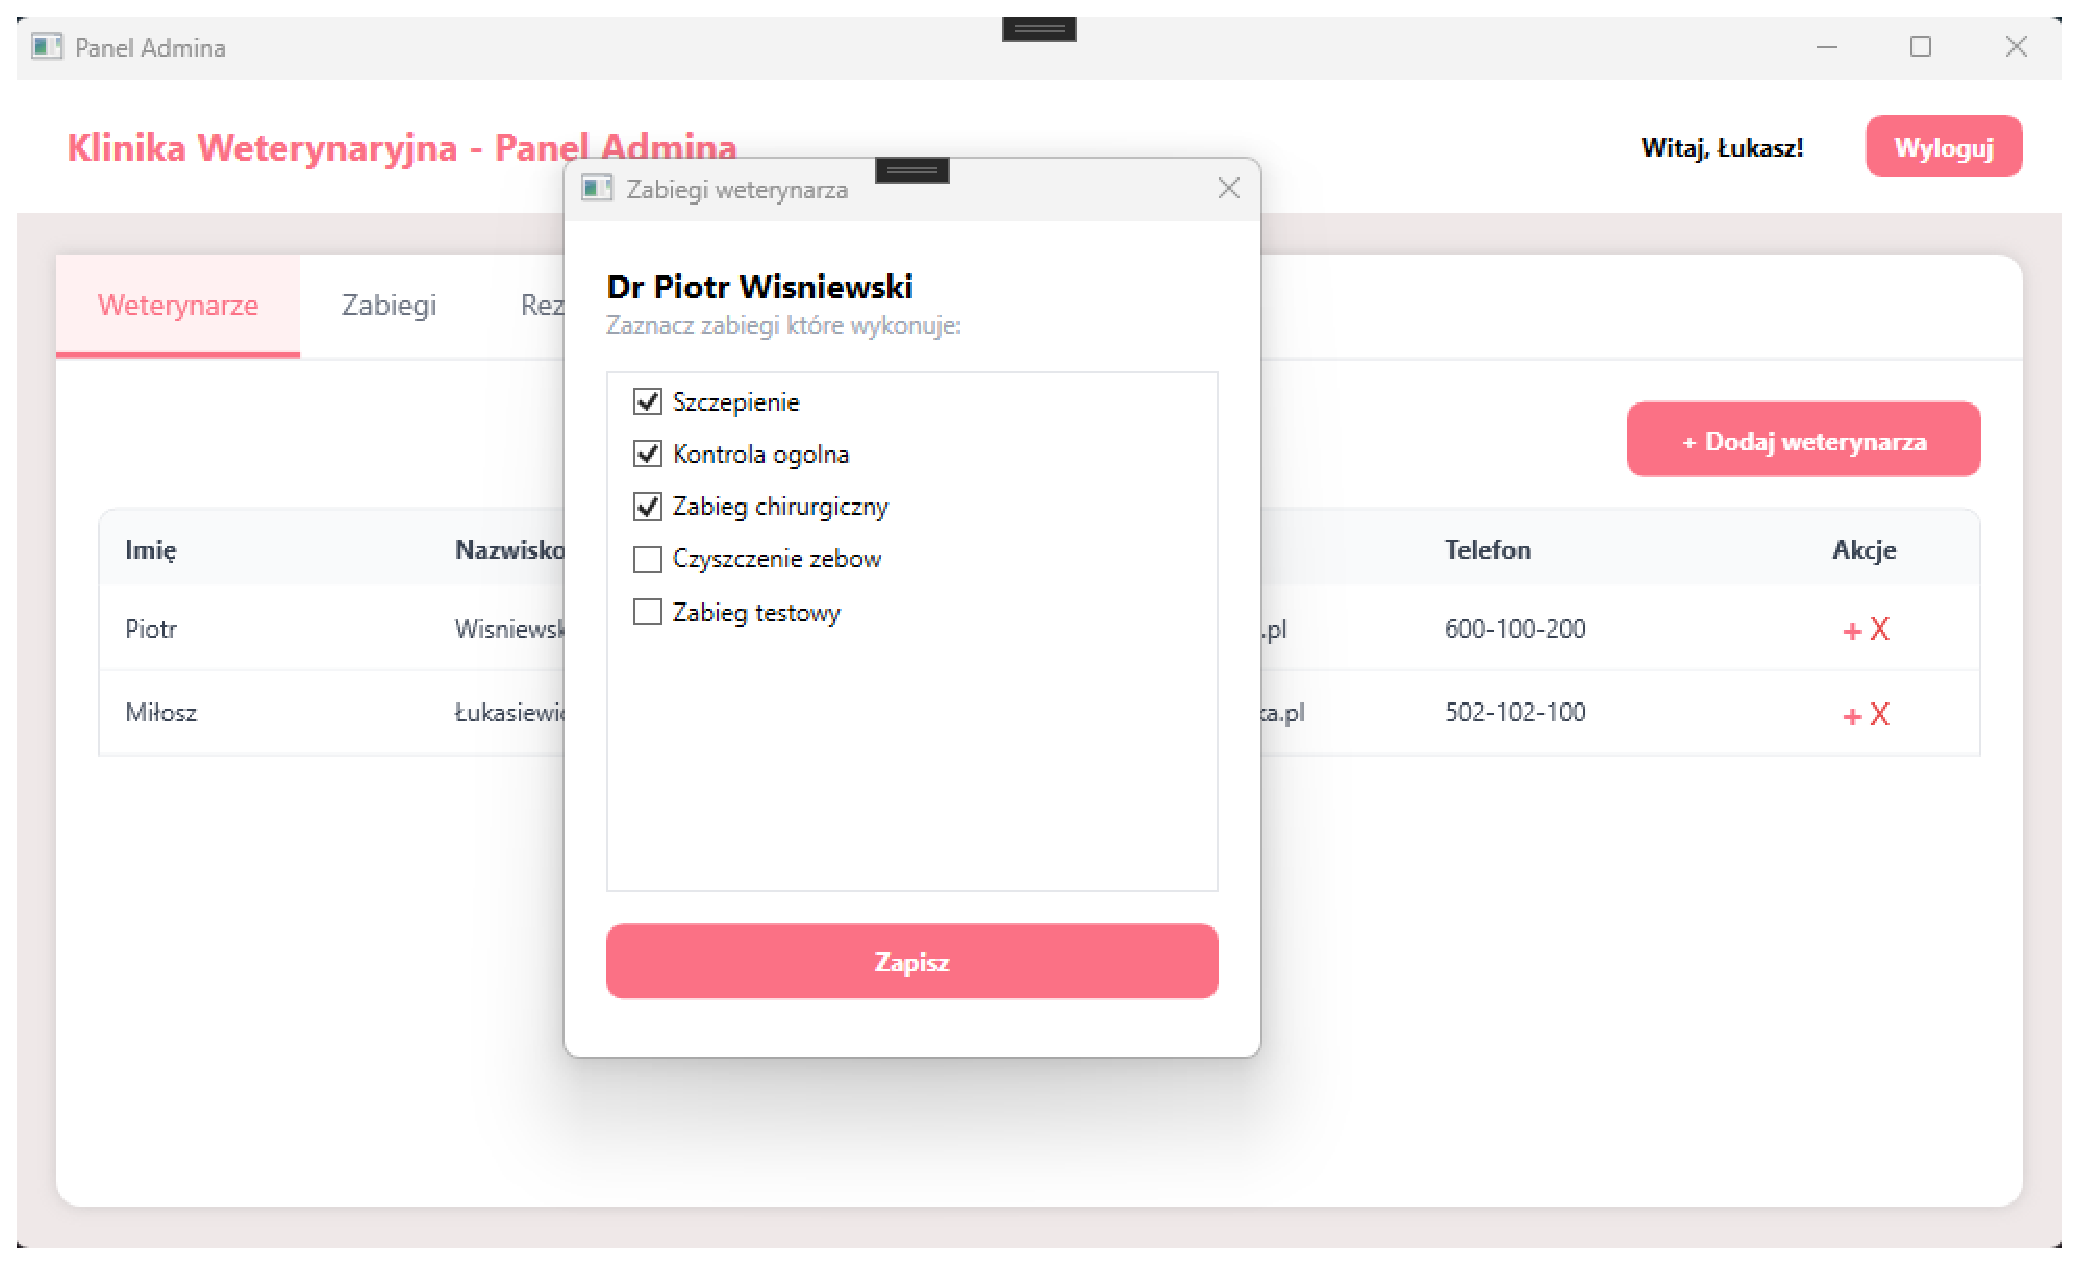
\includegraphics[width=0.9\linewidth]{figures/Admin/fig_043.eps}
\caption{Okno zarządzania zabiegami weterynarza.\label{fig43}}
\end{figure}

Po kliknięciu przycisku Zapisz aplikacja aktualizuje przypisanie zabiegów do weterynarza w bazie danych i 
wyświetla komunikat potwierdzający pomyślne wykonanie operacji.

\begin{figure}[H]
\centering
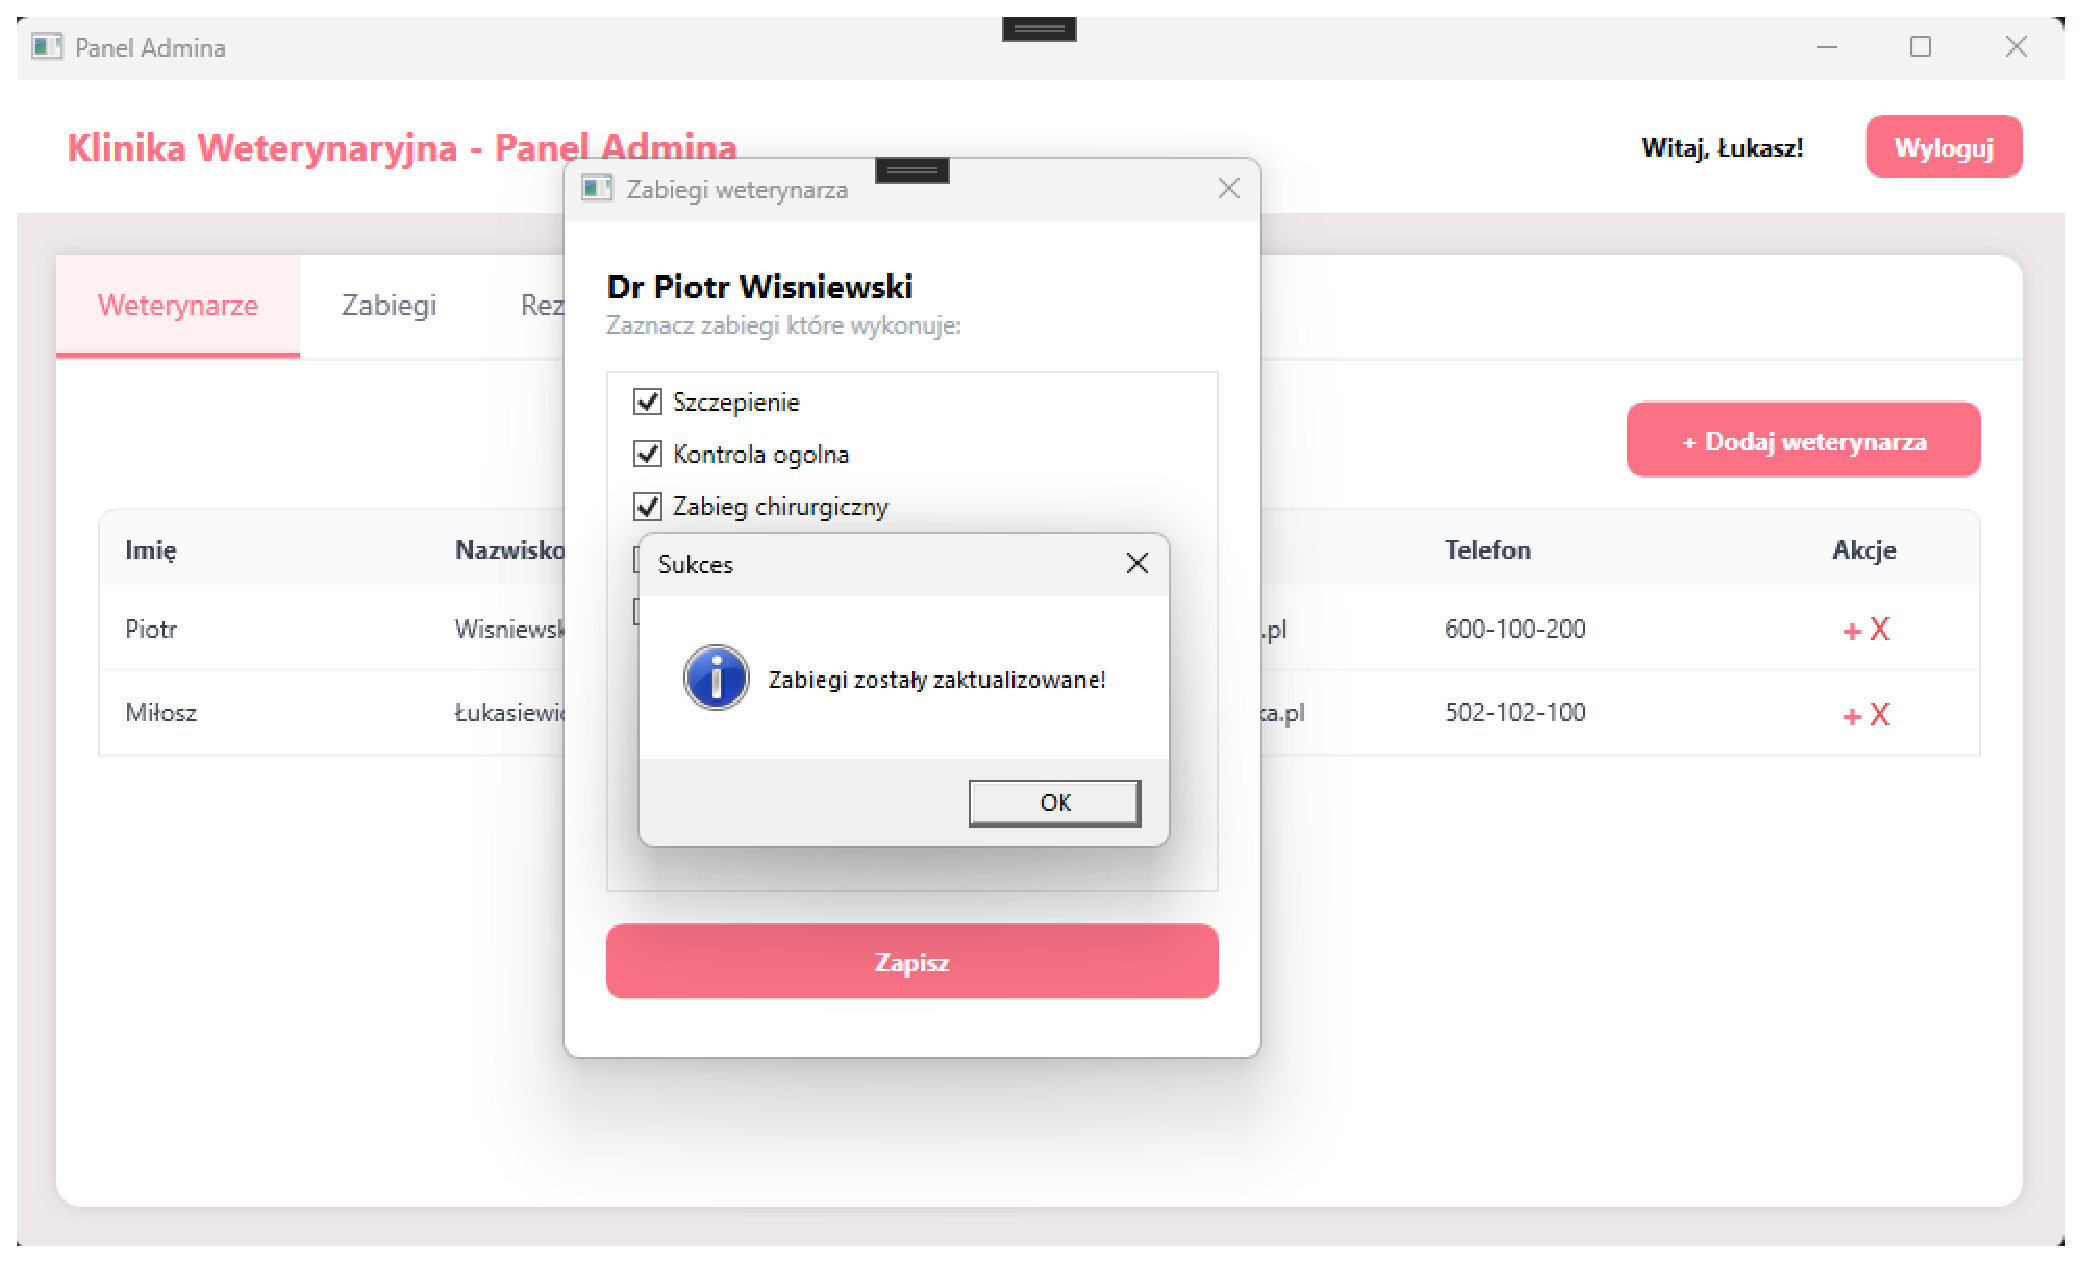
\includegraphics[width=0.9\linewidth]{figures/Admin/fig_044.eps}
\caption{Komunikat potwierdzający aktualizację zabiegów weterynarza.\label{fig44}}
\end{figure}

Po kliknięciu przycisku X przy wybranym weterynarzu aplikacja wyświetla okno dialogowe z prośbą o potwierdzenie operacji, 
informując że usunięcie weterynarza spowoduje również usunięcie jego dostępności i rezerwacji. 
Po potwierdzeniu weterynarz zostaje trwale usunięty z systemu.

\begin{figure}[H]
\centering
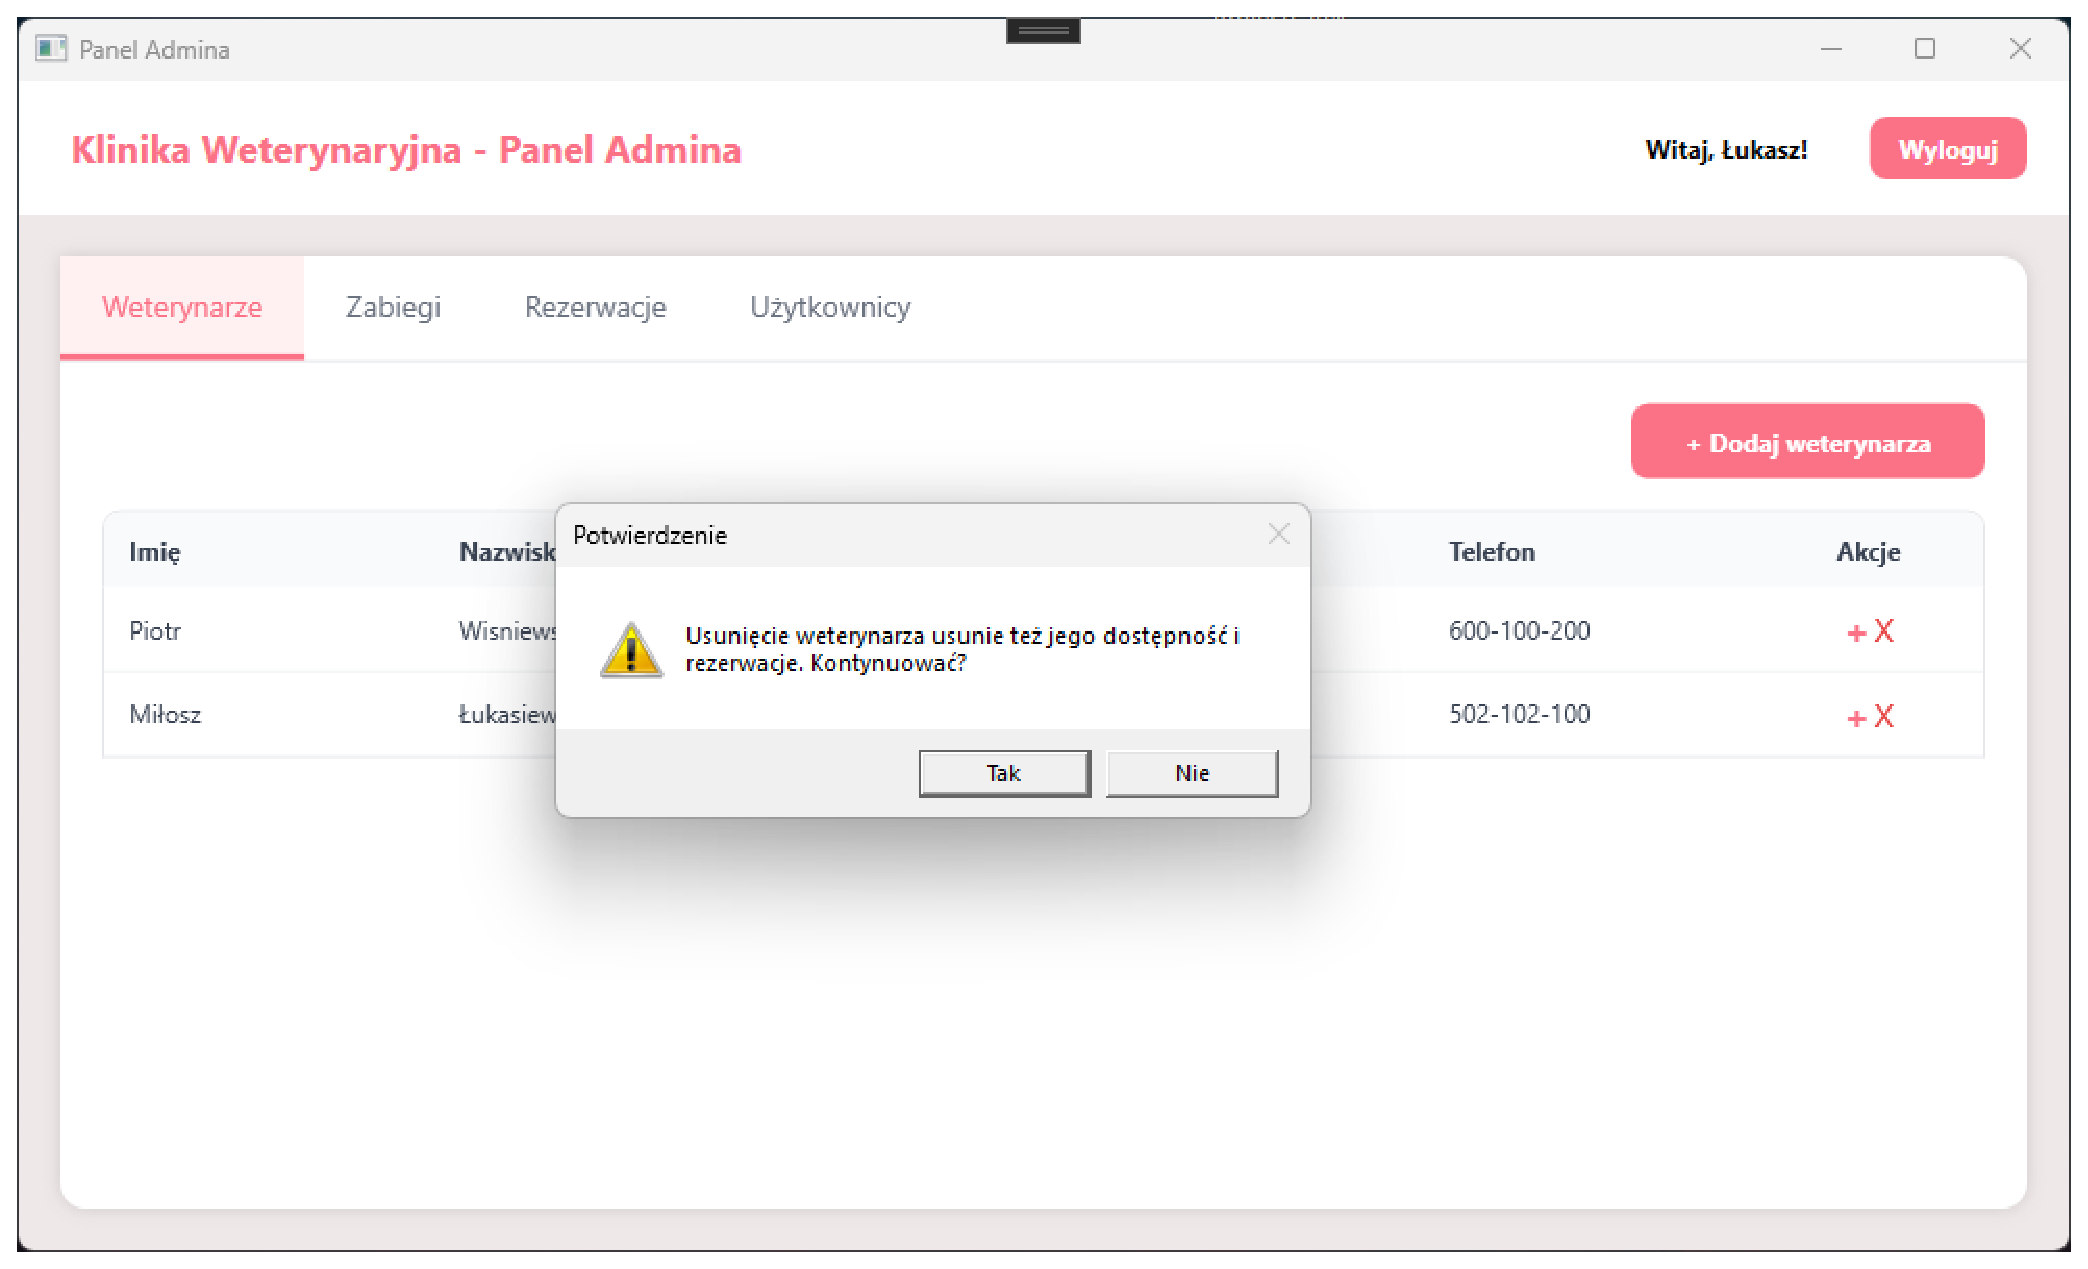
\includegraphics[width=0.9\linewidth]{figures/Admin/fig_045.eps}
\caption{Okno potwierdzenia usunięcia weterynarza.\label{fig45}}
\end{figure}

\textbf{Zakładka "Zabiegi"}

Zakładka "Zabiegi" wyświetla listę wszystkich zabiegów dostępnych w klinice. Dla każdego zabiegu prezentowane są 
informacje takie jak nazwa, czas trwania w minutach oraz cena. Przy każdym zabiegu dostępny jest przycisk X umożliwiający 
usunięcie zabiegu z systemu. W prawym górnym rogu zakładki znajduje się przycisk (+ Dodaj zabieg).

\begin{figure}[H]
\centering
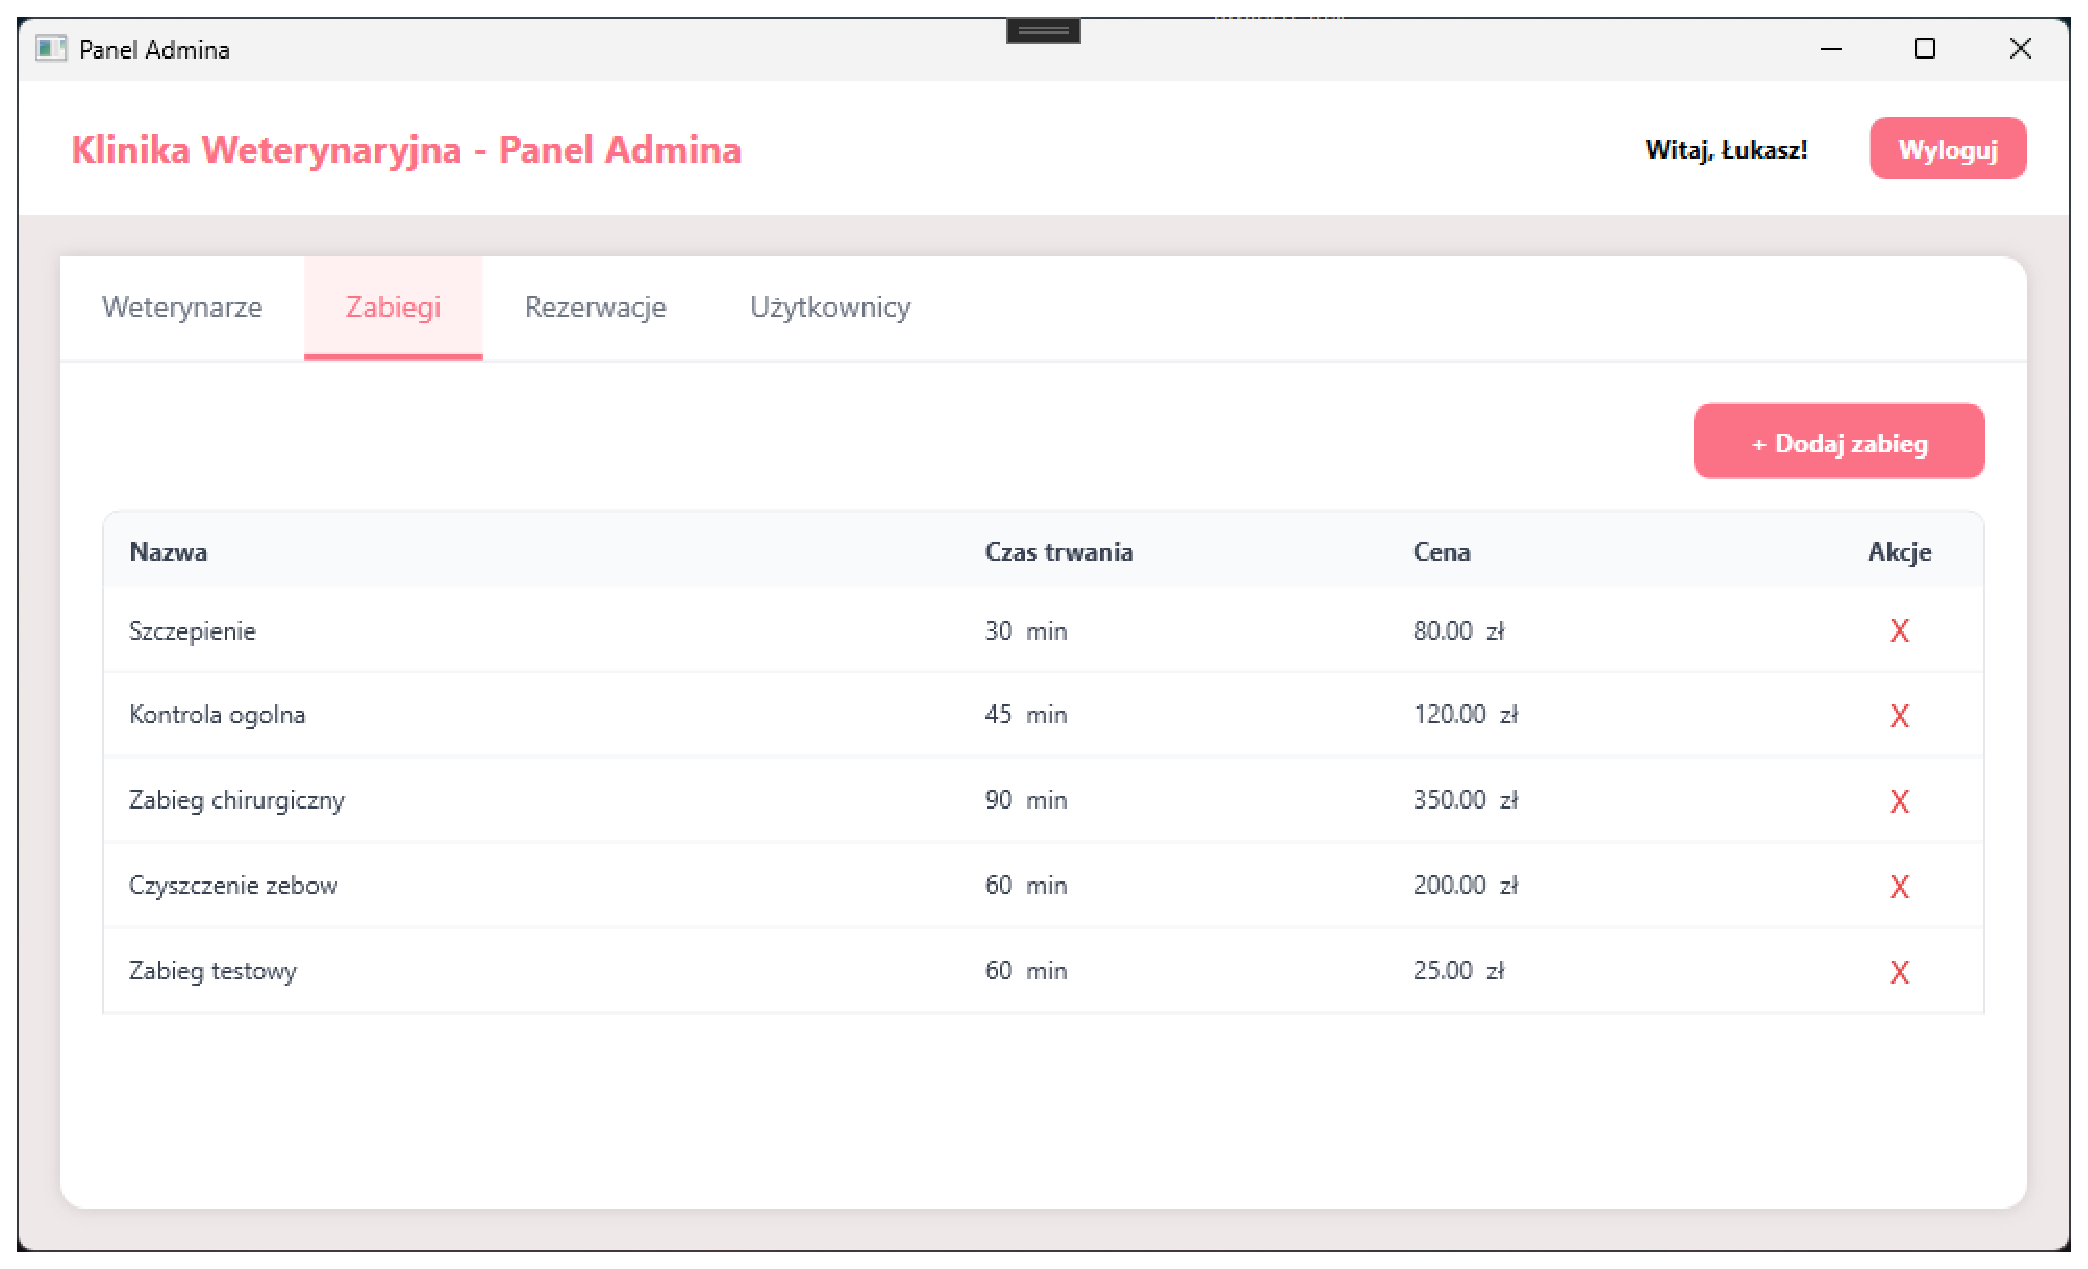
\includegraphics[width=0.9\linewidth]{figures/Admin/fig_046.eps}
\caption{Widok zakładki Zabiegi w panelu administratora.\label{fig46}}
\end{figure}

Po kliknięciu przycisku (+ Dodaj zabieg) otwierane jest okno formularza zawierające 
trzy pola: nazwa zabiegu, czas trwania w minutach oraz cena w złotych.

\begin{figure}[H]
\centering
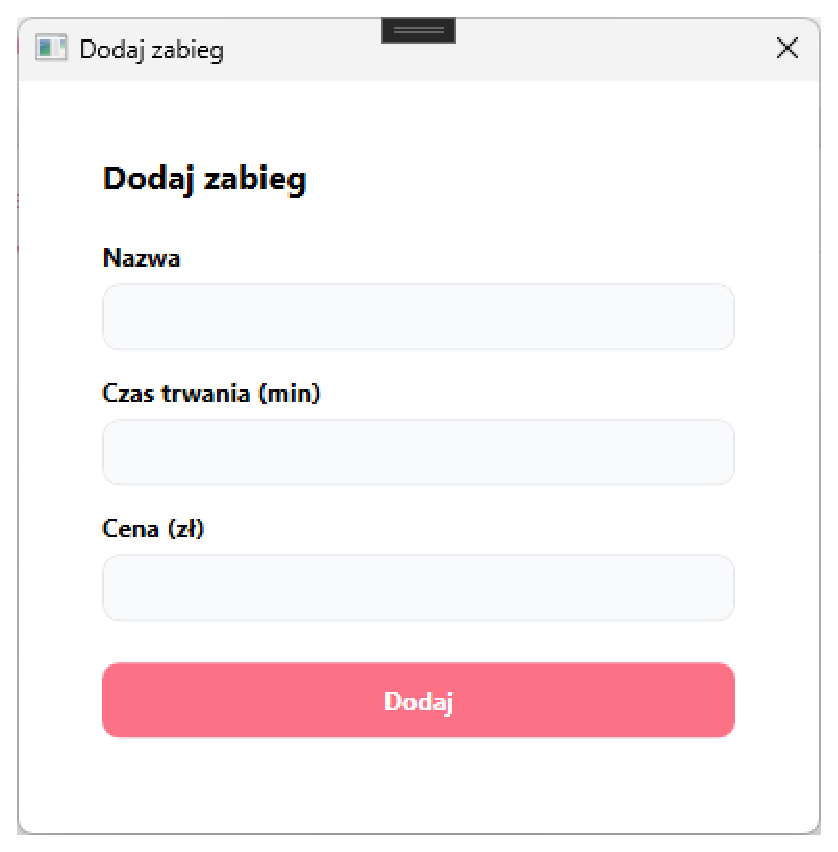
\includegraphics[width=0.55\linewidth]{figures/Admin/fig_047.eps}
\caption{Okno formularza dodawania zabiegu.\label{fig47}}
\end{figure}

W przypadku gdy administrator nie wypełni wszystkich pól formularza, aplikacja wyświetla komunikat błędu.

\begin{figure}[H]
\centering
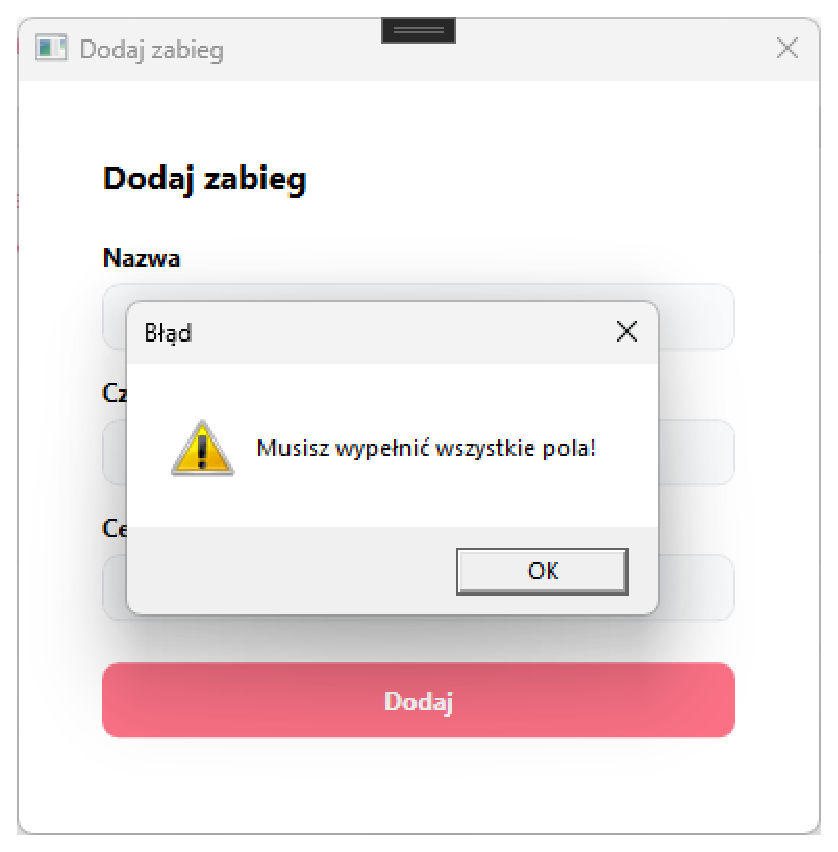
\includegraphics[width=0.55\linewidth]{figures/Admin/fig_048.eps}
\caption{Komunikat błędu przy niewypełnionych polach formularza.\label{fig48}}
\end{figure}

Aplikacja waliduje również poprawność podanego czasu trwania tzn. musi być dodatnią liczbą całkowitą. 
W przypadku podania nieprawidłowej wartości wyświetlany jest komunikat błędu.

\begin{figure}[H]
\centering
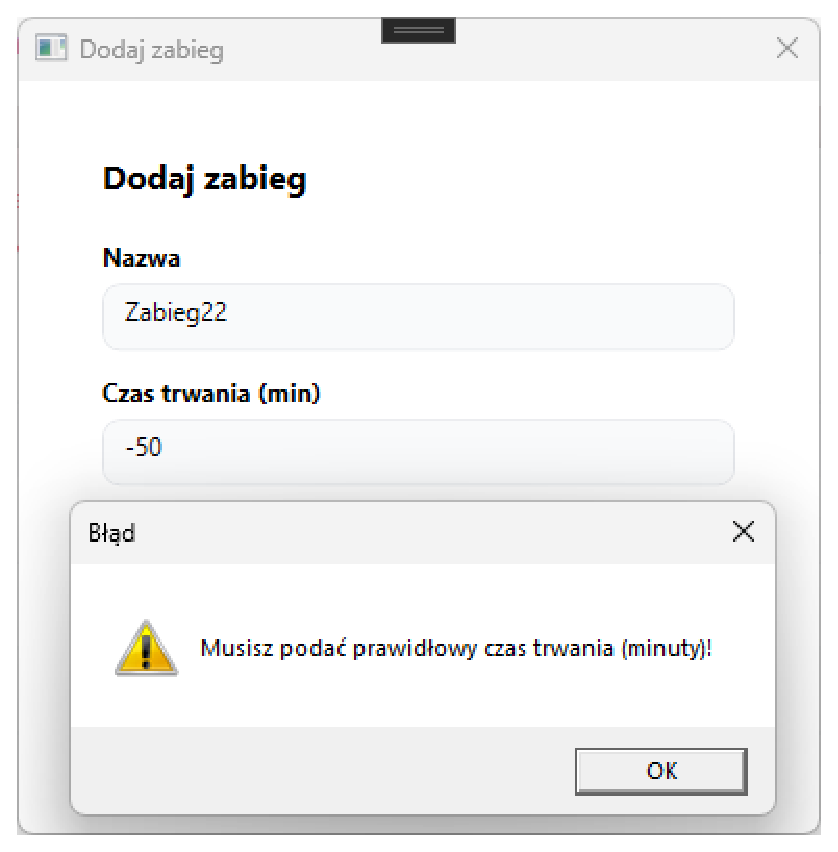
\includegraphics[width=0.55\linewidth]{figures/Admin/fig_049.eps}
\caption{Komunikat błędu przy nieprawidłowym czasie trwania zabiegu.\label{fig49}}
\end{figure}

Analogicznie walidowana jest cena zabiegu tzn. nie może być ona liczbą ujemną. W przypadku podania nieprawidłowej 
wartości wyświetlany jest odpowiedni komunikat błędu.

\begin{figure}[H]
\centering
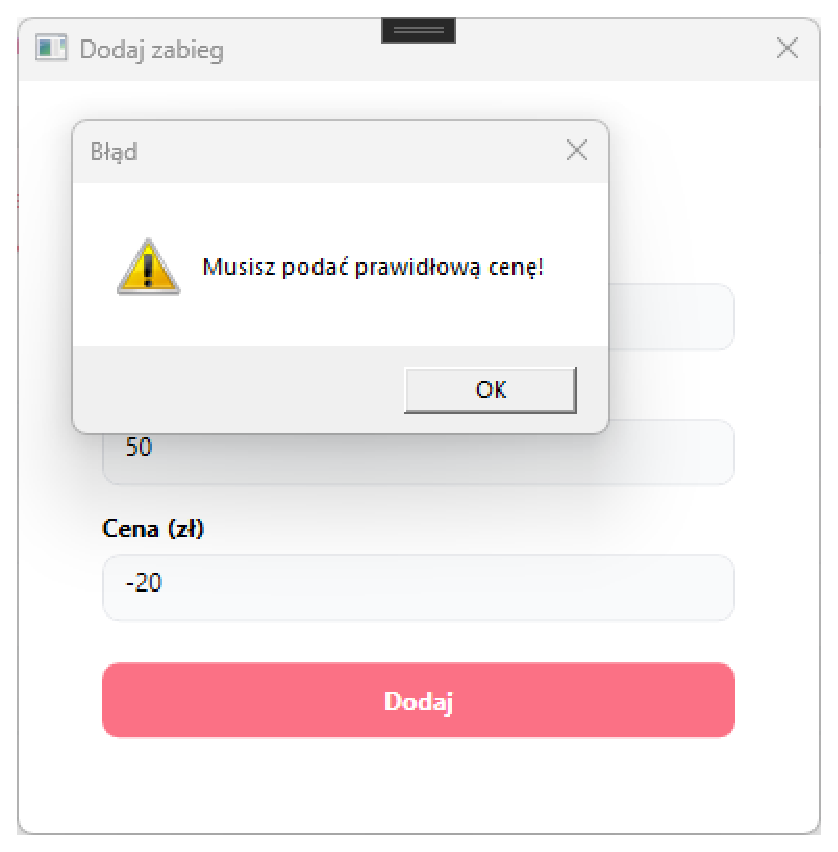
\includegraphics[width=0.55\linewidth]{figures/Admin/fig_050.eps}
\caption{Komunikat błędu przy nieprawidłowej cenie zabiegu.\label{fig50}}
\end{figure}

Po poprawnym wypełnieniu wszystkich pól i kliknięciu przycisku Dodaj nowy zabieg zostaje zapisany w bazie danych, a aplikacja 
wyświetla komunikat potwierdzający pomyślne dodanie zabiegu.

\begin{figure}[H]
\centering
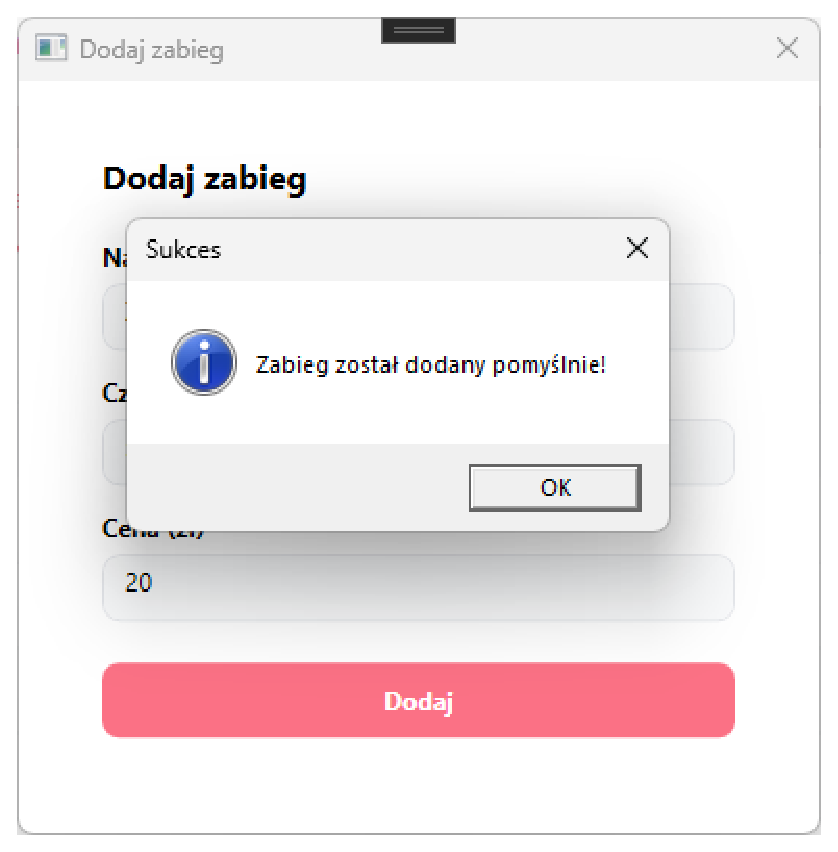
\includegraphics[width=0.55\linewidth]{figures/Admin/fig_051.eps}
\caption{Komunikat potwierdzający pomyślne dodanie zabiegu.\label{fig51}}
\end{figure}

Po kliknięciu przycisku X przy wybranym zabiegu aplikacja wyświetla okno dialogowe z prośbą o potwierdzenie operacji, informując 
że usunięcie zabiegu spowoduje również usunięcie powiązanych rezerwacji. Po potwierdzeniu zabieg zostaje trwale usunięty z systemu.

\begin{figure}[H]
\centering
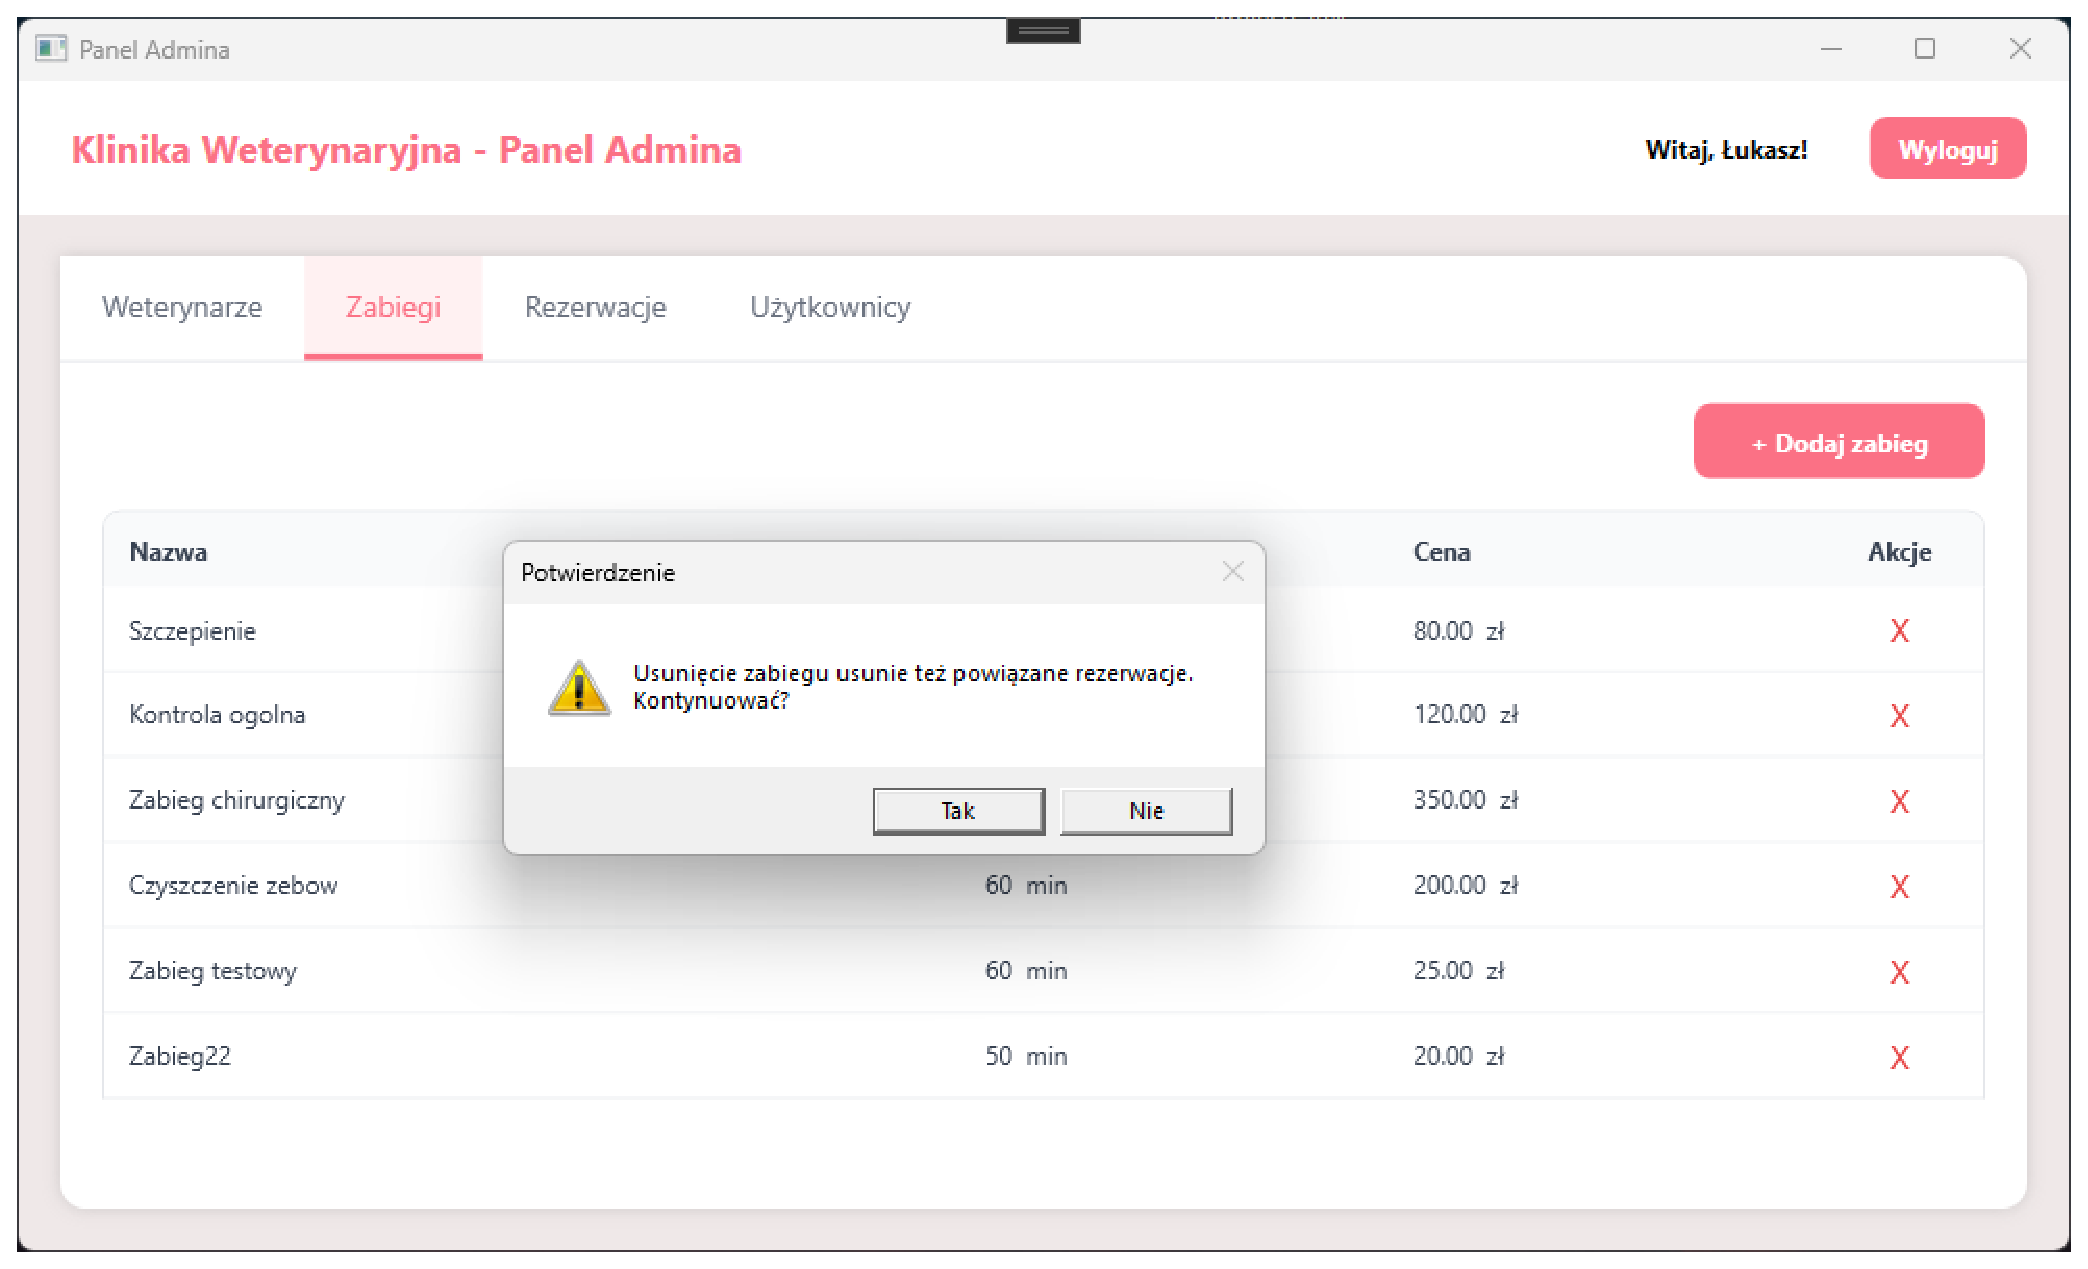
\includegraphics[width=0.9\linewidth]{figures/Admin/fig_052.eps}
\caption{Okno potwierdzenia usunięcia zabiegu.\label{fig52}}
\end{figure}

\textbf{Zakładka "Rezerwacje"}

Zakładka "Rezerwacje" wyświetla listę wszystkich rezerwacji wizyt w systemie. Dla każdej rezerwacji 
prezentowane są informacje takie jak data, godzina, imię i nazwisko weterynarza, imię pupila, nazwa zabiegu, imię i nazwisko 
właściciela oraz aktualny status wizyty. Administrator może zmieniać status każdej rezerwacji bezpośrednio z poziomu listy przy użyciu 
listy rozwijanej z trzema opcjami: Zarezerwowany, Zrealizowany oraz Anulowany. Nad listą dostępne są 
filtry: filtr daty, filtr weterynarza oraz filtr statusu, a także przycisk Wyczyść filtry resetujący wszystkie filtry do wartości domyślnych.

\begin{figure}[H]
\centering
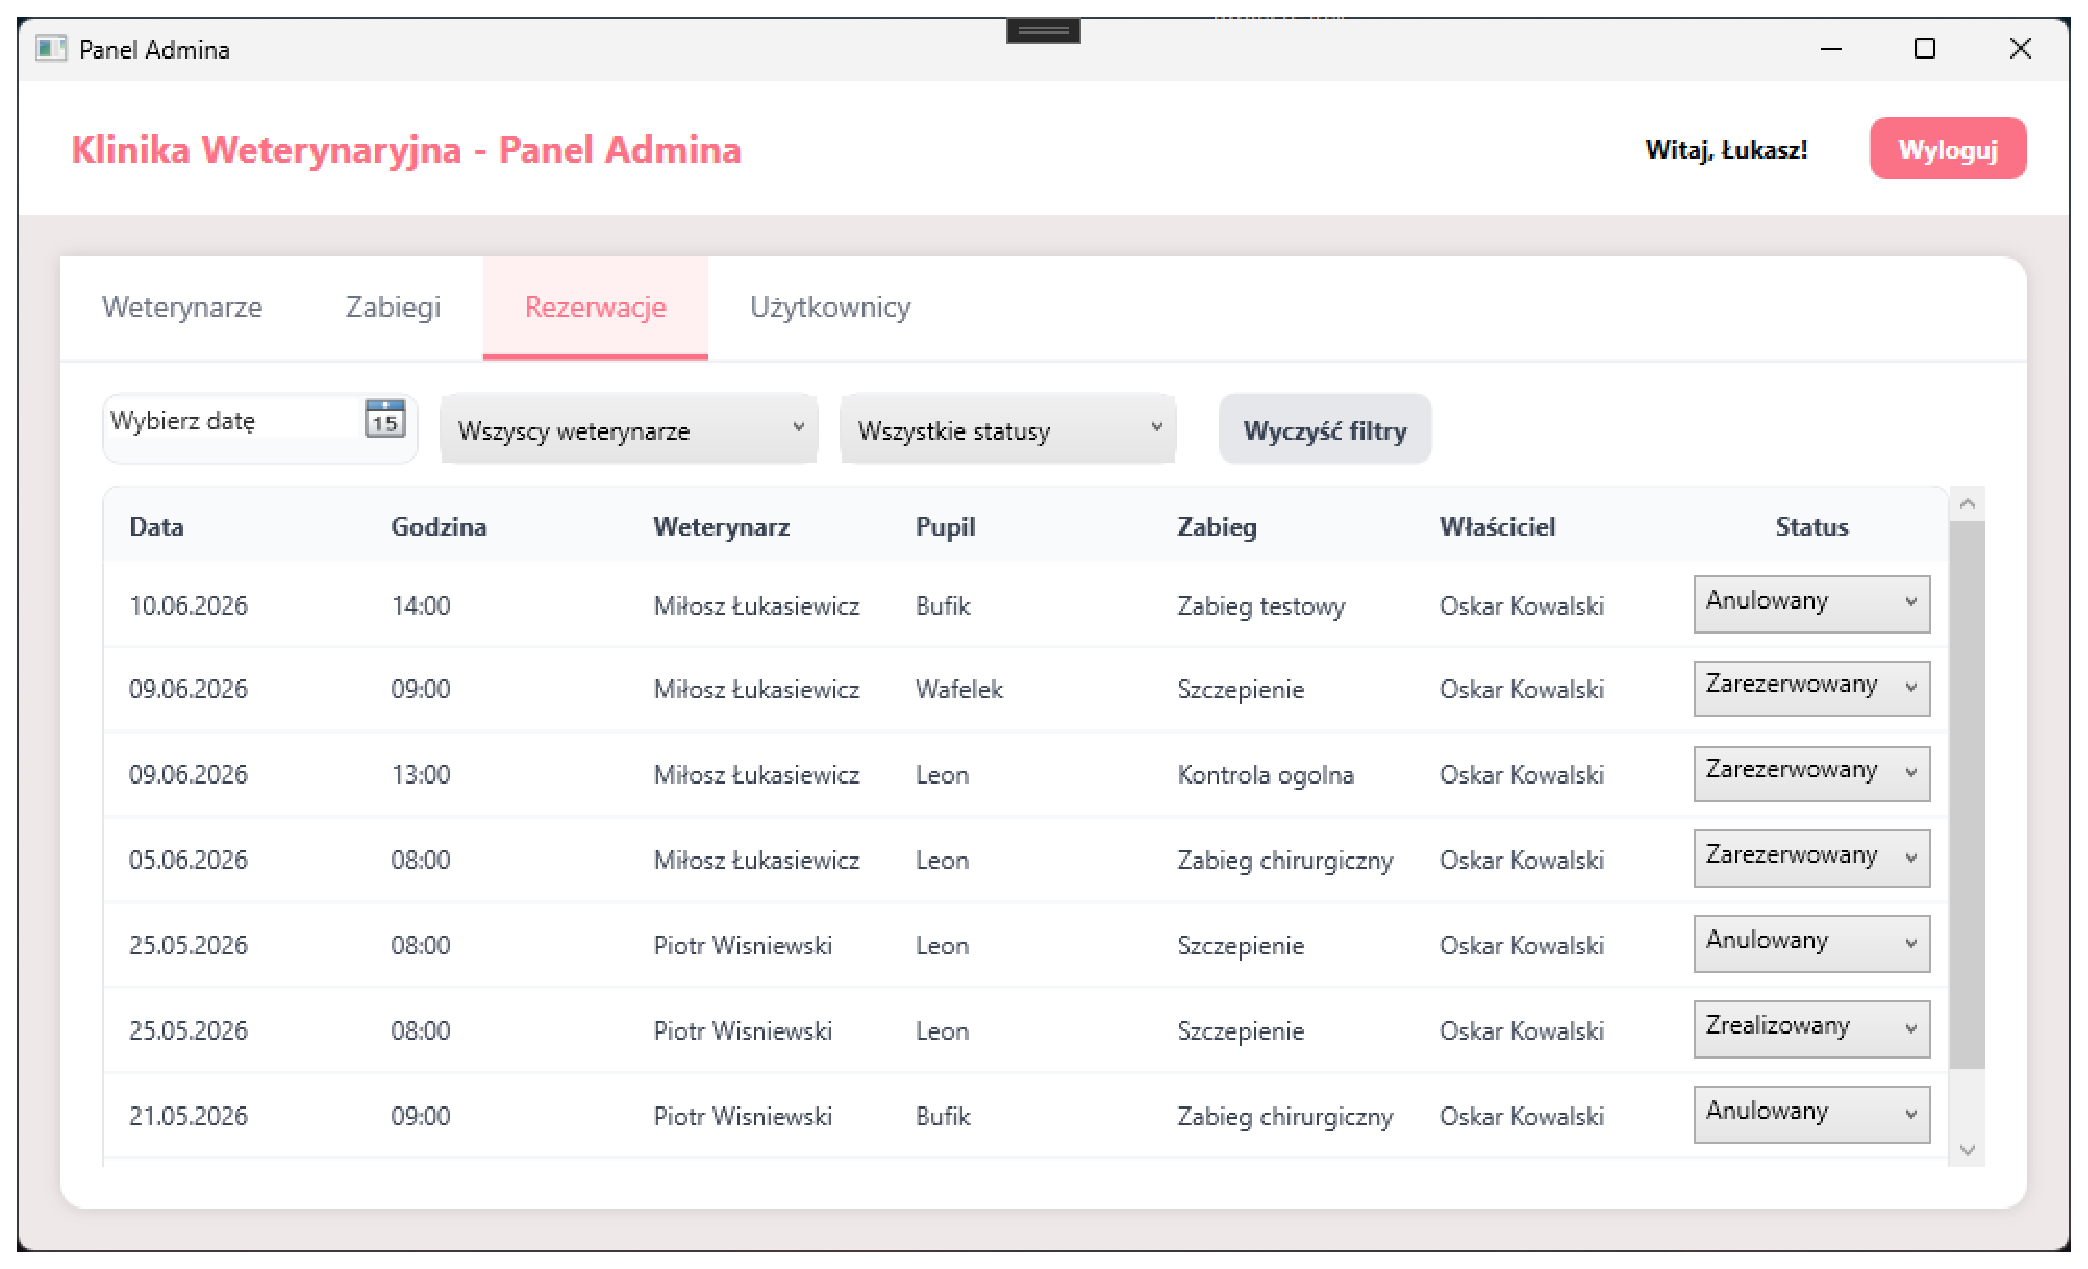
\includegraphics[width=0.9\linewidth]{figures/Admin/fig_053.eps}
\caption{Widok zakładki Rezerwacje w panelu administratora.\label{fig53}}
\end{figure}

Filtr daty umożliwia wyświetlenie wyłącznie rezerwacji z wybranego dnia. Poniżej przedstawiono widok po zastosowaniu 
filtra daty na dzień 25.05.2026 czyli lista zawiera tylko rezerwacje z tego dnia.

\begin{figure}[H]
\centering
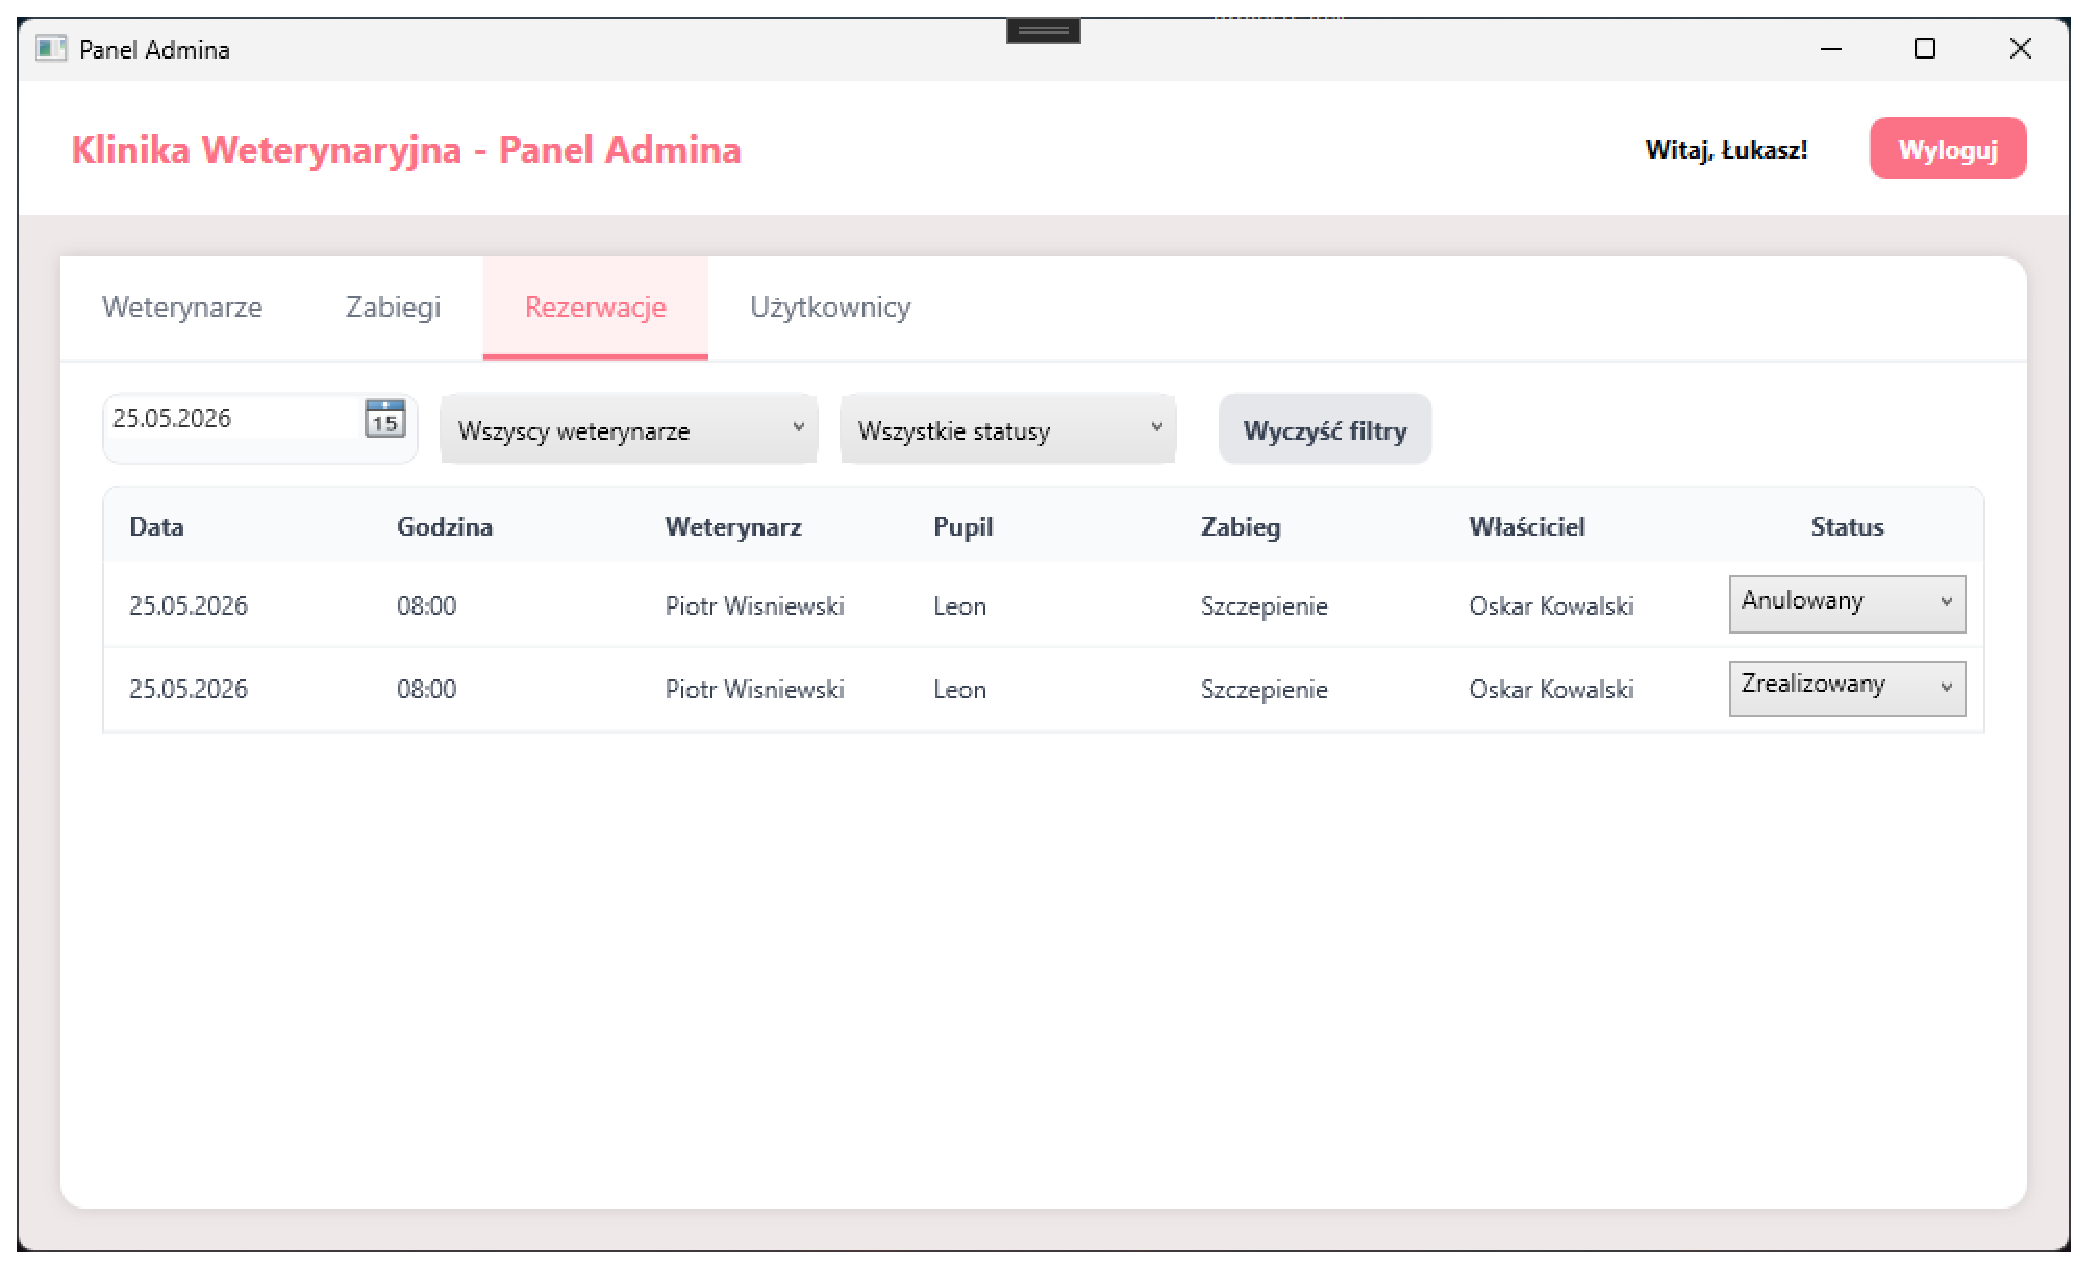
\includegraphics[width=0.9\linewidth]{figures/Admin/fig_054.eps}
\caption{Widok zakładki Rezerwacje po filtrowaniu po dacie.\label{fig54}}
\end{figure}

Filtr weterynarza umożliwia wyświetlenie wyłącznie rezerwacji przypisanych do wybranego weterynarza. 
Poniżej przedstawiono widok po wybraniu weterynarza Miłosz Łukasiewicz czyli lista zawiera tylko jego rezerwacje.

\begin{figure}[H]
\centering
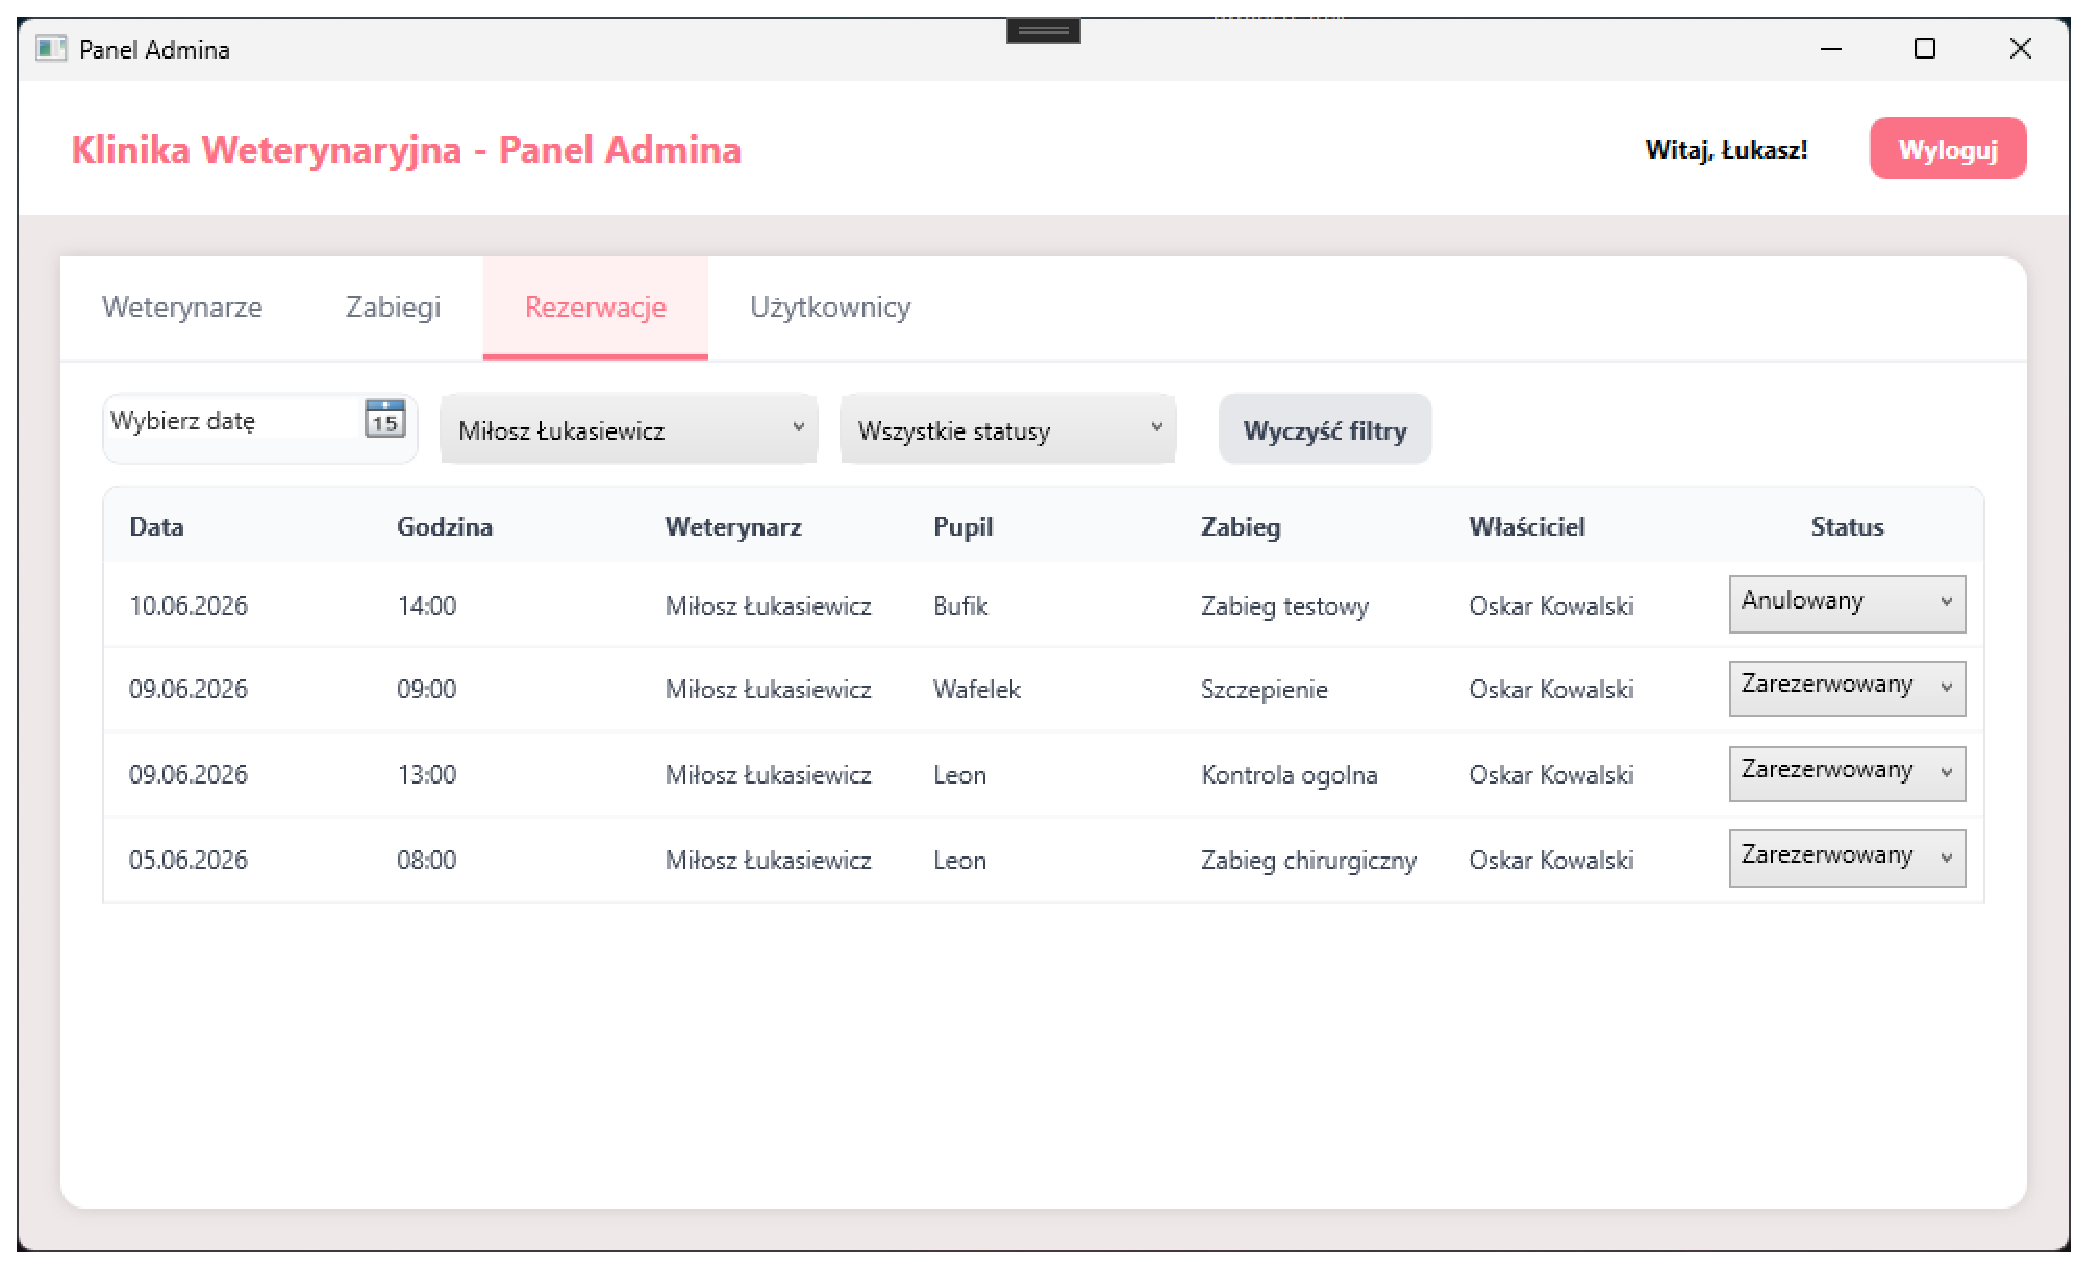
\includegraphics[width=0.9\linewidth]{figures/Admin/fig_055.eps}
\caption{Widok zakładki Rezerwacje po filtrowaniu po weterynarzu.\label{fig55}}
\end{figure}

Filtry można łączyć, poniżej przedstawiono widok po jednoczesnym zastosowaniu 
filtra weterynarza (Miłosz Łukasiewicz) oraz filtra statusu (Anulowany), co pozwala 
precyzyjnie odnaleźć konkretne rezerwacje spełniające oba kryteria.

\begin{figure}[H]
\centering
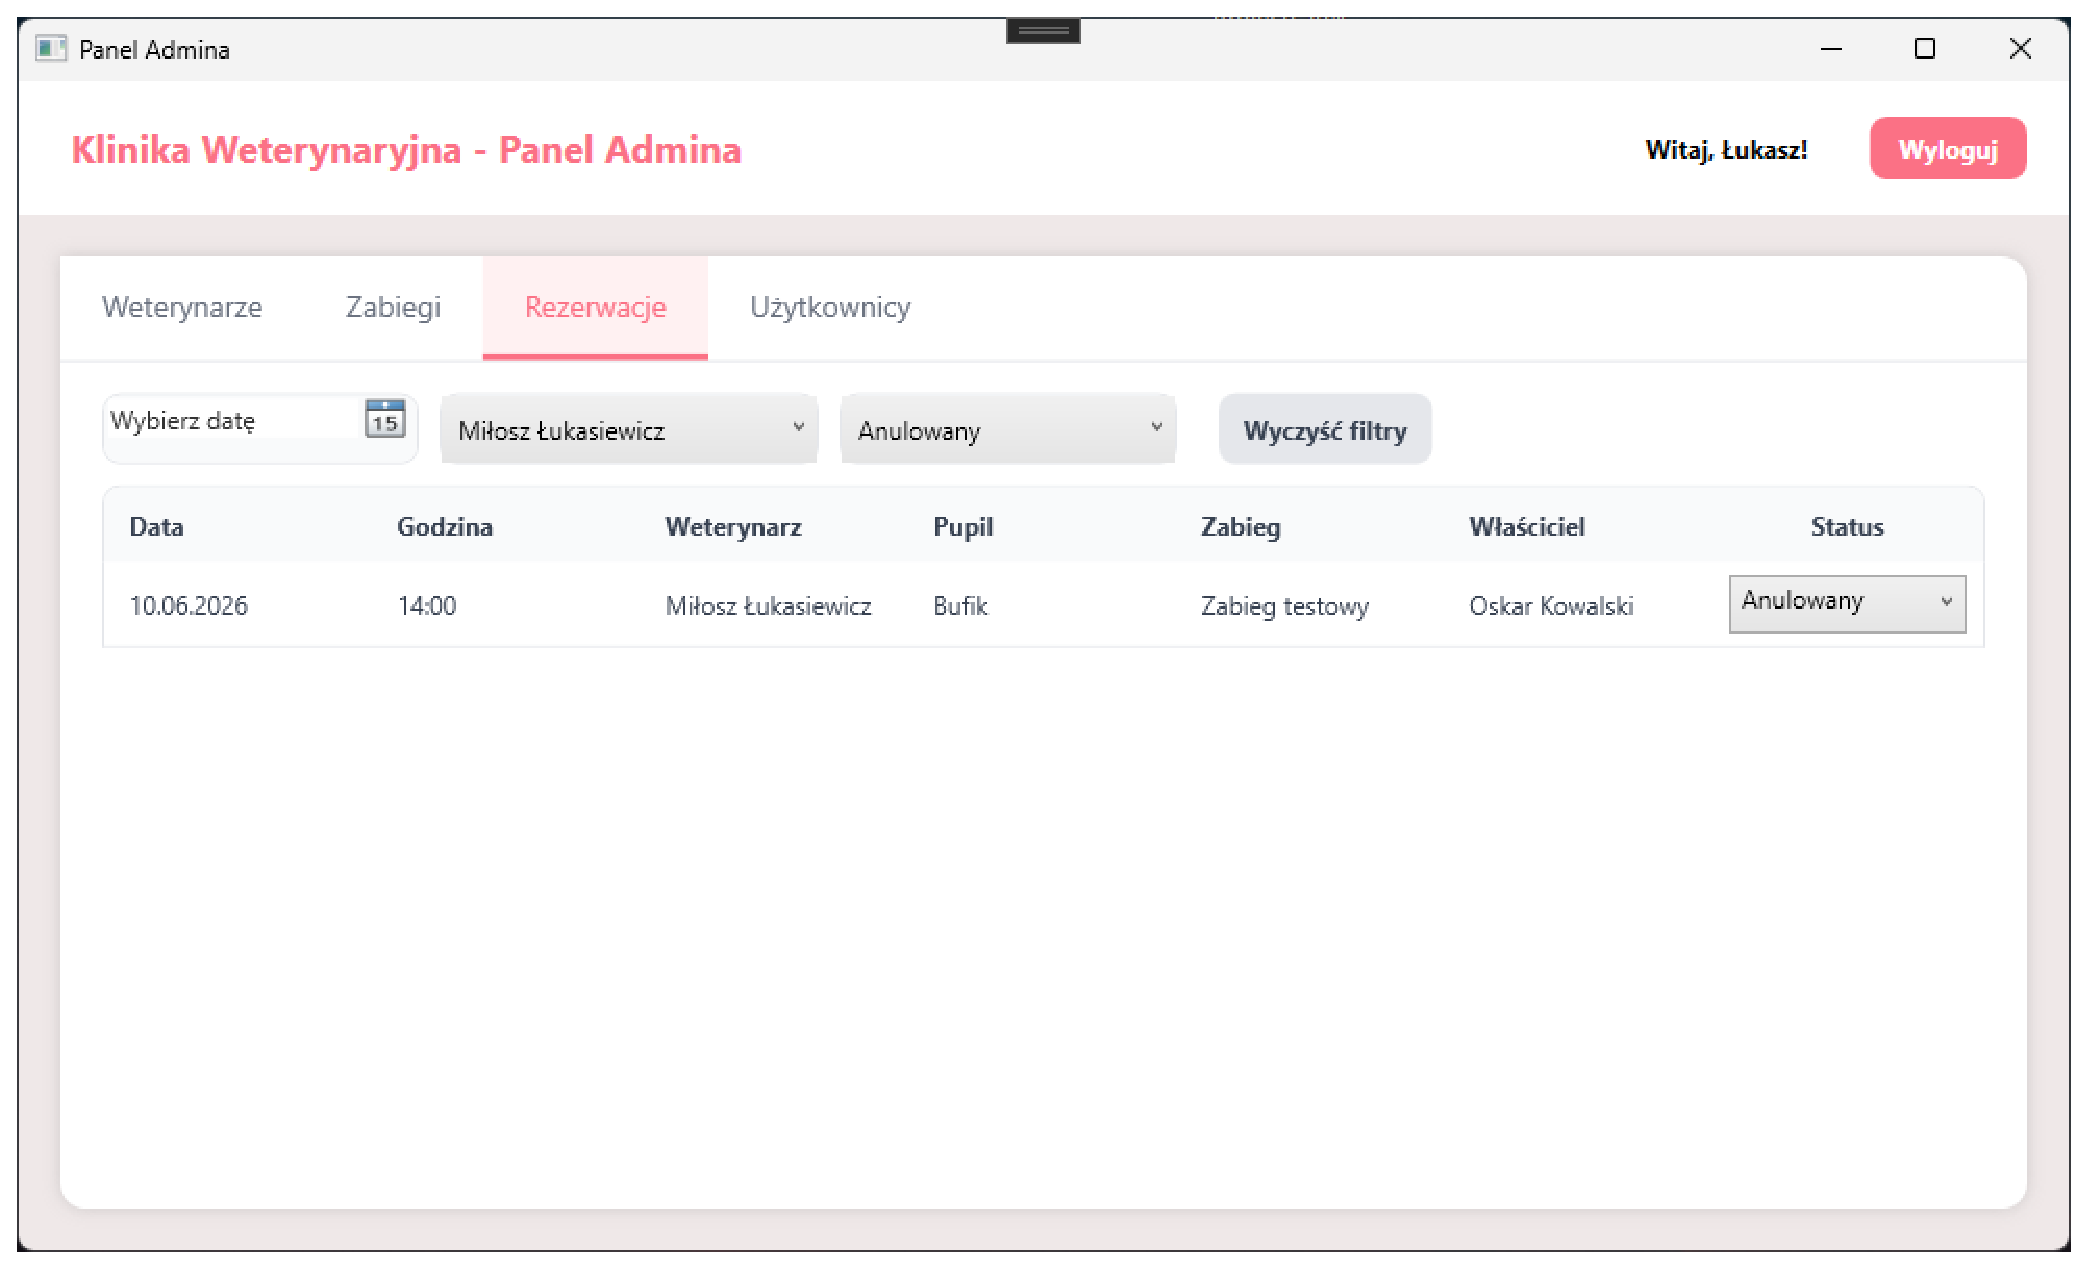
\includegraphics[width=0.9\linewidth]{figures/Admin/fig_056.eps}
\caption{Widok zakładki Rezerwacje po filtrowaniu po weterynarzu i statusie.\label{fig56}}
\end{figure}

\textbf{Zakładka "Użytkownicy"}

Zakładka "Użytkownicy" wyświetla listę wszystkich zarejestrowanych użytkowników systemu z rolą Uzytkownik. Dla każdego 
użytkownika prezentowane są informacje takie jak imię, nazwisko, adres e-mail, numer telefonu oraz aktualne saldo konta. 
Przy każdym użytkowniku dostępny jest przycisk X umożliwiający usunięcie użytkownika z systemu.

\begin{figure}[H]
\centering
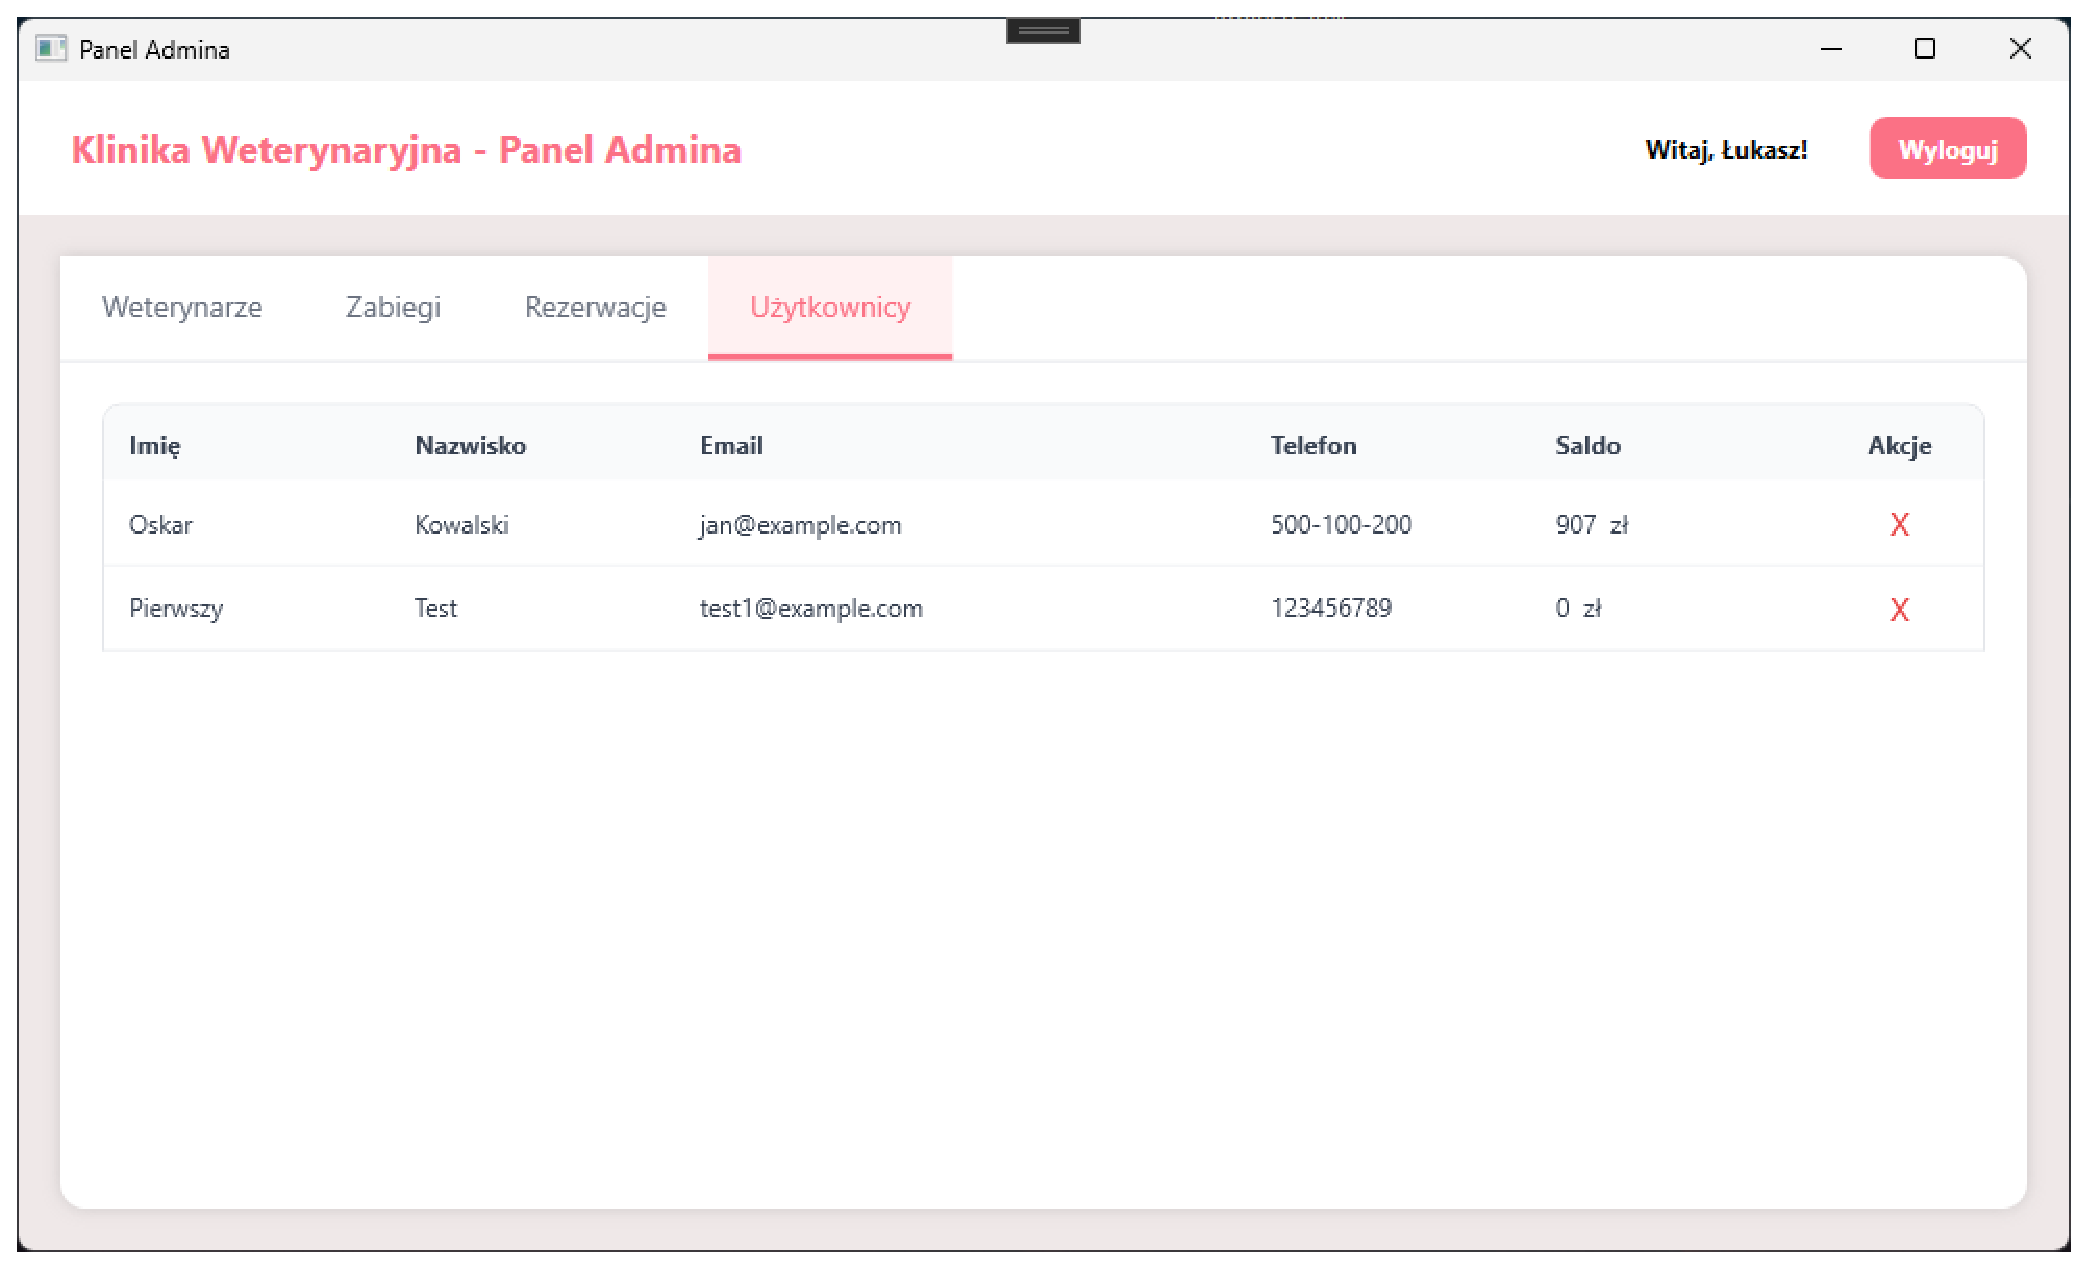
\includegraphics[width=0.9\linewidth]{figures/Admin/fig_057.eps}
\caption{Widok zakładki Użytkownicy w panelu administratora.\label{fig57}}
\end{figure}

Po kliknięciu przycisku X przy wybranym użytkowniku aplikacja wyświetla okno dialogowe z prośbą o 
potwierdzenie operacji, informując że usunięcie użytkownika spowoduje również usunięcie 
jego pupili i rezerwacji. Po potwierdzeniu użytkownik zostaje trwale usunięty z systemu 
wraz ze wszystkimi powiązanymi danymi, a lista użytkowników jest automatycznie odświeżana.

\begin{figure}[H]
\centering
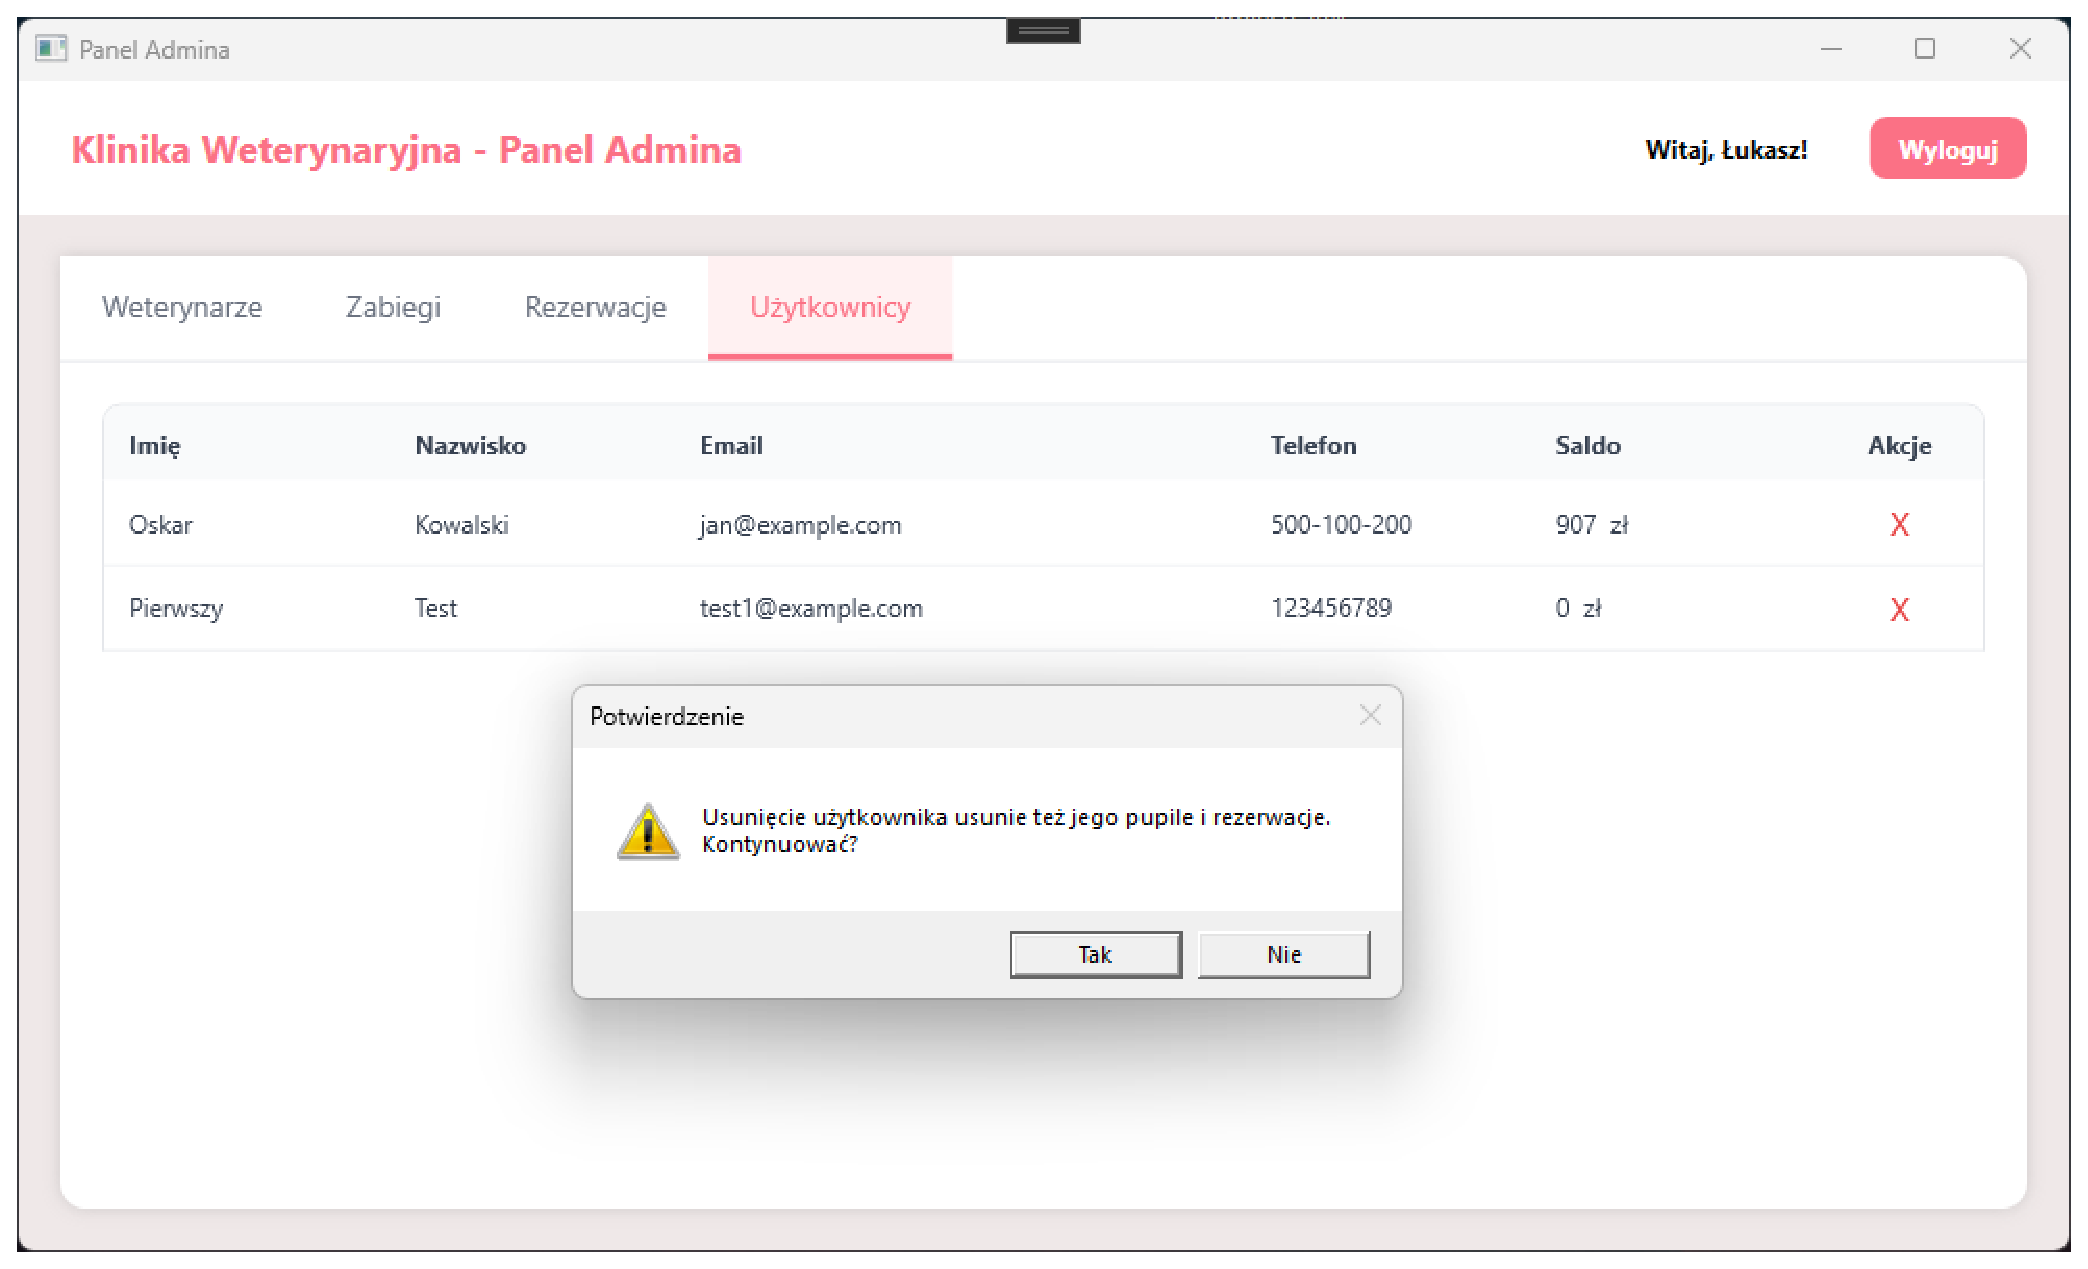
\includegraphics[width=0.9\linewidth]{figures/Admin/fig_058.eps}
\caption{Okno potwierdzenia usunięcia użytkownika.\label{fig58}}
\end{figure}

\section{Uruchomienie aplikacji}

\begin{enumerate}
\item Sklonować/Pobrać repozytorium projektu z GitHub: 
\url{https://github.com/lukaszwarzocha/Programowanie_Obiektowe2.git}
\item Otworzyć folder Projekt\_PO\_KW w Visual Studio Insiders.
\item Utworzyć bazę danych SQL Server o nazwie "klinika\_weterynaryjna" i zaimportować do niej strukturę 
oraz dane z pliku schema.sql znajdującego się w katalogu Dokumentacja.
\item Upewnić się że connection string w pliku Database.cs jest poprawny:
\begin{lstlisting}
Server=localhost;Database=klinika_weterynaryjna;
Trusted_Connection=True;TrustServerCertificate=True;
\end{lstlisting}
\item Przywrócić pakiety NuGet. W tym celu kliknąć prawym przyciskiem myszy na rozwiązanie w Eksploratorze rozwiązań, a następnie wybrać 
Menedżer pakietów NuGet $\rightarrow$ Przywróć pakiety NuGet.
\item Zbudować rozwiązanie: Kompilacja $\rightarrow$ Kompiluj rozwiązanie lub skrótem klawiszowum Ctrl+B.
\item Uruchomić aplikację klawiszem F5 lub przyciskiem Start.
\end{enumerate}

\textbf{Dane do logowania}

W celu zalogowania się na konto administratora należy wykorzystać następujące dane:
\begin{itemize}
\item Login: admin@example.com
\item Hasło: haslo123
\end{itemize}

W celu zalogowania się na konto użytkownika można wykorzystać następujące dane:
\begin{itemize}
\item Login: jan@example.com
\item Hasło: haslo1234
\end{itemize}





